%%%%%%%%%%%%%%%%%%%%%%%%%%%%%%%%%%%%%%%%%%%%%%%%%%%%%%%
\documentclass{article}
%%%%%%%%%%%%%%%%%%%%%%%%%%%%%%%%%%%%%%%%%%%%%%%%%%%%%%%
\usepackage[utf8]{vietnam}
%%%%%%%%%%%%%%%%%%%%%%%%%%%%%%%%%%%%%%%%%%%%%%%%%%%%%%%
\usepackage{graphicx}
%%%%%%%%%%%%%%%%%%%%%%%%%%%%%%%%%%%%%%%%%%%%%%%%%%%%%%%
\usepackage{hyperref}
%%%%%%%%%%%%%%%%%%%%%%%%%%%%%%%%%%%%%%%%%%%%%%%%%%%%%%%
\usepackage{xcolor}
\pagecolor[RGB]{40, 42, 54} % Đặt màu nền
\color[RGB]{18, 161, 24} % Đặt màu chữ
%%%%%%%%%%%%%%%%%%%%%%%%%%%%%%%%%%%%%%%%%%%%%%%%%%%%%%%
\usepackage{float} % Cố định hình ảnh [H]
%%%%%%%%%%%%%%%%%%%%%%%%%%%%%%%%%%%%%%%%%%%%%%%%%%%%%%%
\begin{document}
%%%%%%%%%%%%%%%%%%%%%%%%%%%%%%%%%%%%%%%%%%%%%%%%%%%%%%%
\tableofcontents
\newpage
%%%%%%%%%%%%%%%%%%%%%%%%%%%%%%%%%%%%%%%%%%%%%%%%%%%%%%%
\listoffigures
\newpage
%%%%%%%%%%%%%%%%%%%%%%%%%%%%%%%%%%%%%%%%%%%%%%%%%%%%%%%
\section{Tuần 1: Thực hành tiền xử lý dữ liệu (ETL) cơ bản trong Excel}
%%%%%%%%%%%%%%%%%%%%%%%%%%%%%%%%%%%%%%%%%%%%%%%%%%%%%%
\subsection{Video 1}
%%%%%%%%%%%%%%%%%%%%%%%%%%%%%%%%%%%%%%%%%%%%%%%%%%%%%%%
\begin{figure}[H]
\centering
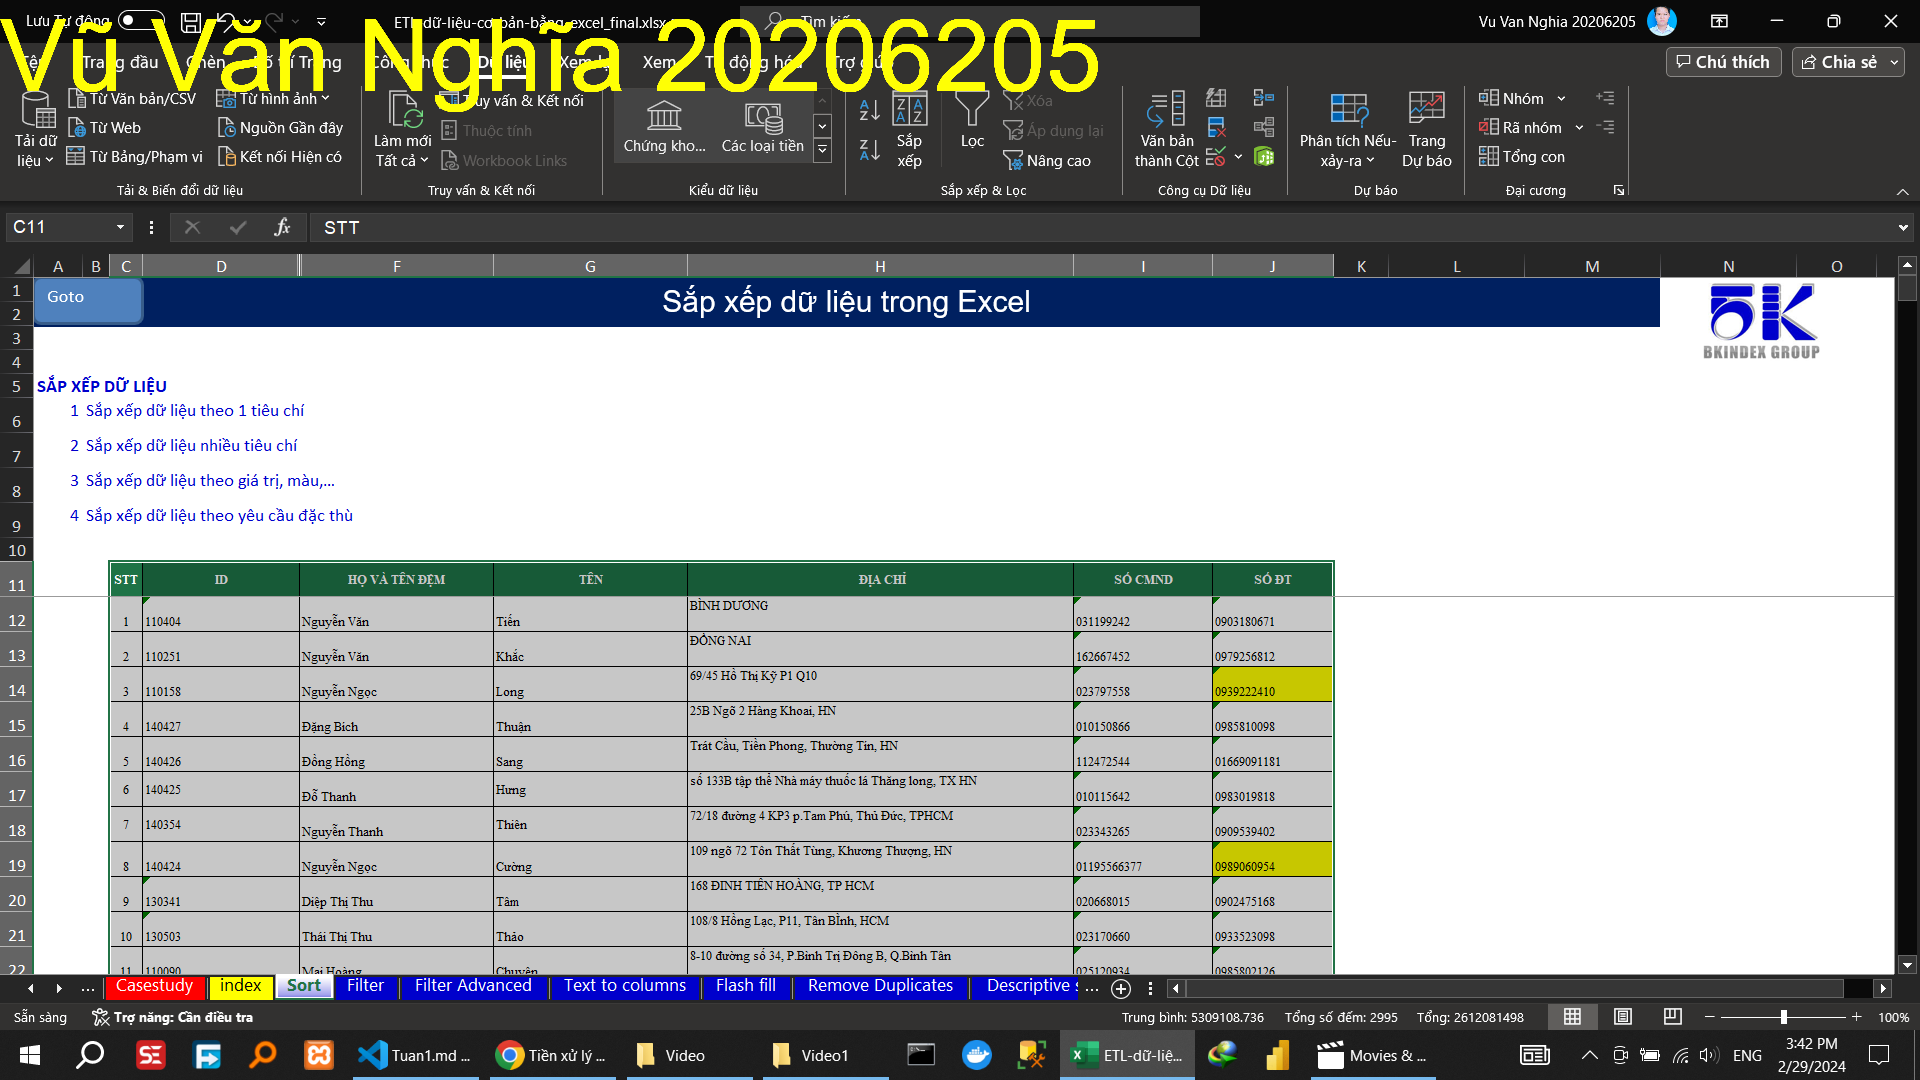
\includegraphics[scale = 0.15]{Video1/HuongDan/1.png}
\caption{Hướng dẫn sắp xếp dữ liệu theo 1 tiêu chí là số thứ tự}
\end{figure}

\begin{figure}[H]
\centering
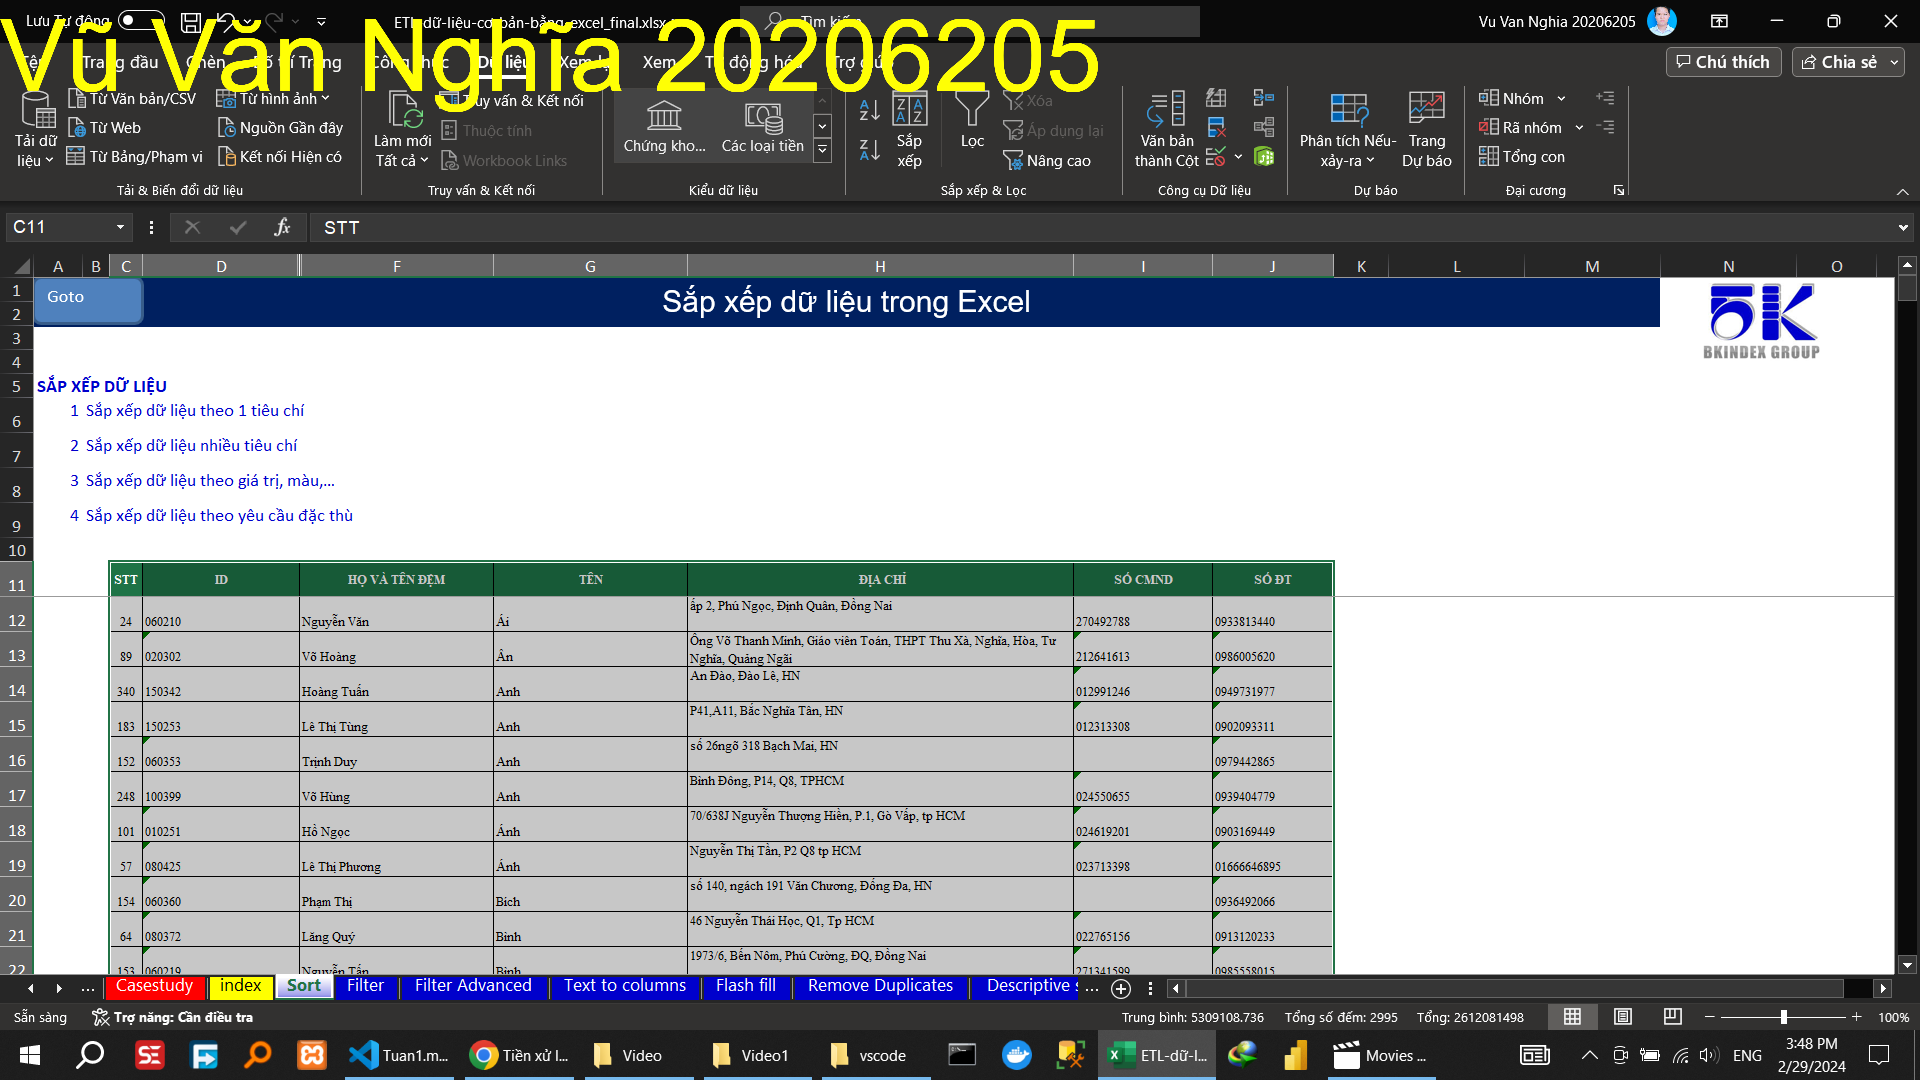
\includegraphics[scale = 0.15]{Video1/HuongDan/2.png}
\caption{Hướng dẫn sắp xếp dữ liệu theo nhiều tiêu chí họ và tên đệm}
\end{figure}

\begin{figure}[H]
\centering
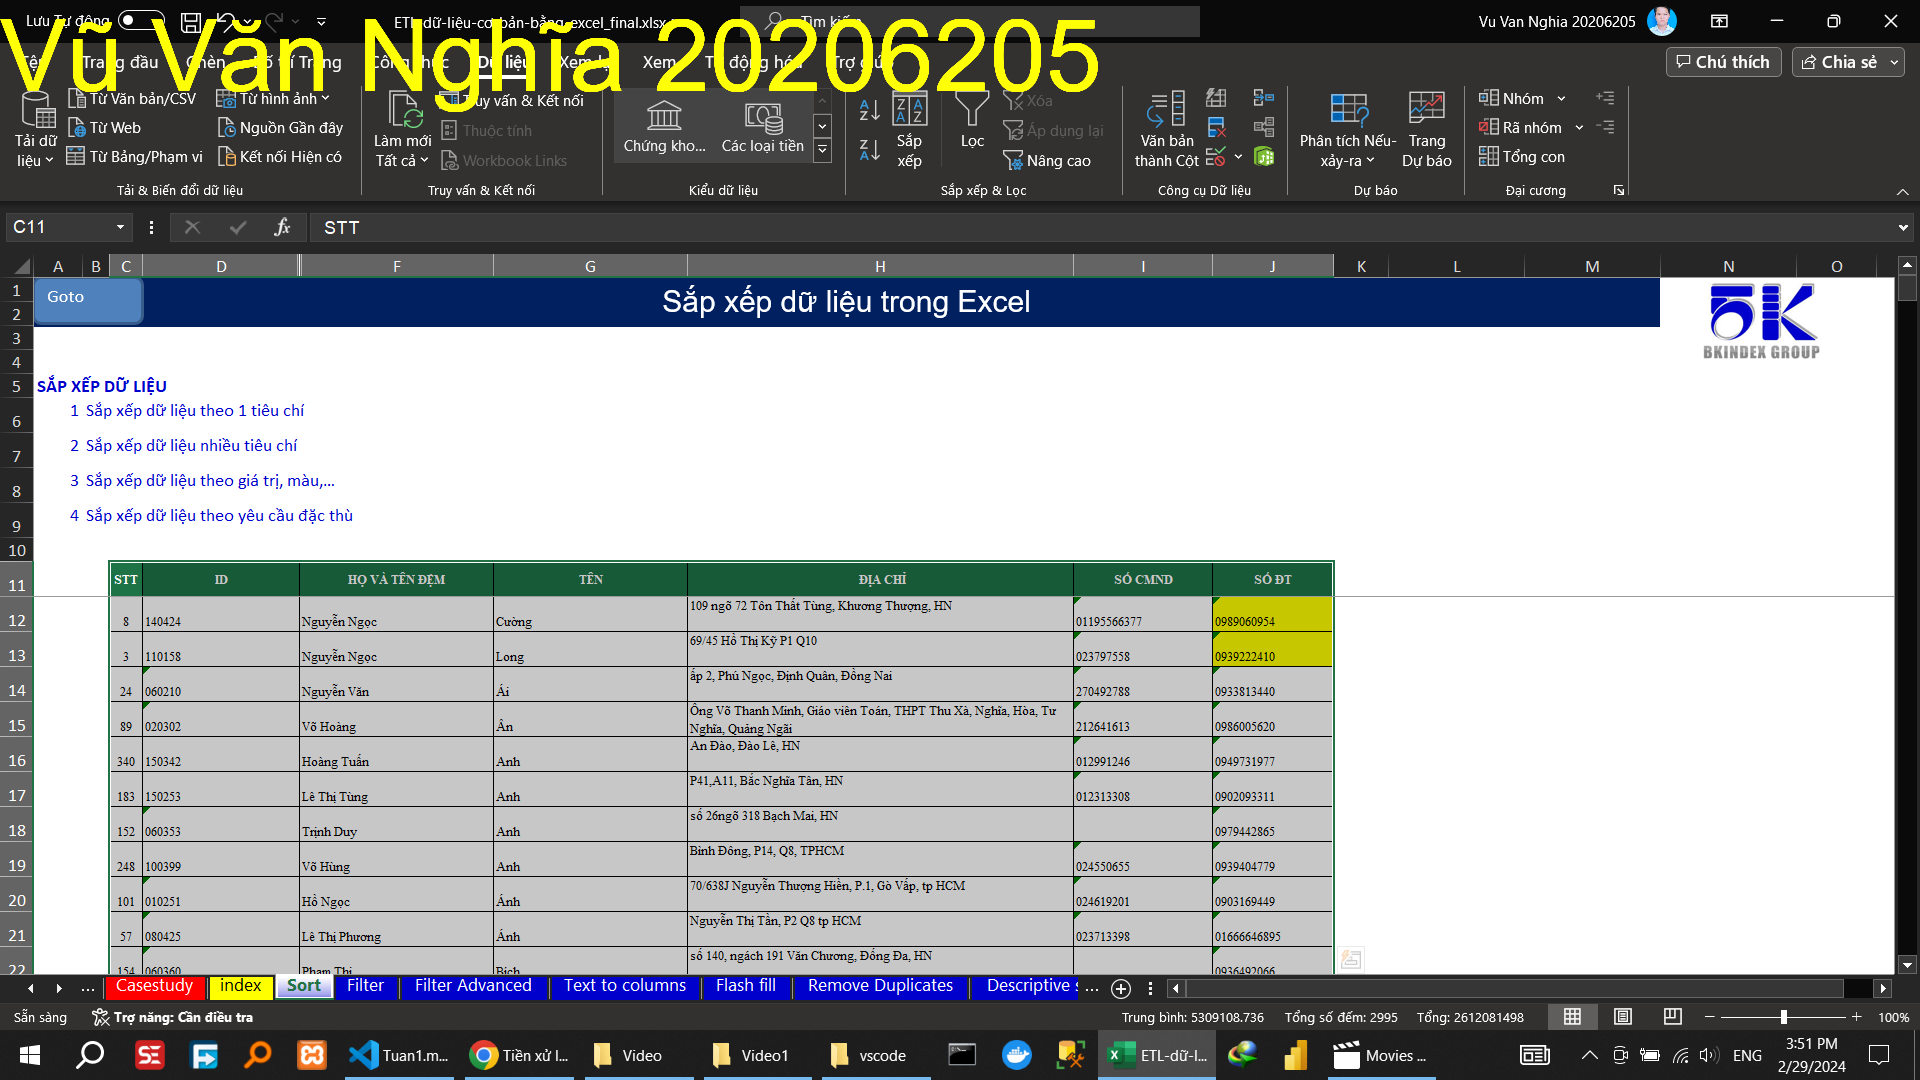
\includegraphics[scale = 0.15]{Video1/HuongDan/3.png}
\caption{Hướng dẫn sắp xếp dữ liệu theo giá trị, màu, \dots của số điện thoại}
\end{figure}

\begin{figure}[H]
\centering
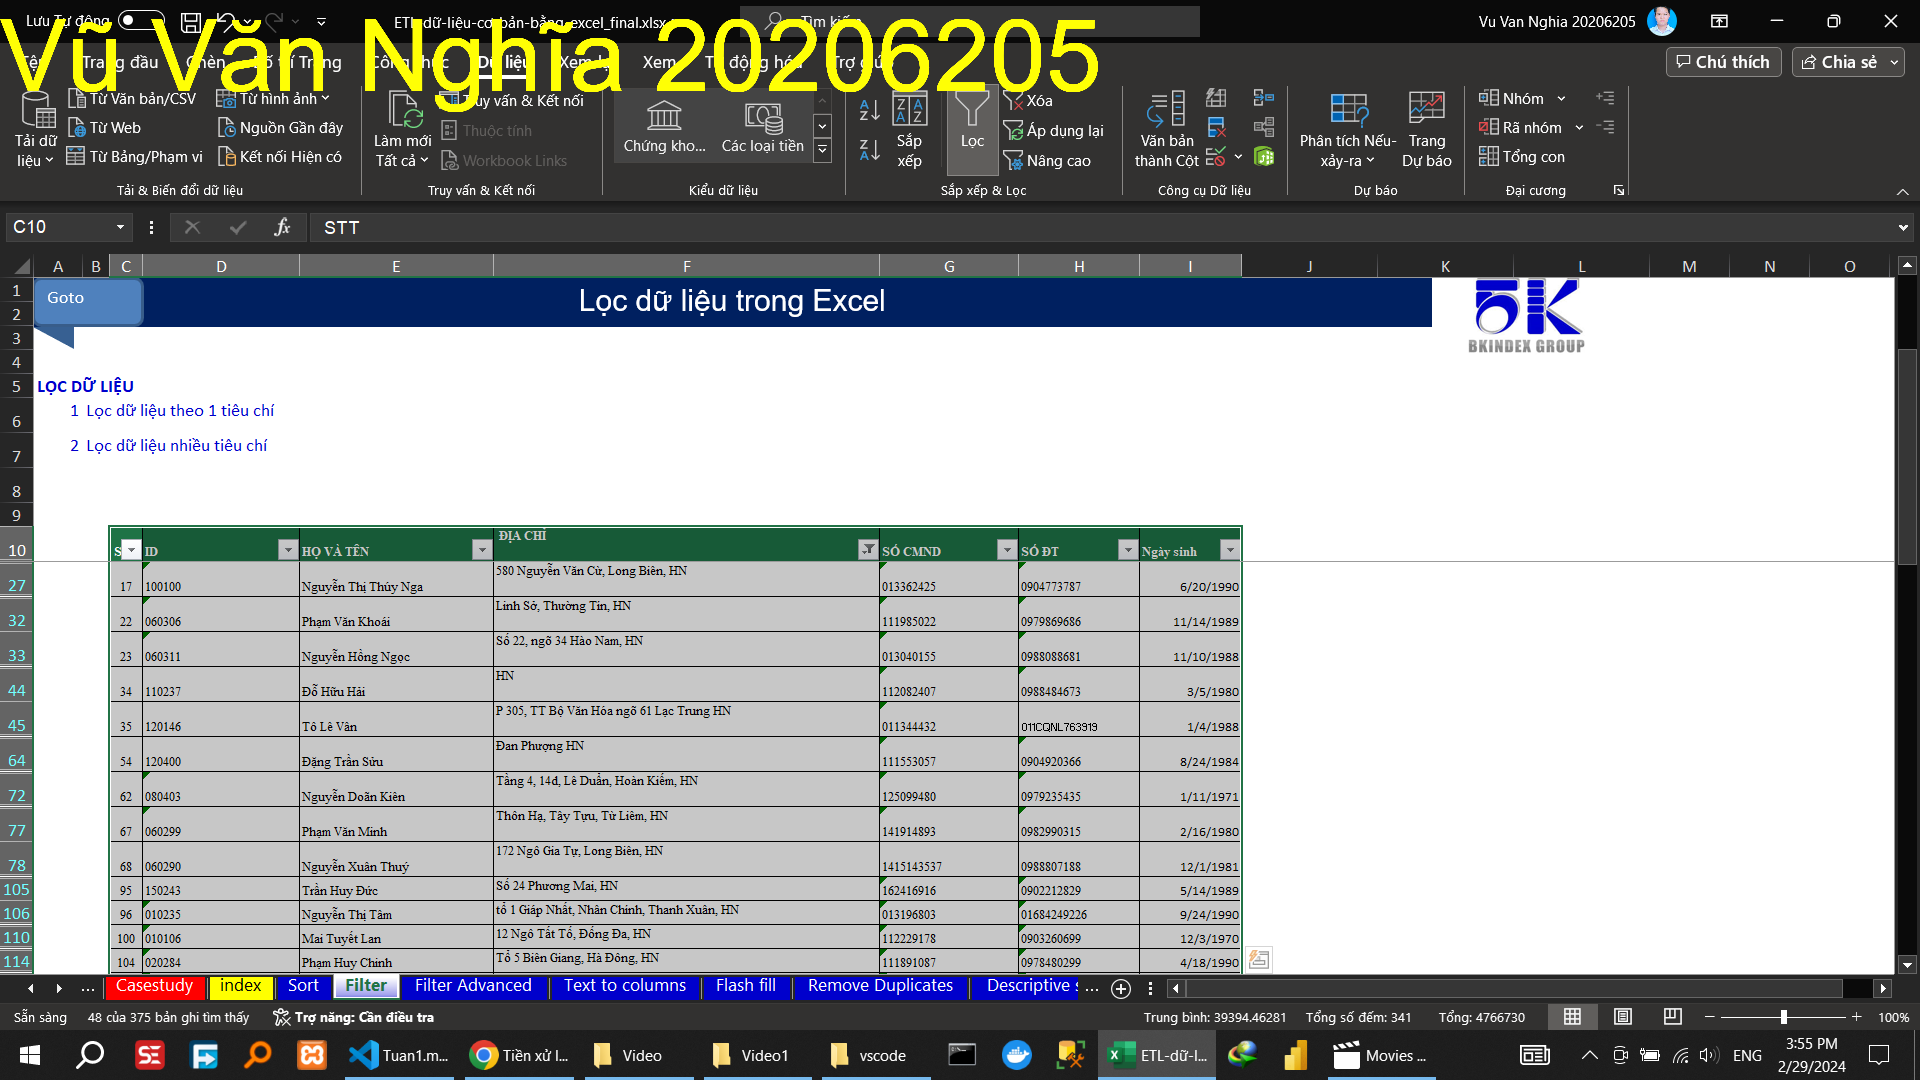
\includegraphics[scale = 0.15]{Video1/HuongDan/4.png}
\caption{Hướng dẫn lọc dữ liệu theo 1 tiêu chí là địa chỉ HN}
\end{figure}

\begin{figure}[H]
\centering
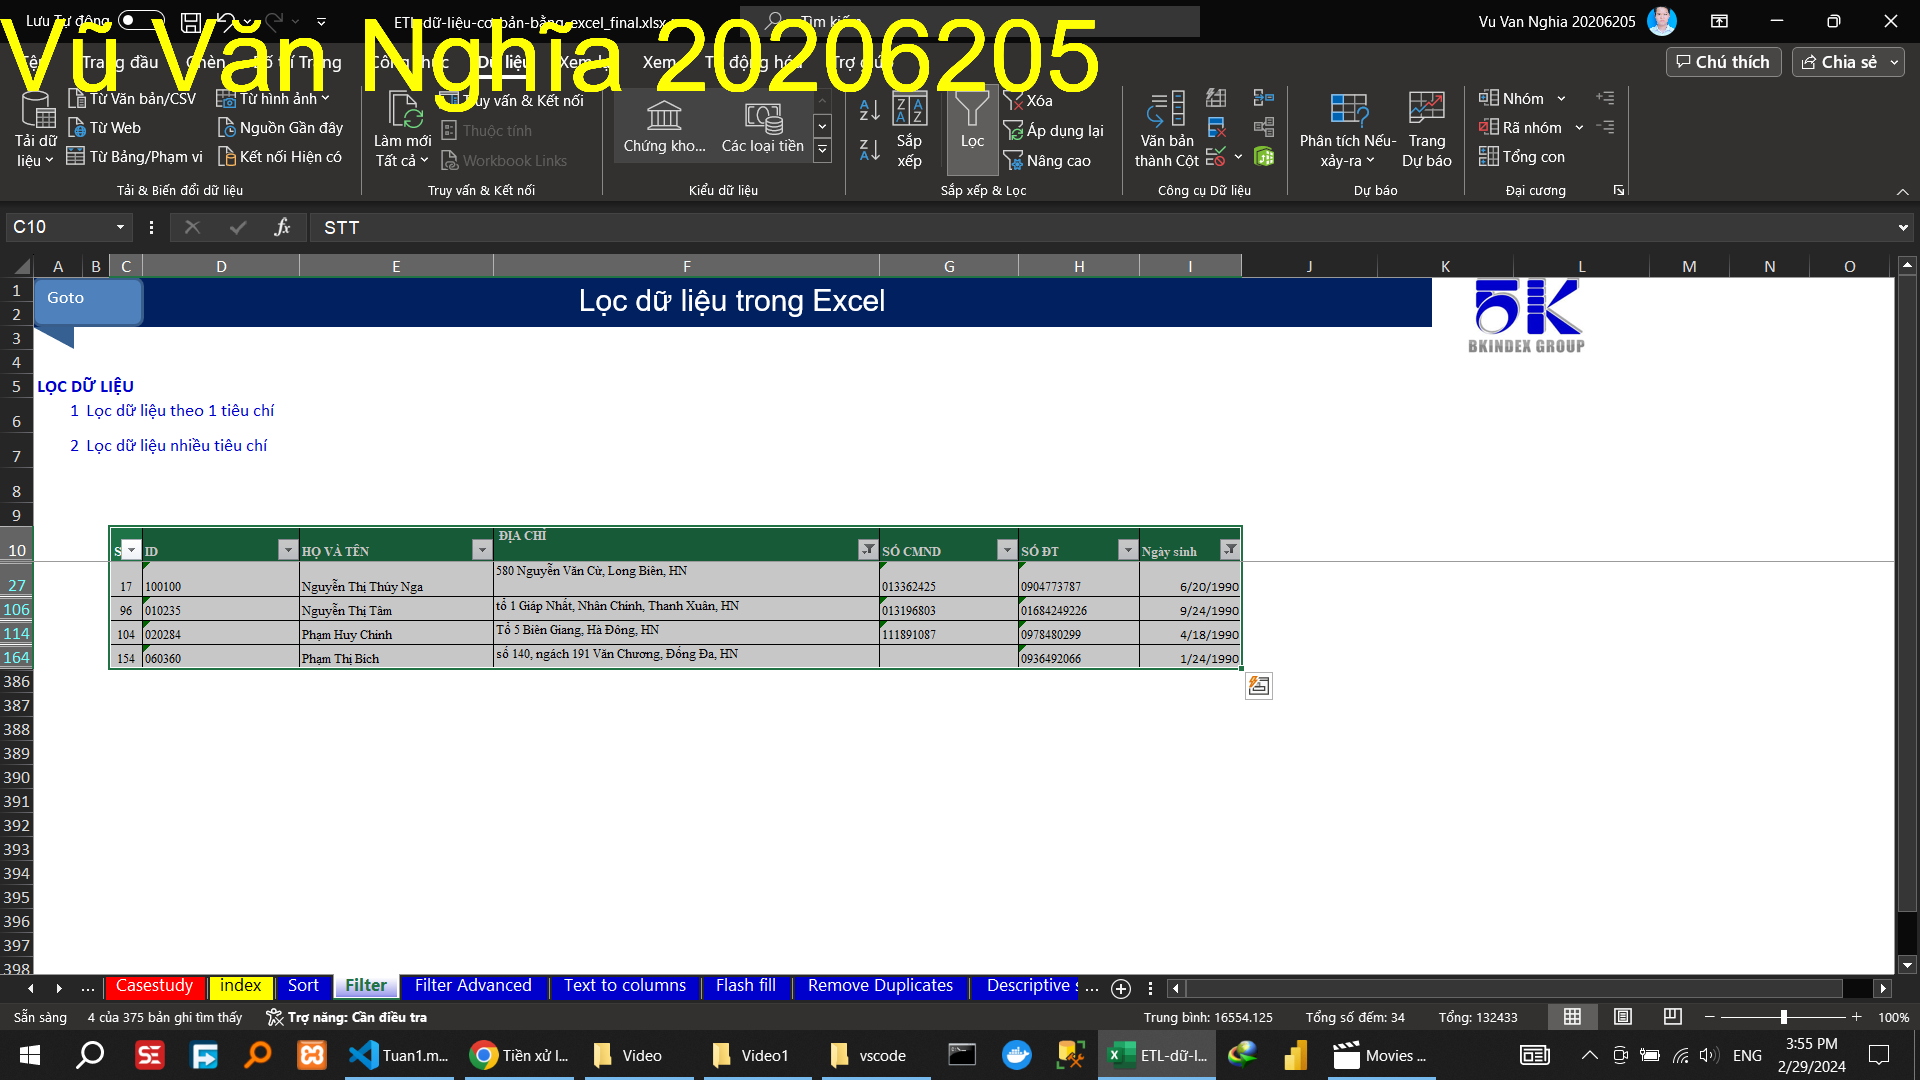
\includegraphics[scale = 0.15]{Video1/HuongDan/5.png}
\caption{Hướng dẫn lọc dữ liệu theo nhiều tiêu chí địa chỉ và sinh năm 1990}
\end{figure}

\begin{figure}[H]
\centering
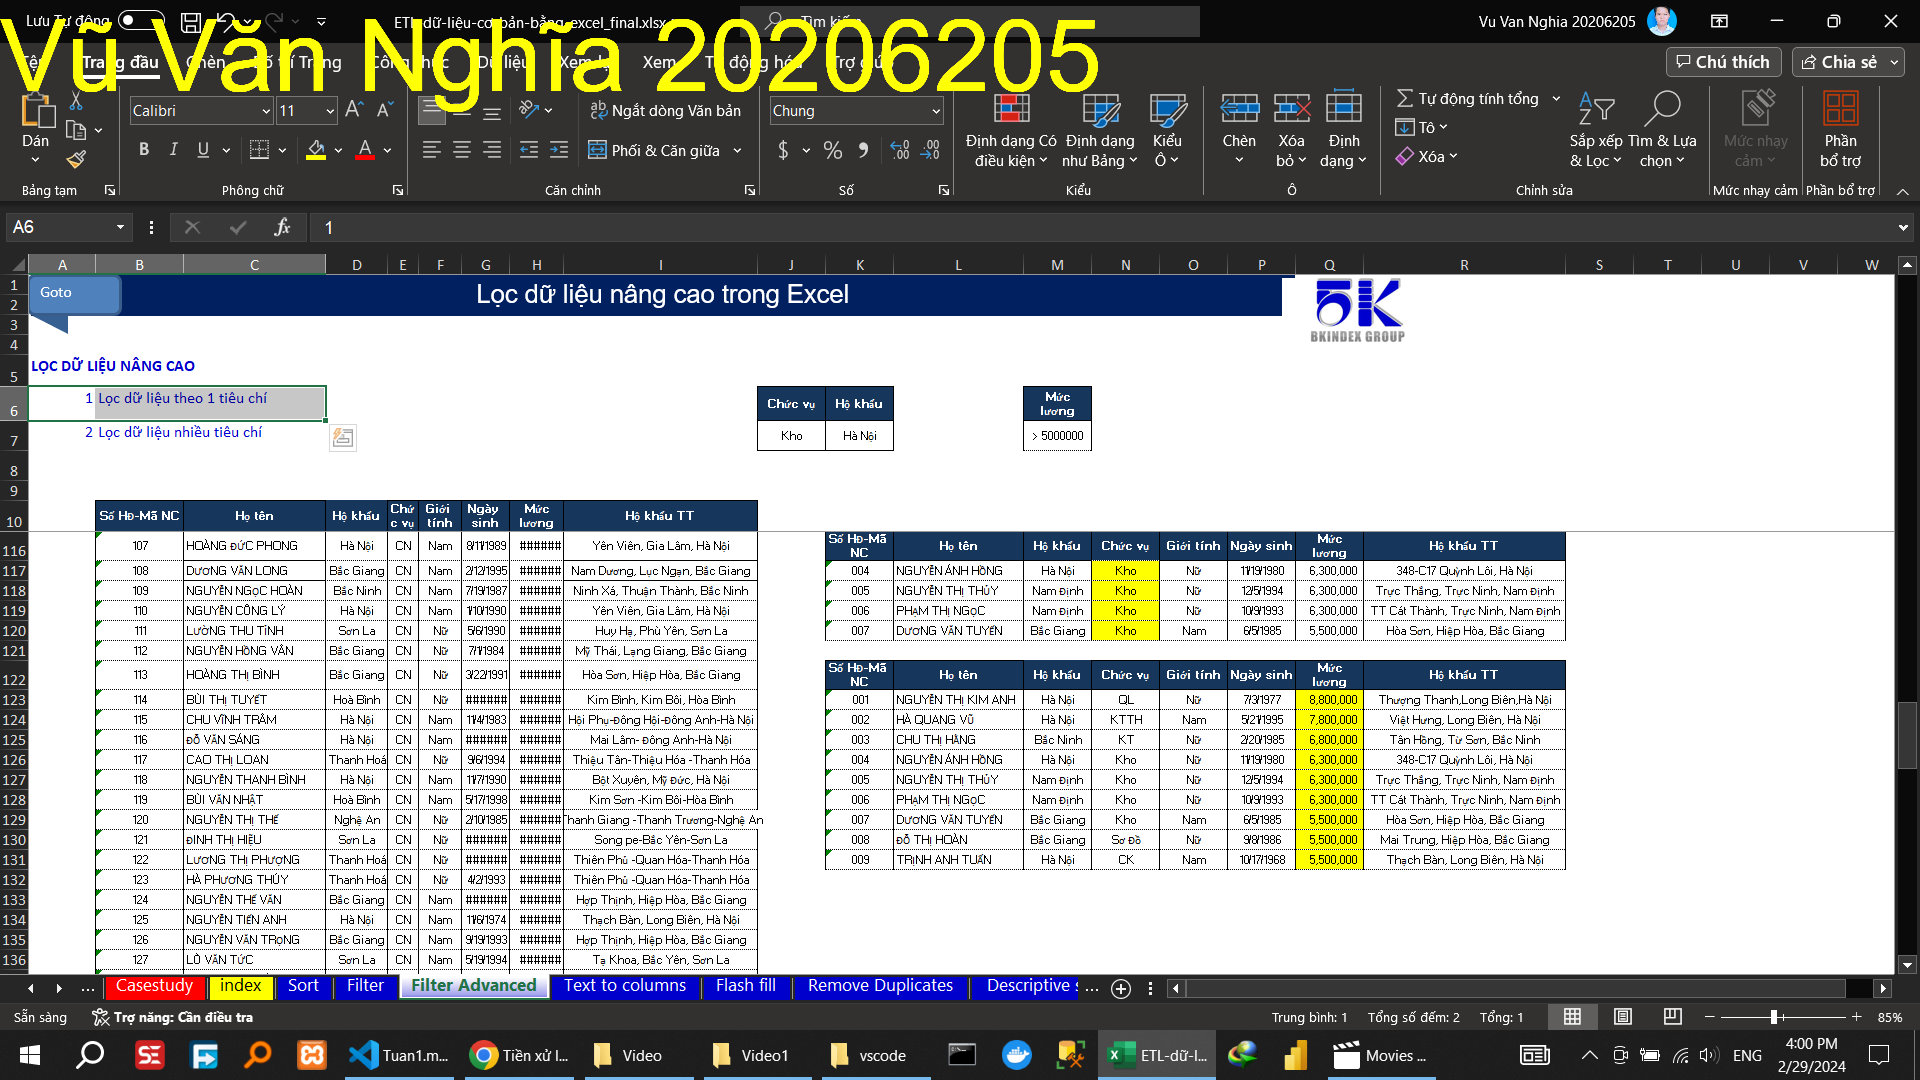
\includegraphics[scale = 0.15]{Video1/HuongDan/6.png}
\caption{Hướng dẫn lọc dữ liệu nâng cao theo 1 tiêu chí là chức vụ hoặc mức lương}
\end{figure}

\begin{figure}[H]
\centering
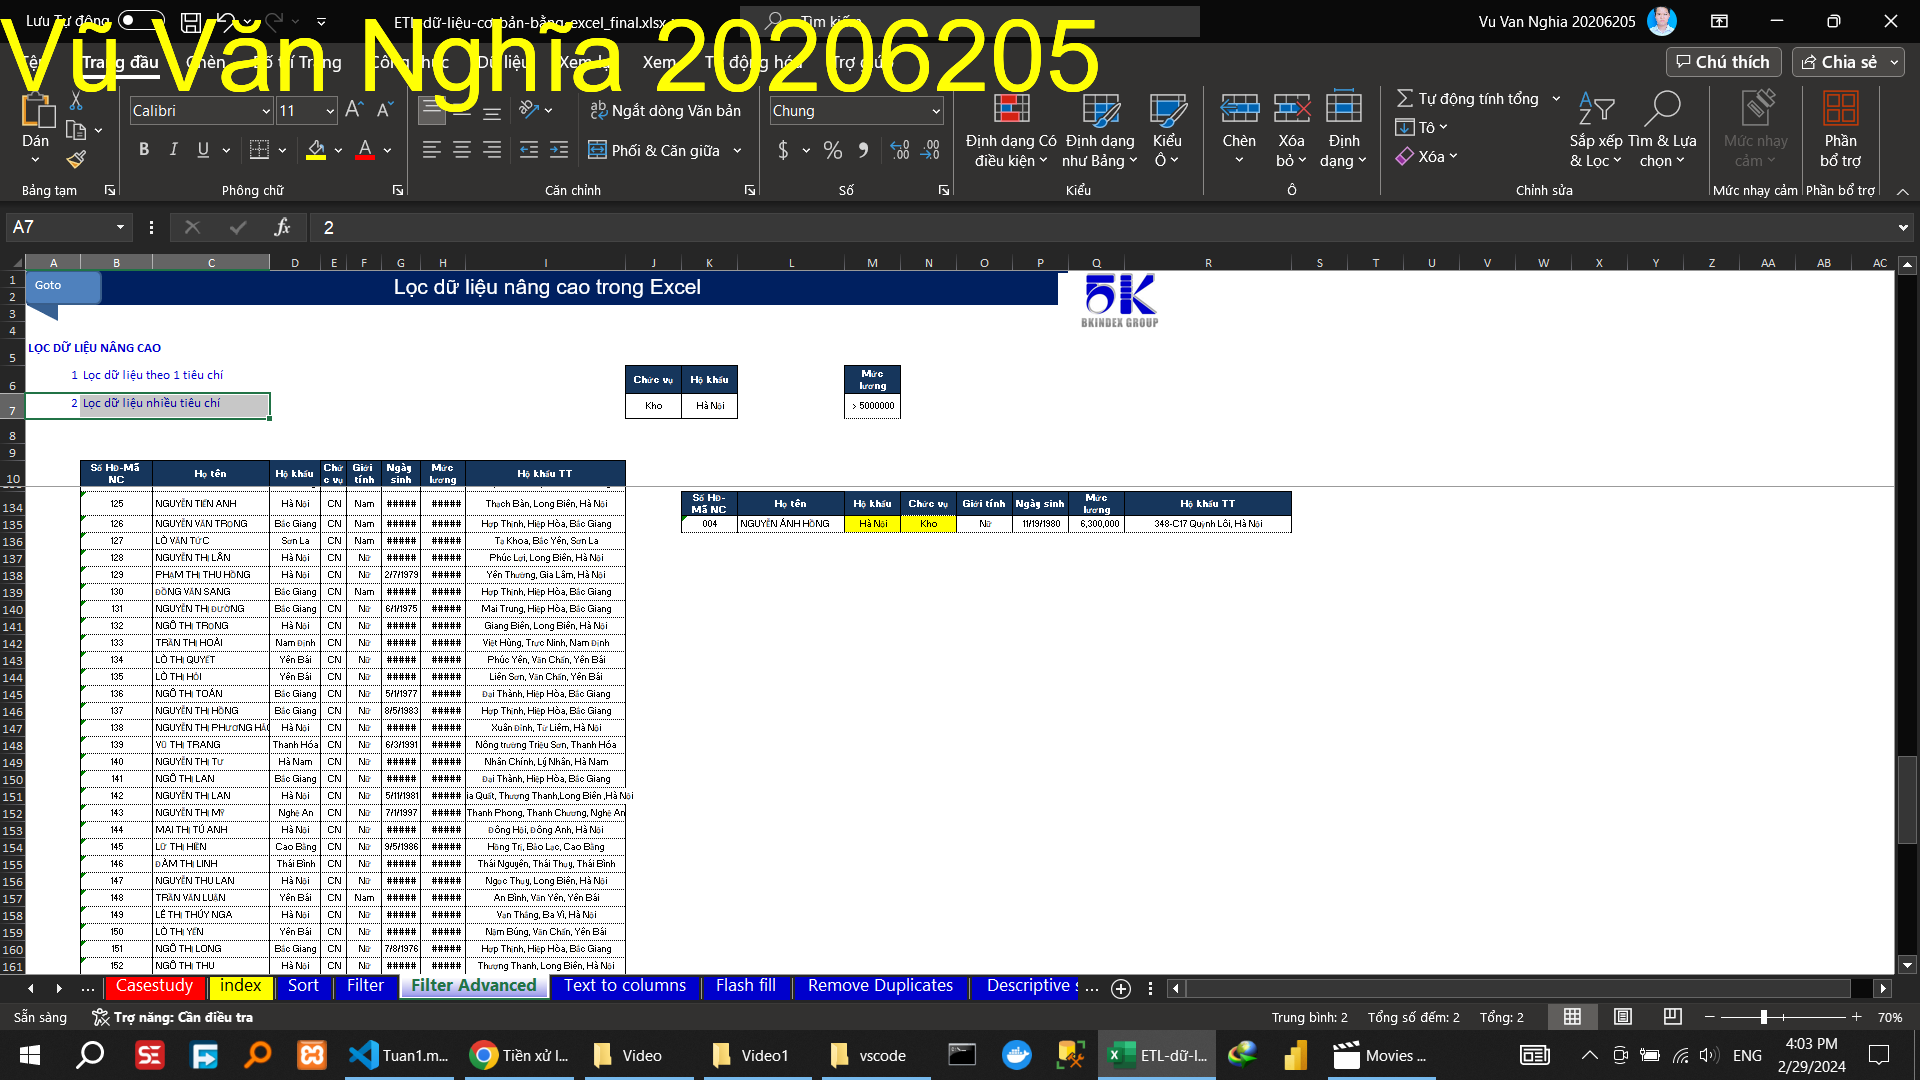
\includegraphics[scale = 0.15]{Video1/HuongDan/7.png}
\caption{Hướng dẫn lọc dữ liệu nâng cao theo nhiều tiêu chí chức vụ và hộ khẩu}
\end{figure}

\begin{figure}[H]
\centering
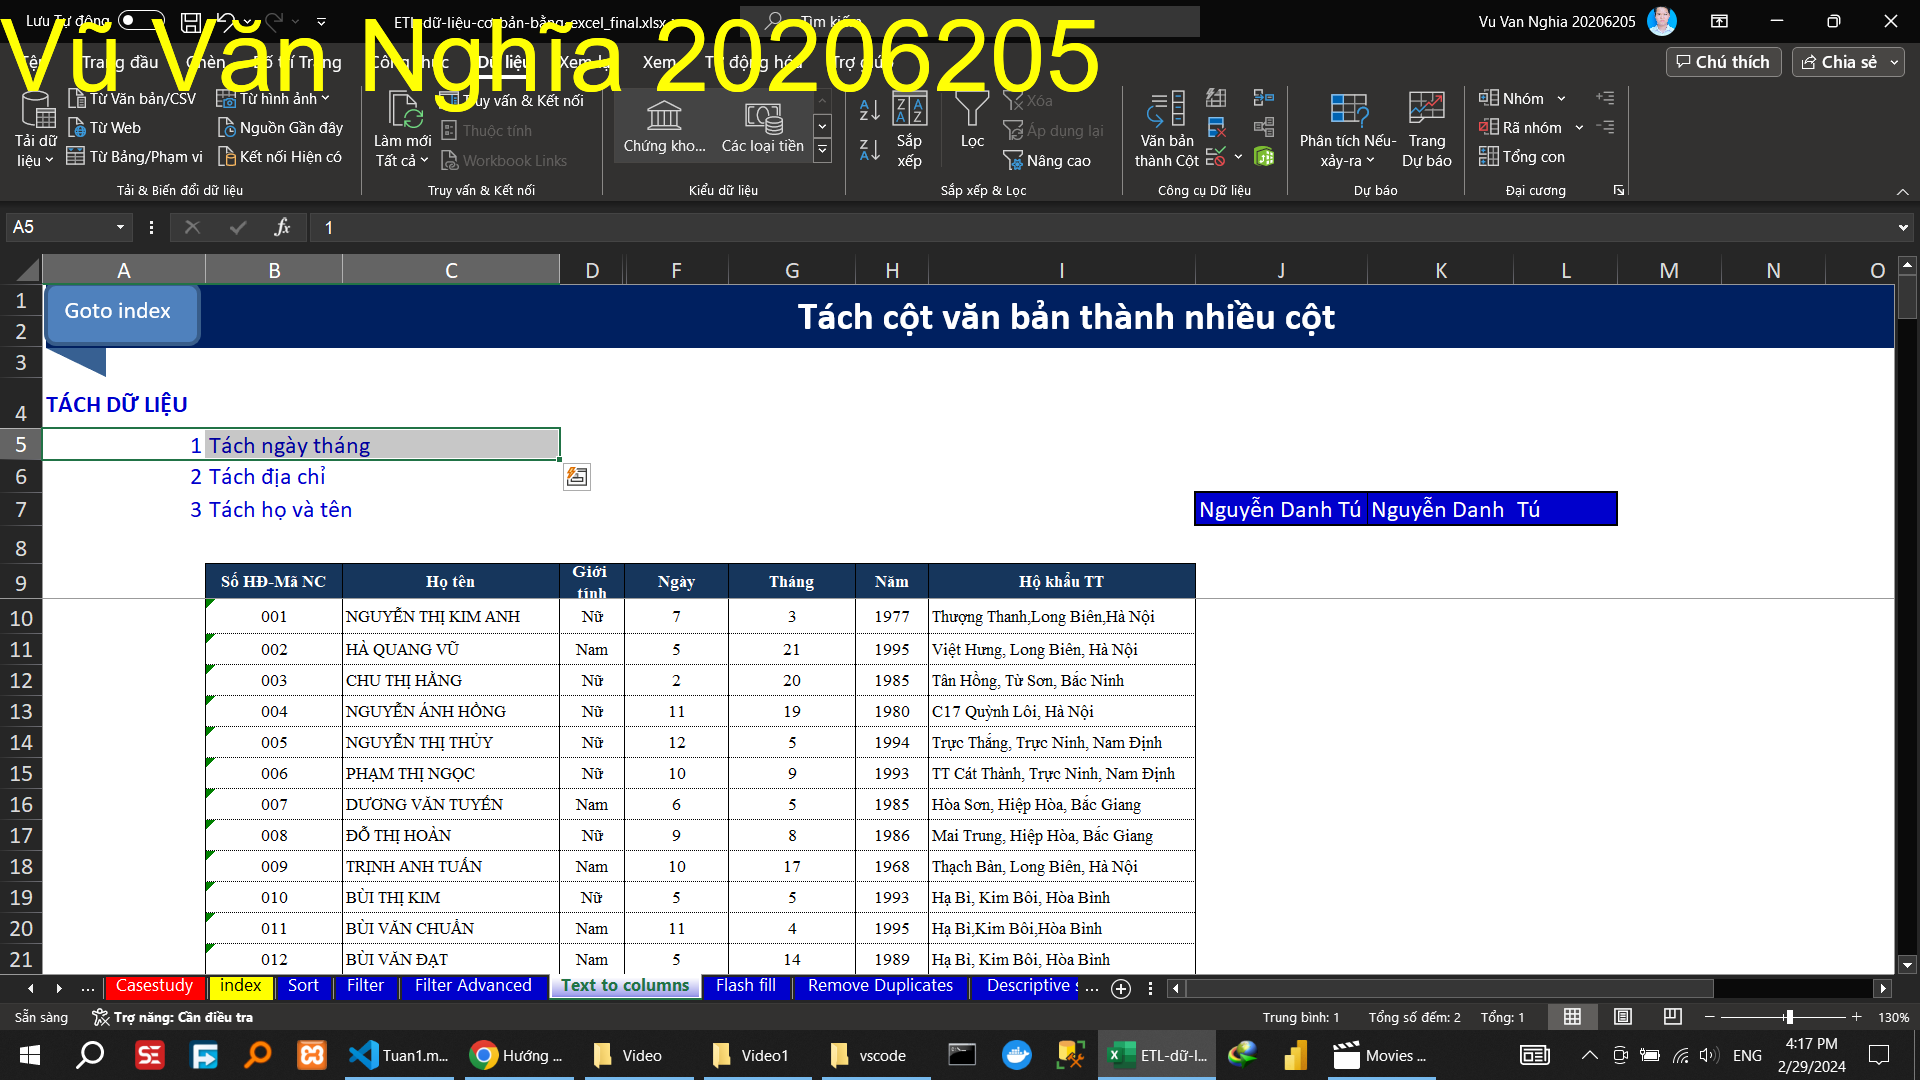
\includegraphics[scale = 0.15]{Video1/HuongDan/8.png}
\caption{Hướng dẫn tách ngày tháng}
\end{figure}

\begin{figure}[H]
\centering
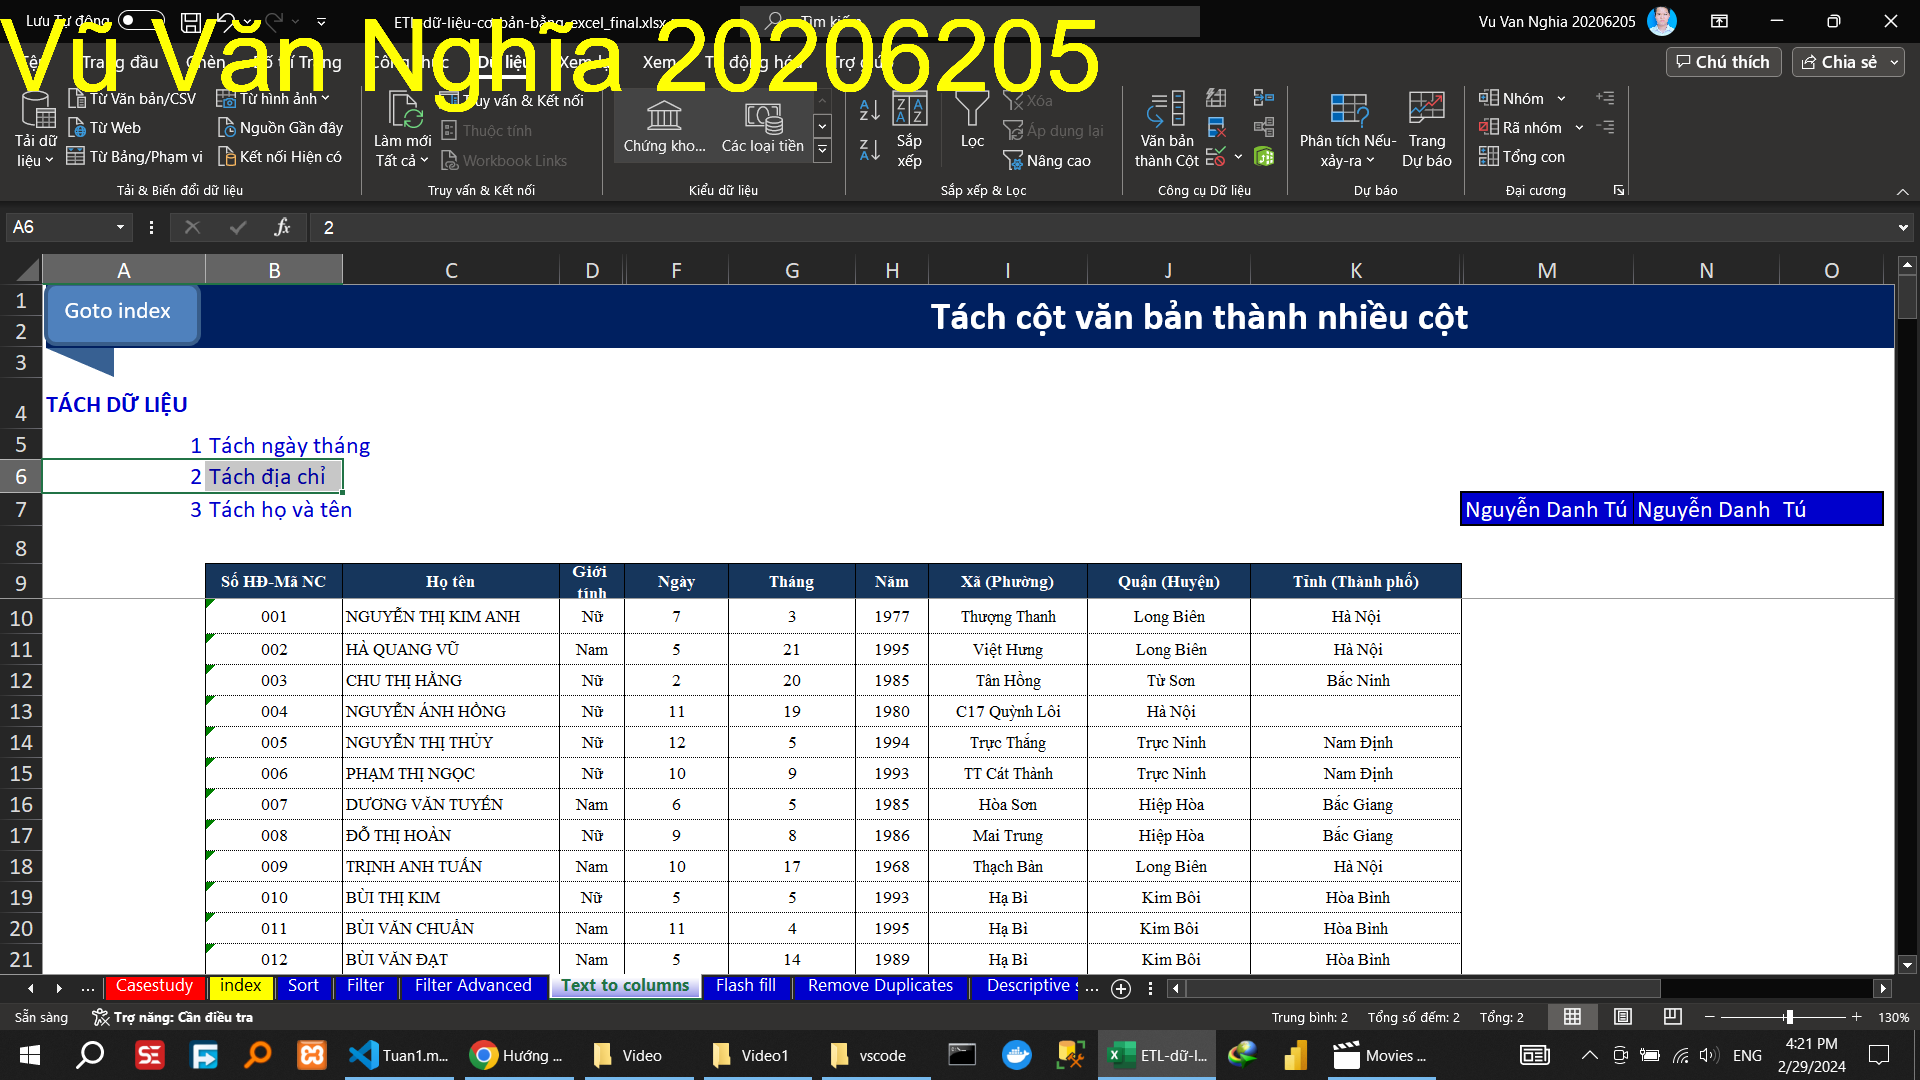
\includegraphics[scale = 0.15]{Video1/HuongDan/9.png}
\caption{Hướng dẫn tách địa chỉ}
\end{figure}

\begin{figure}[H]
\centering
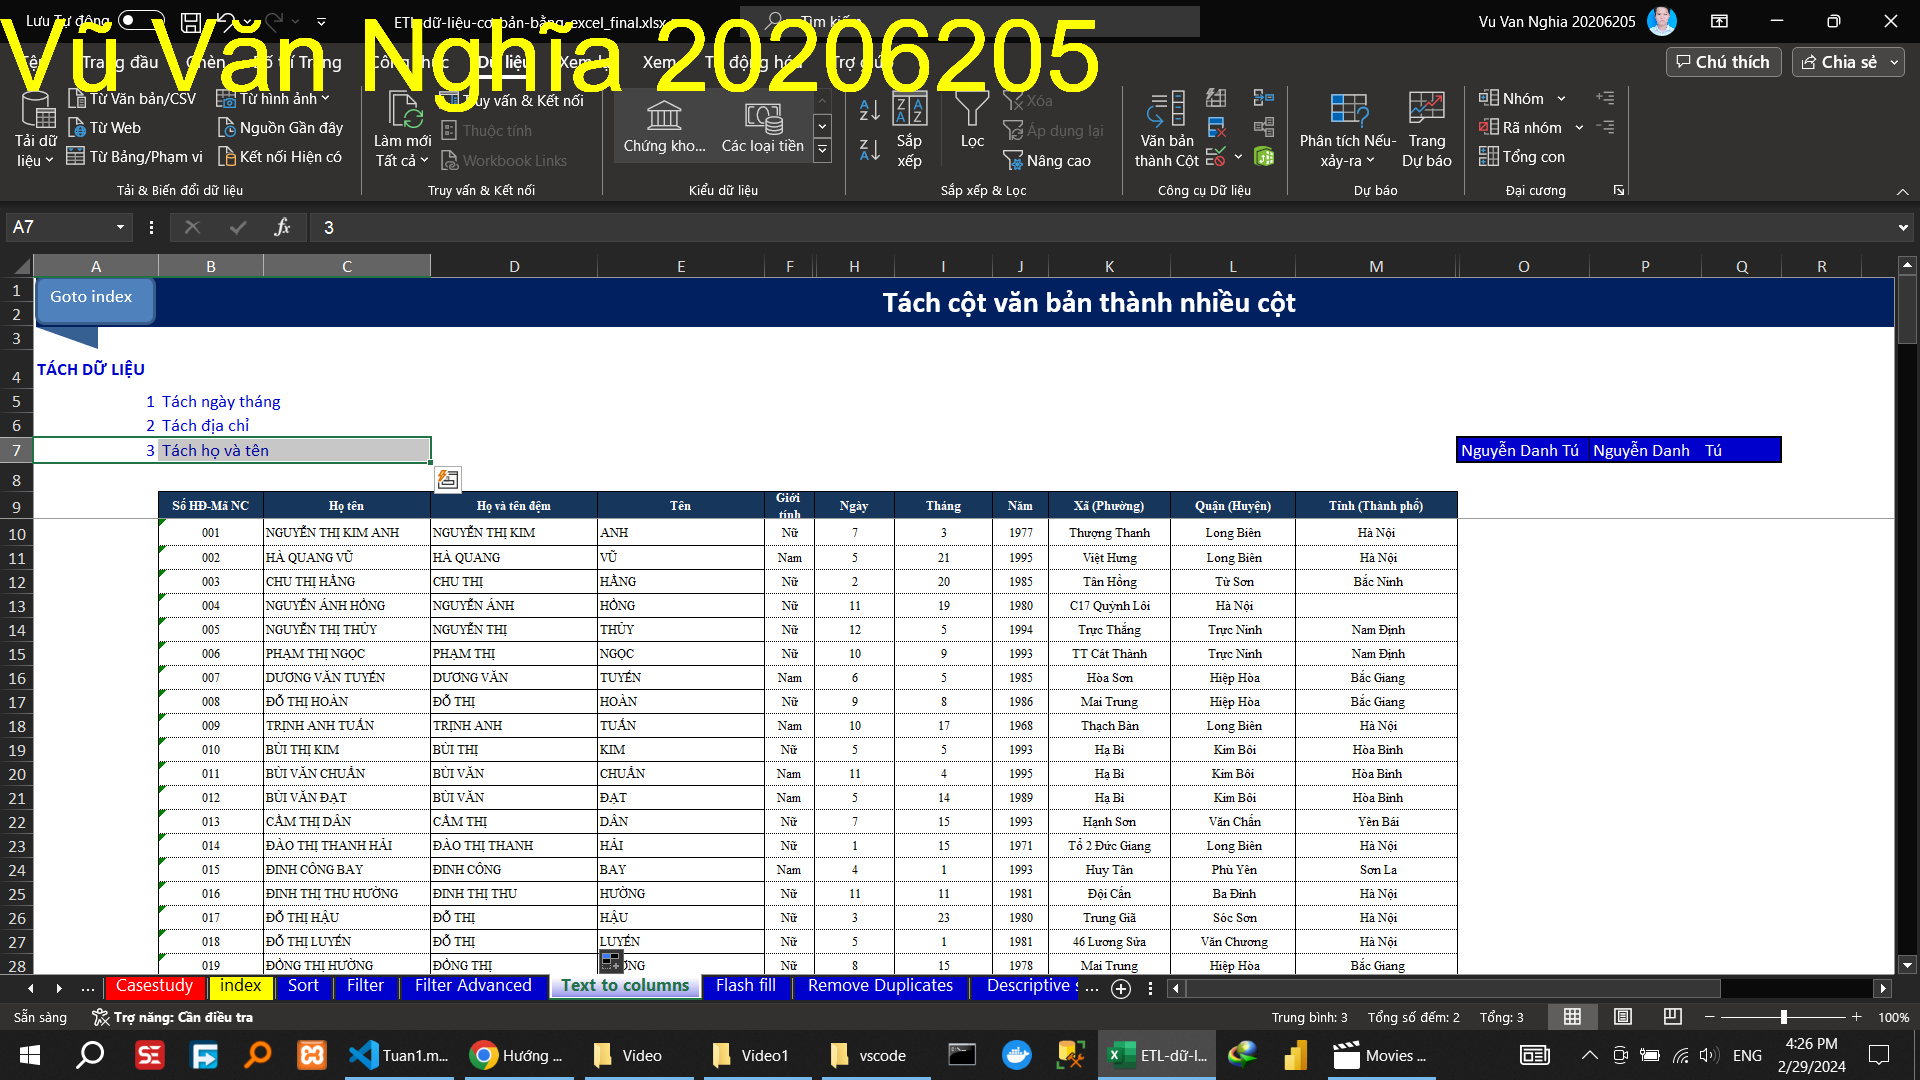
\includegraphics[scale = 0.15]{Video1/HuongDan/10.png}
\caption{Hướng dẫn tách họ và tên}
\end{figure}

\begin{figure}[H]
\centering
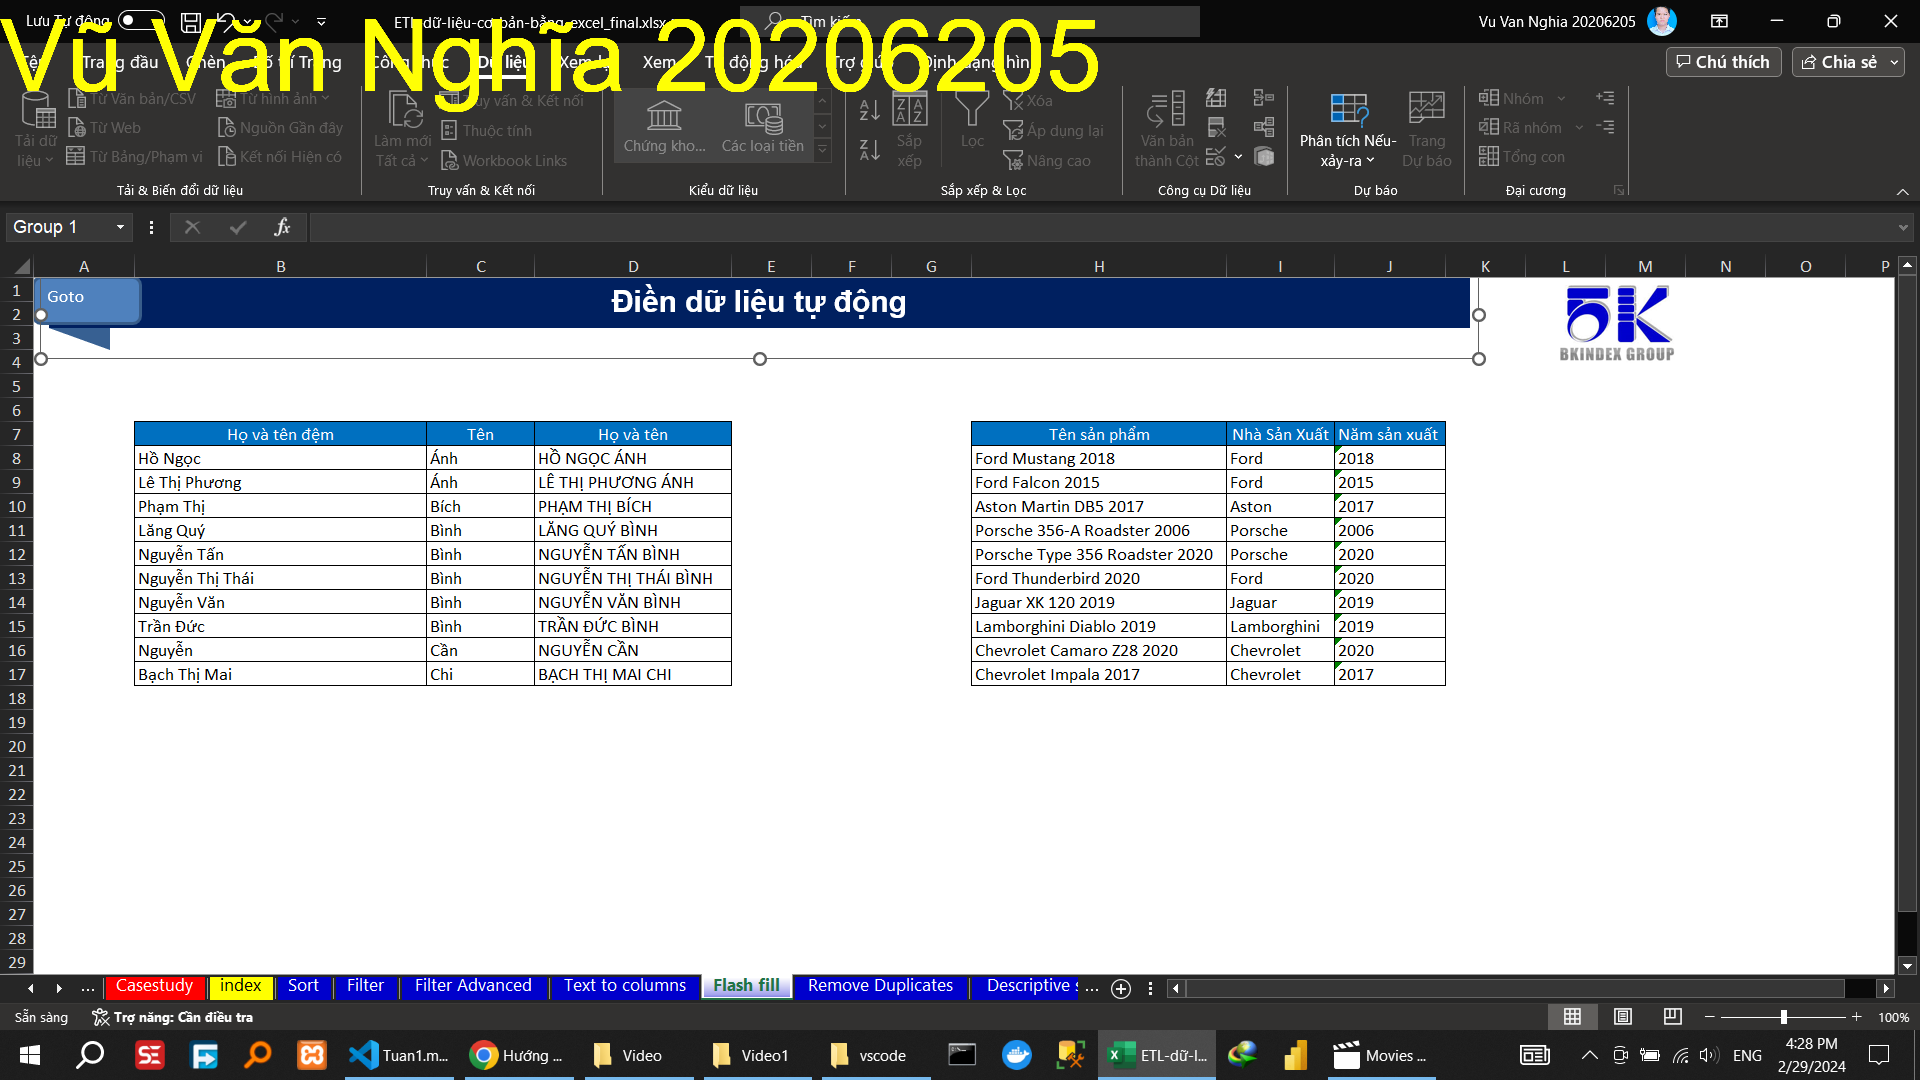
\includegraphics[scale = 0.15]{Video1/HuongDan/11.png}
\caption{Hướng dẫn điền dữ liệu tự động}
\end{figure}

\begin{figure}[H]
\centering
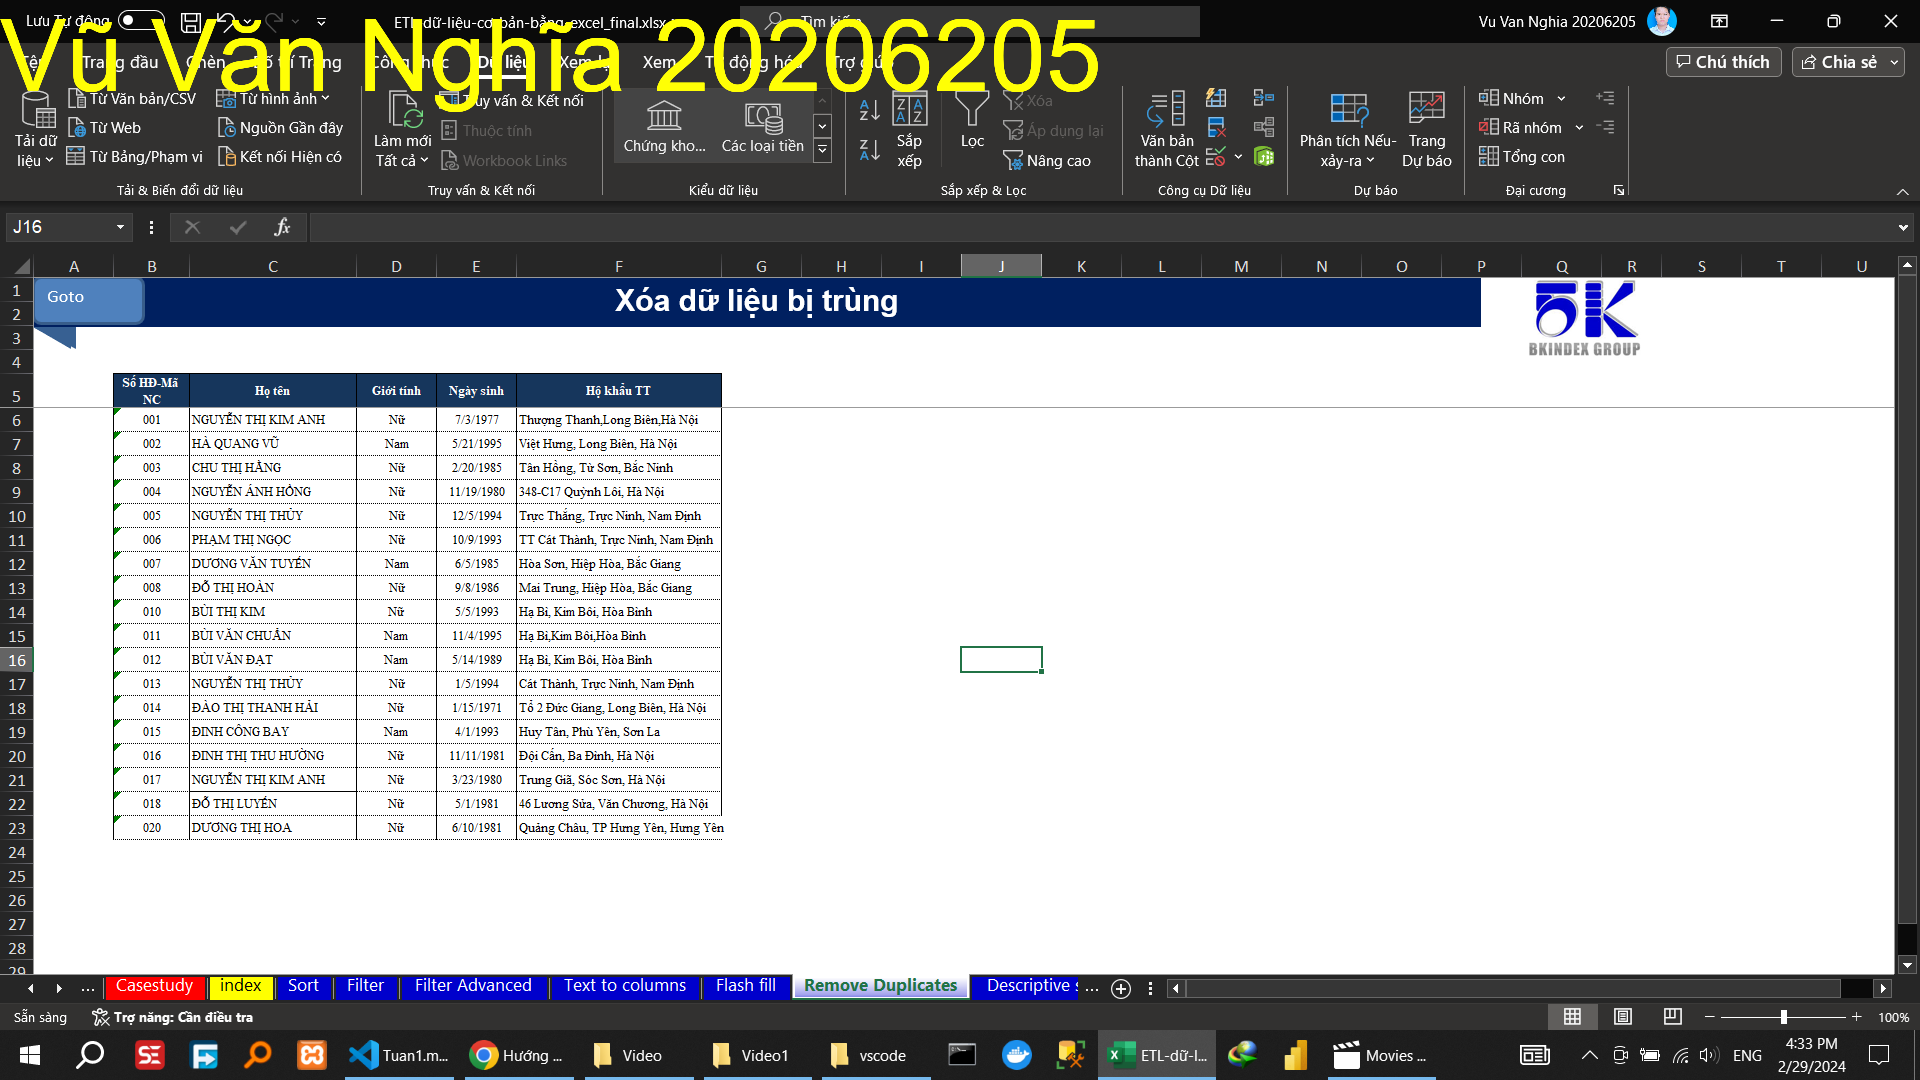
\includegraphics[scale = 0.15]{Video1/HuongDan/12.png}
\caption{Hướng dẫn xóa dữ liệu bị trùng}
\end{figure}

\begin{figure}[H]
\centering
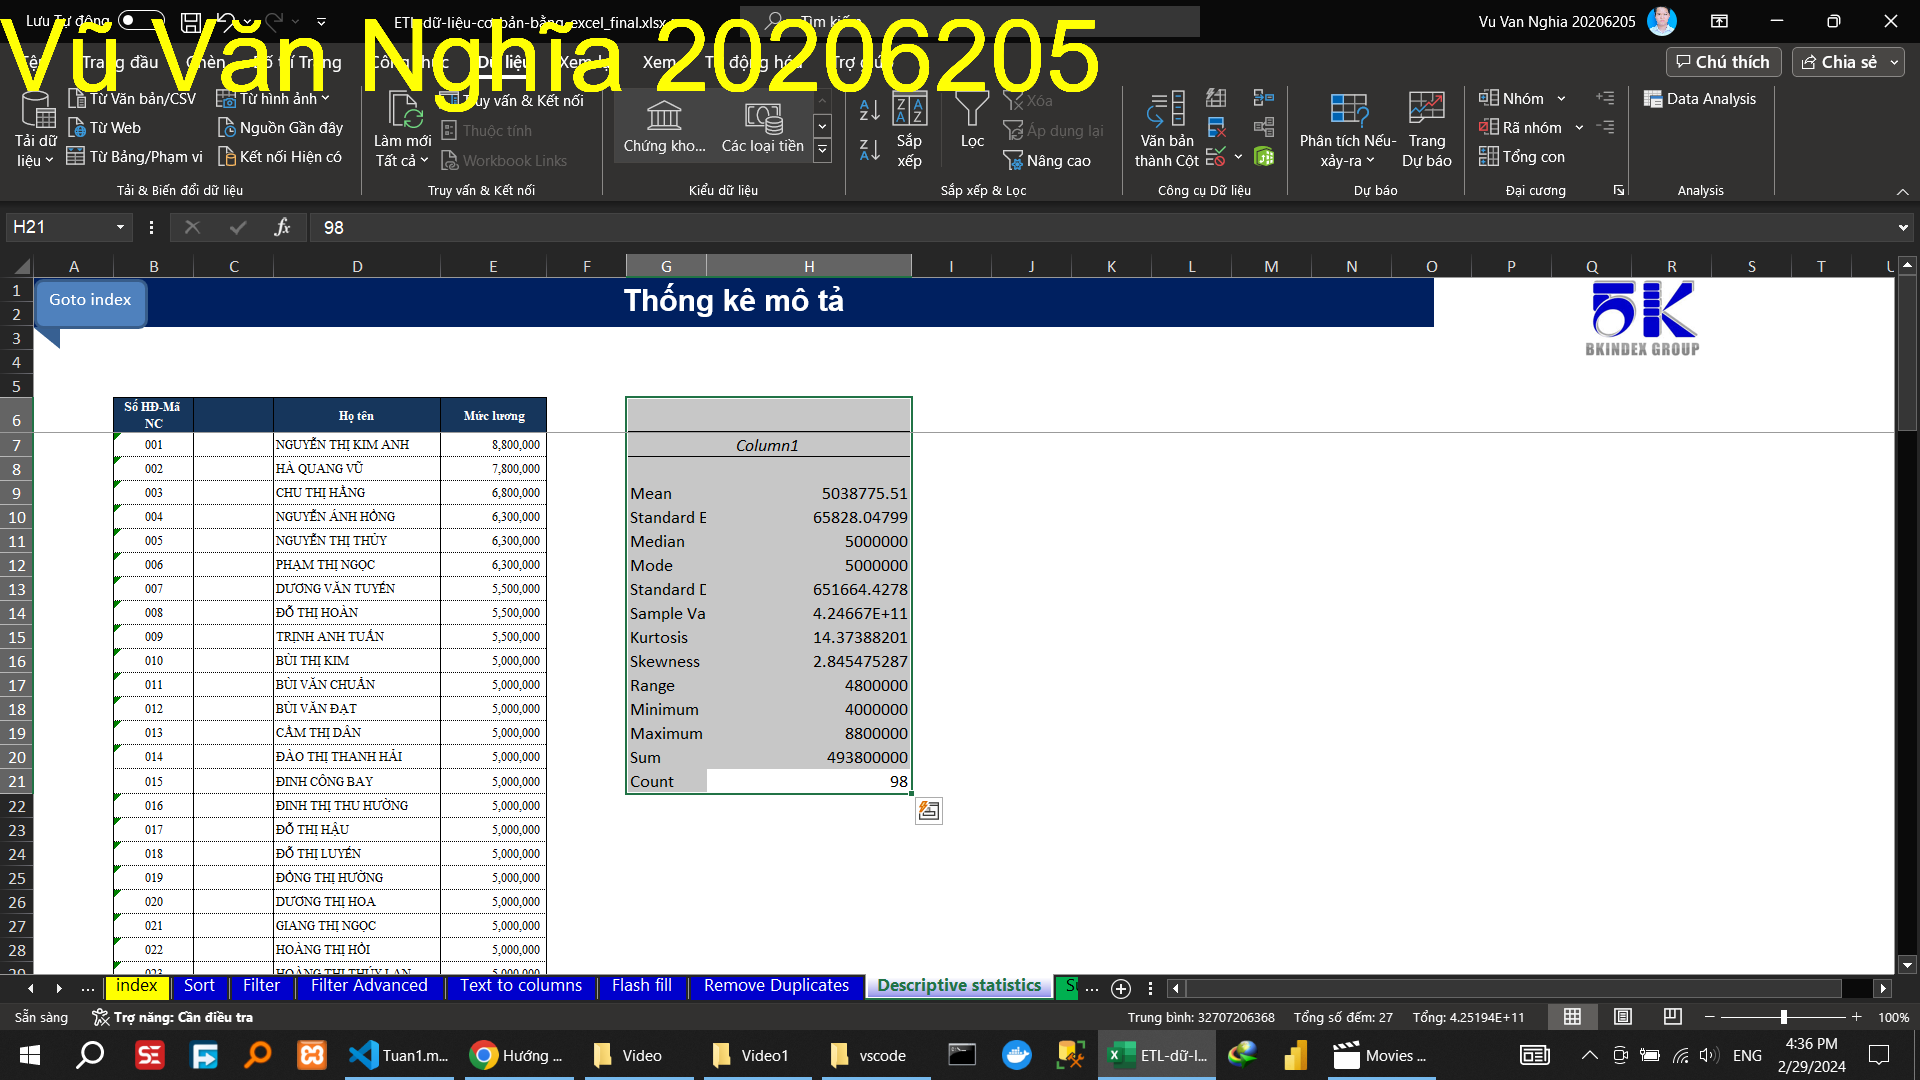
\includegraphics[scale = 0.15]{Video1/HuongDan/13.png}
\caption{Hướng dẫn thống kê mô tả}
\end{figure}
%%%%%%%%%%%%%%%%%%%%%%%%%%%%%%%%%%%%%%%%%%%%%%%%%%%%%%%
\begin{figure}[H]
\centering
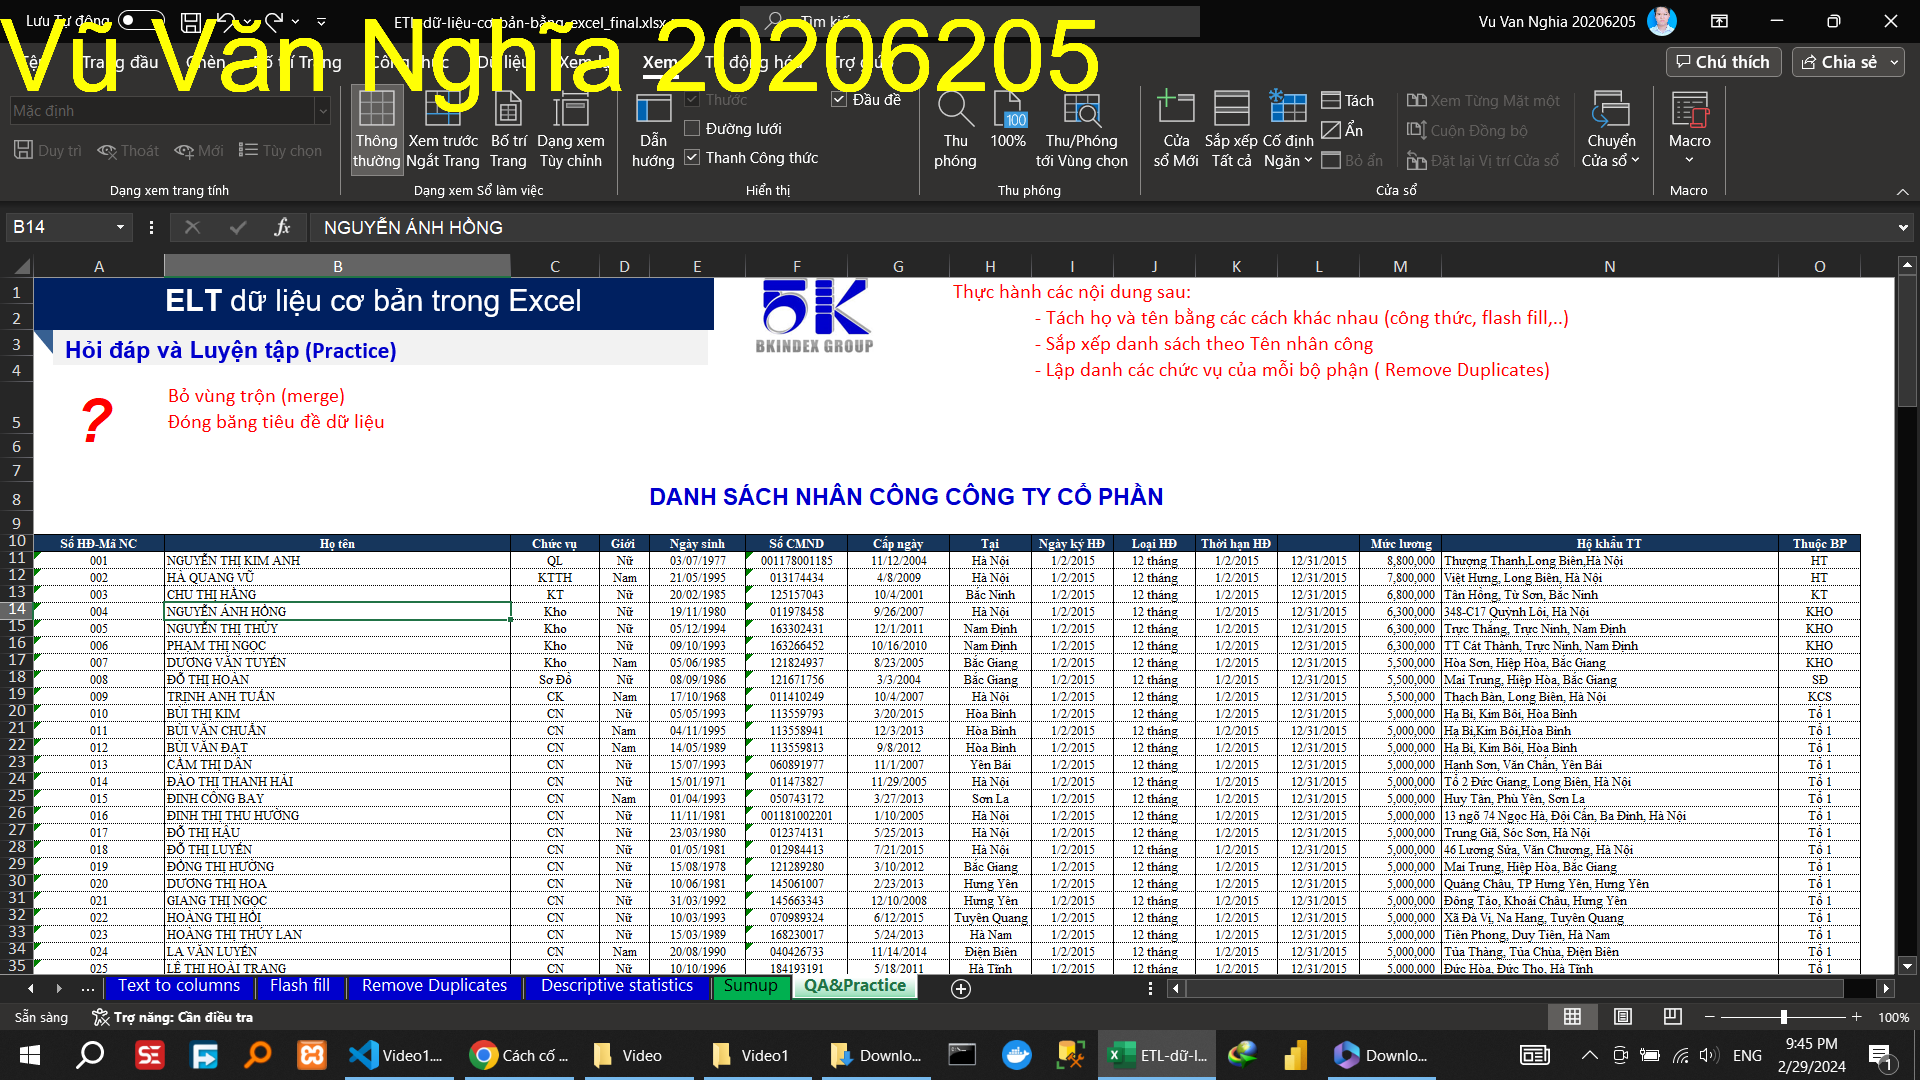
\includegraphics[scale = 0.15]{Video1/ThucHanh/1.png}
\caption{Thực hành bỏ vùng trộn (merge)}
\end{figure}

\begin{figure}[H]
\centering
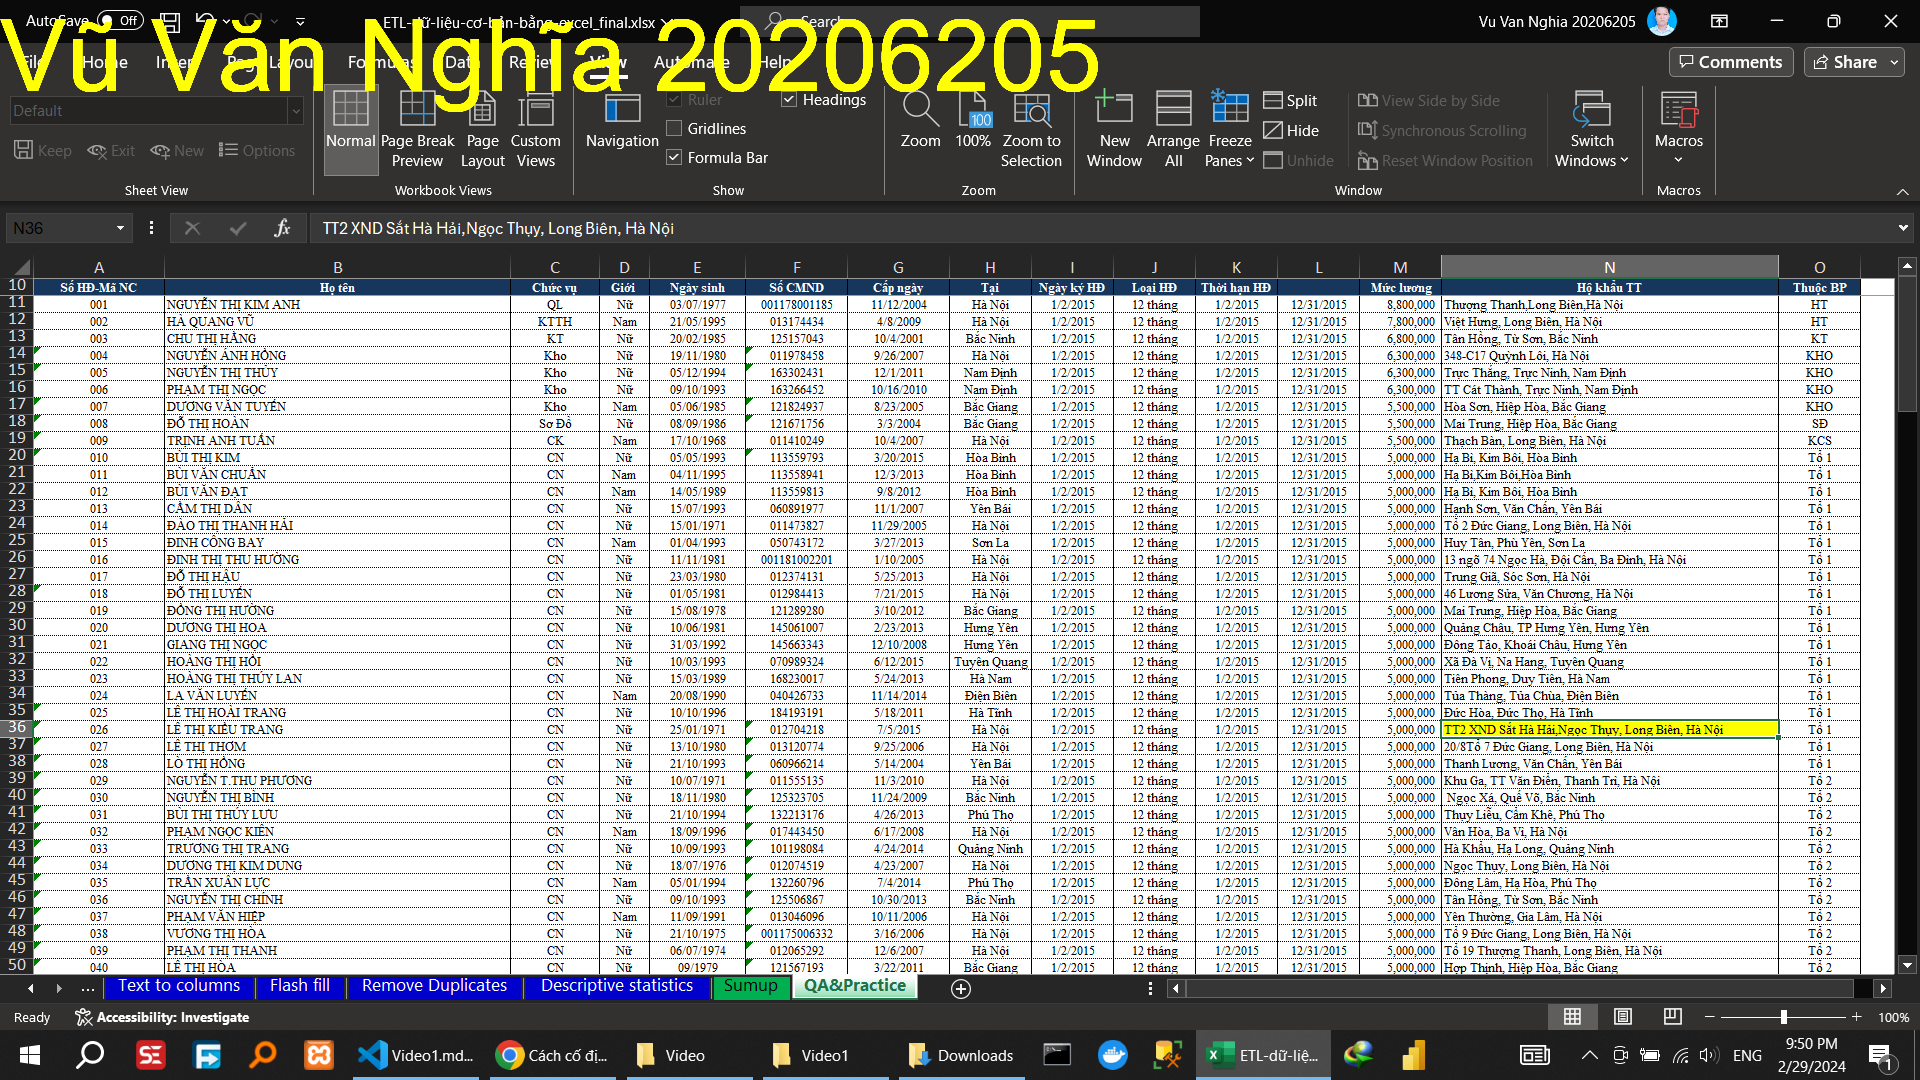
\includegraphics[scale = 0.15]{Video1/ThucHanh/2.png}
\caption{Thực hành đóng băng tiêu đề dữ liệu}
\end{figure}

\begin{figure}[H]
\centering
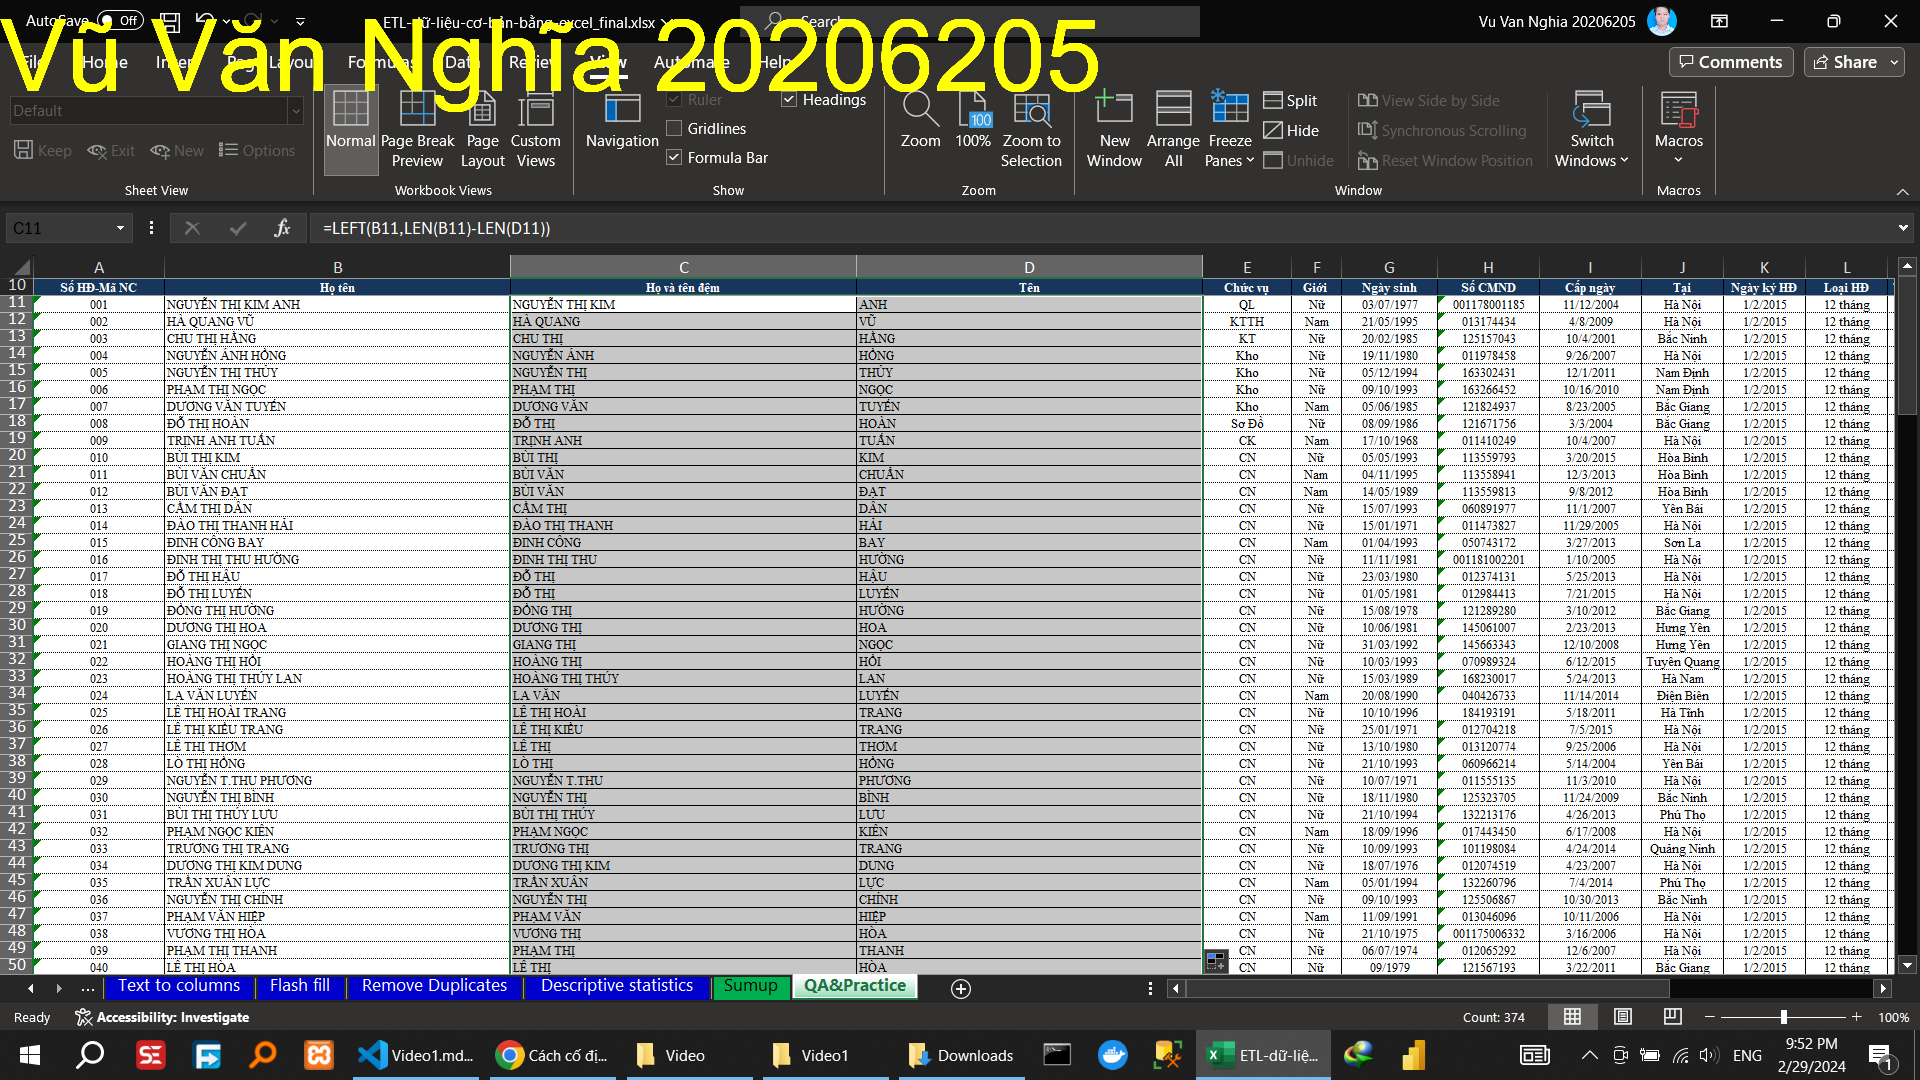
\includegraphics[scale = 0.15]{Video1/ThucHanh/3.png}
\caption{Thực hành tách họ và tên bằng công thức}
\end{figure}

\begin{figure}[H]
\centering
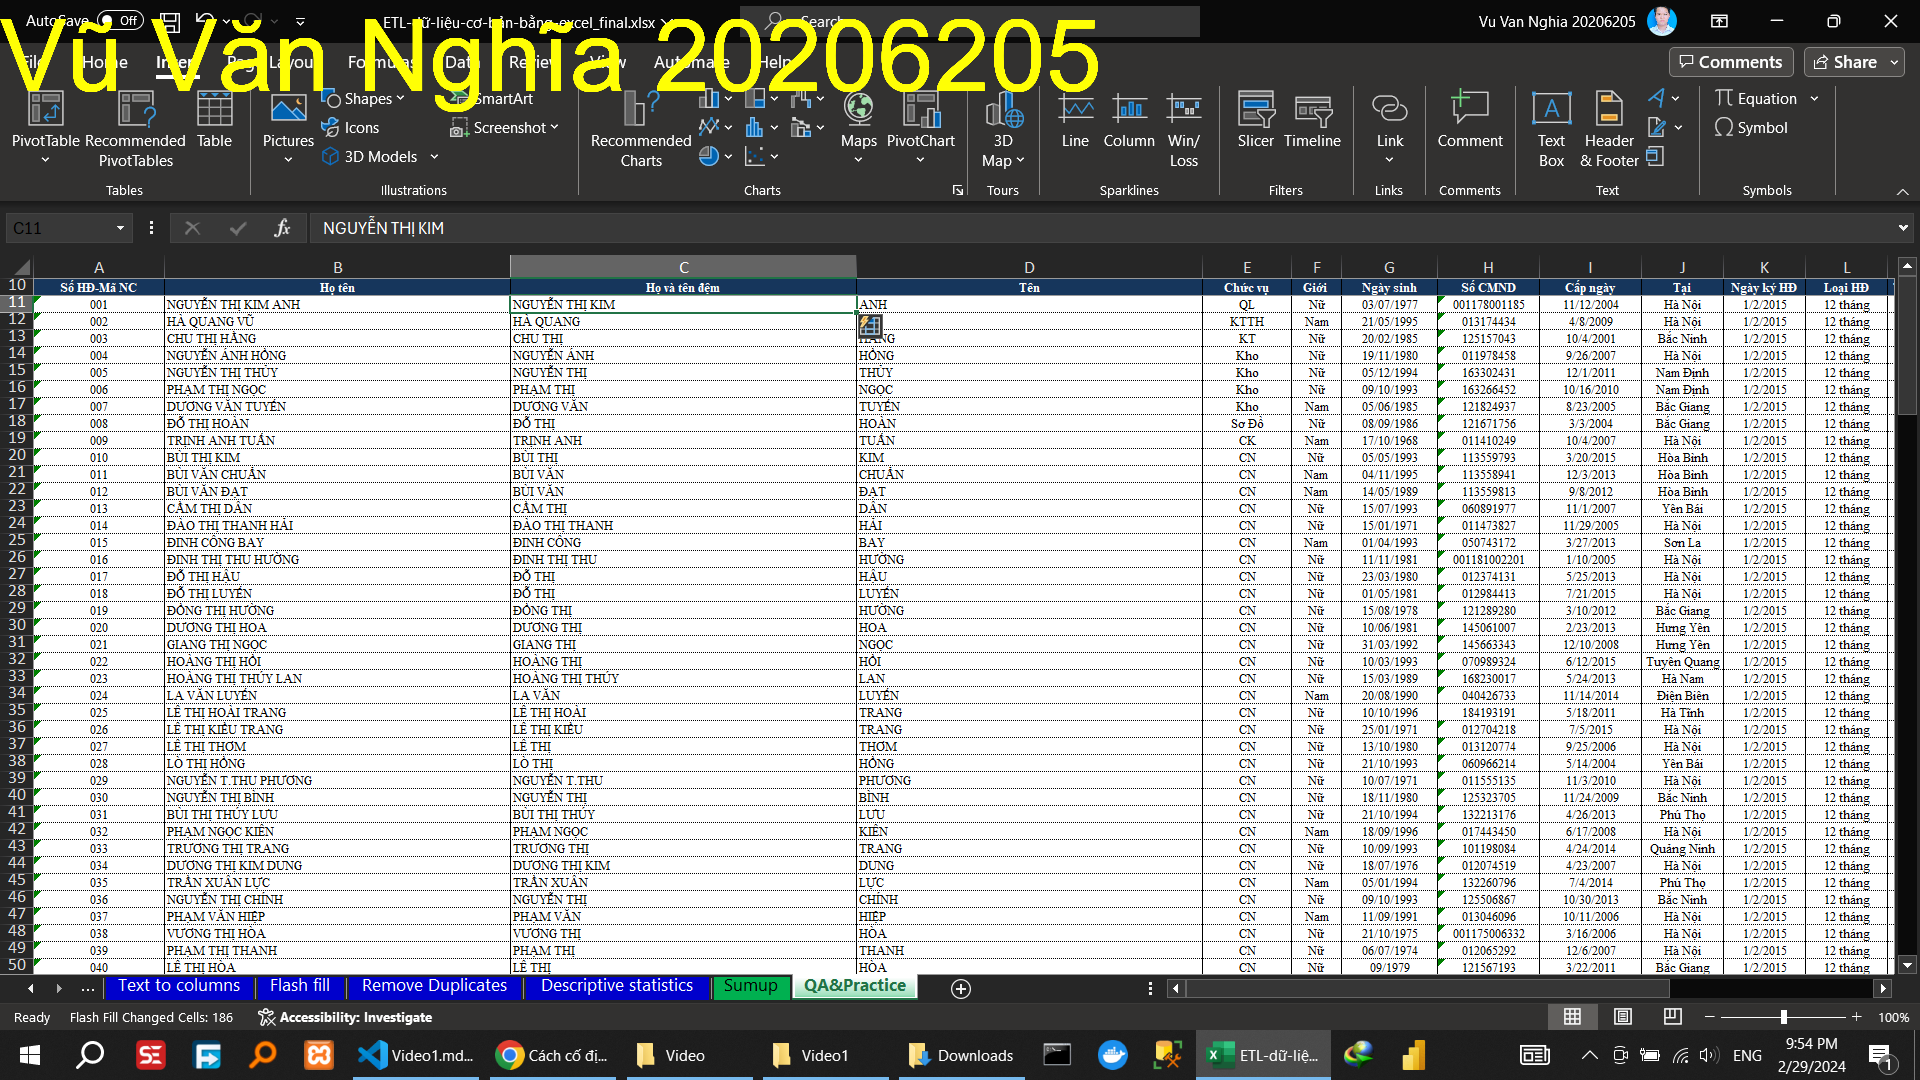
\includegraphics[scale = 0.15]{Video1/ThucHanh/4.png}
\caption{Thực hành tách họ và tên bằng flash fill}
\end{figure}

\begin{figure}[H]
\centering
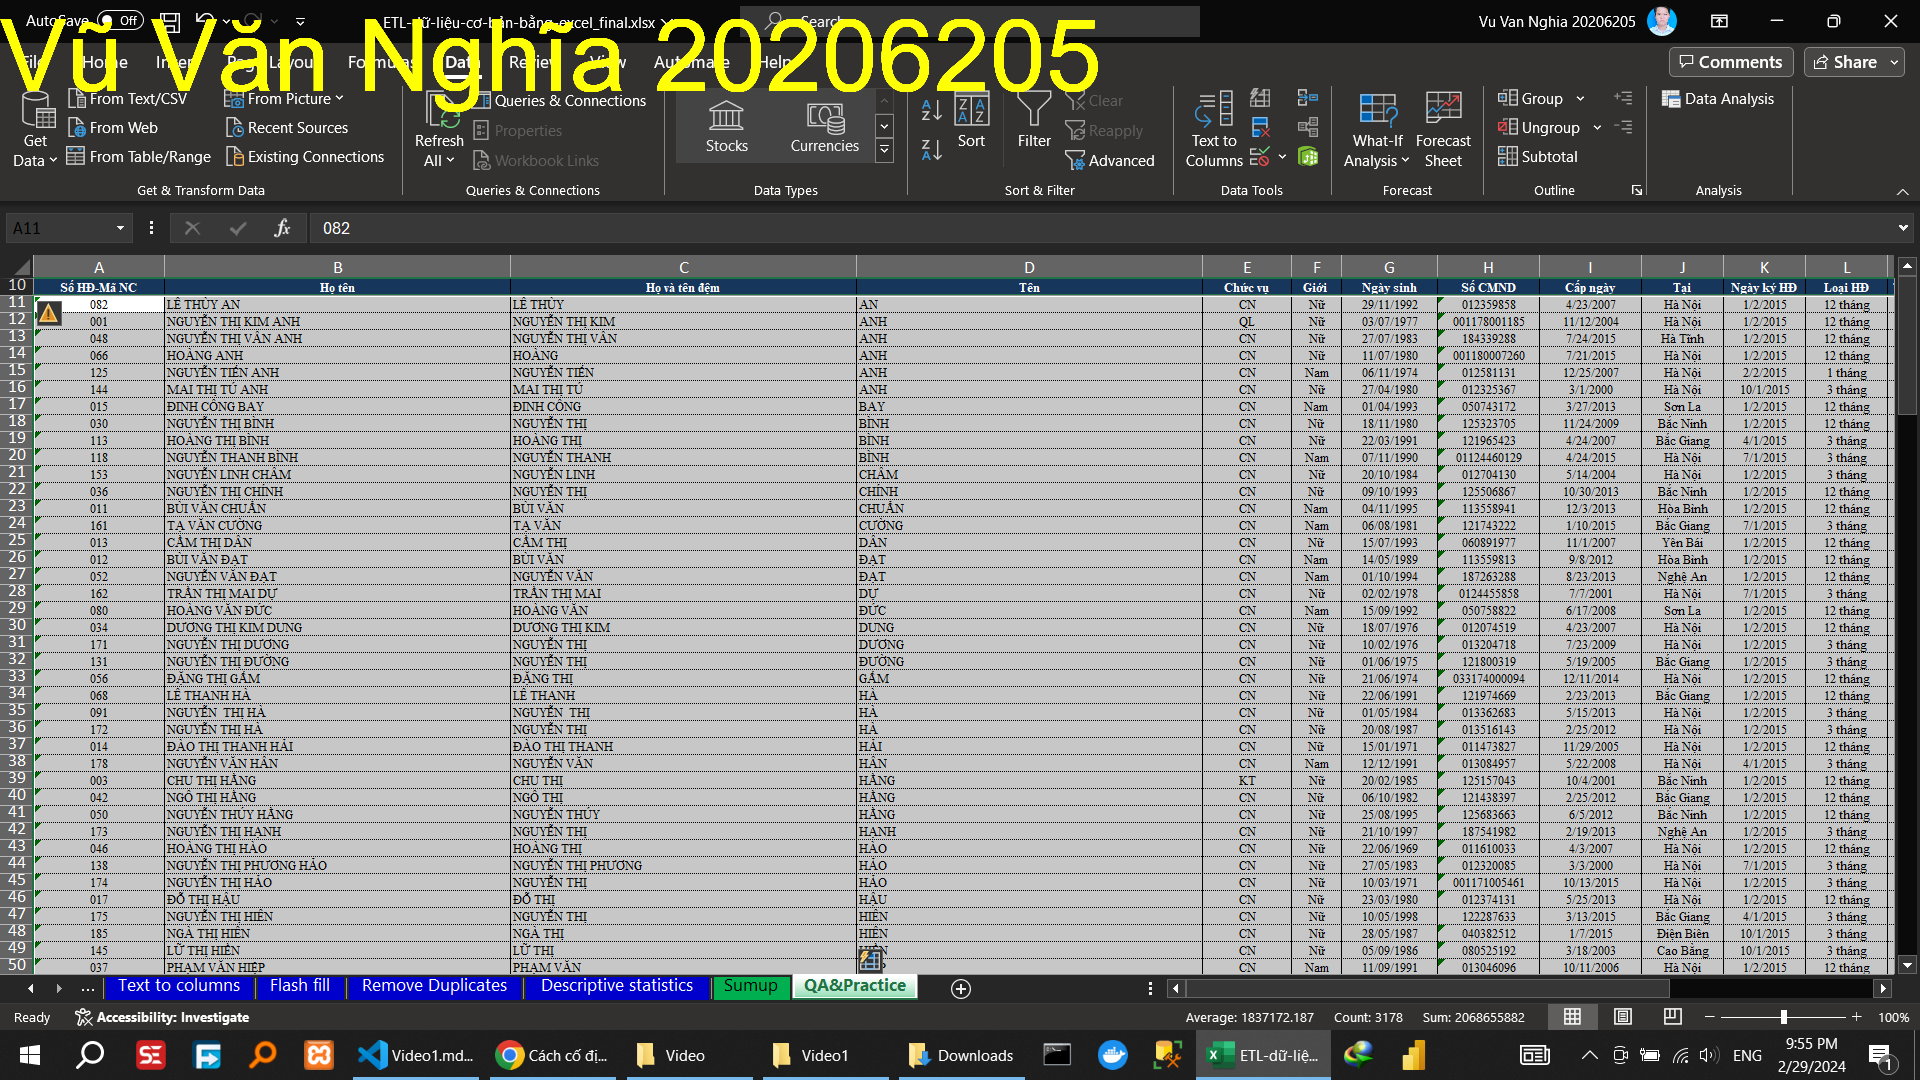
\includegraphics[scale = 0.15]{Video1/ThucHanh/5.png}
\caption{Thực hành sắp xếp danh sách theo tên nhân công}
\end{figure}

\begin{figure}[H]
\centering
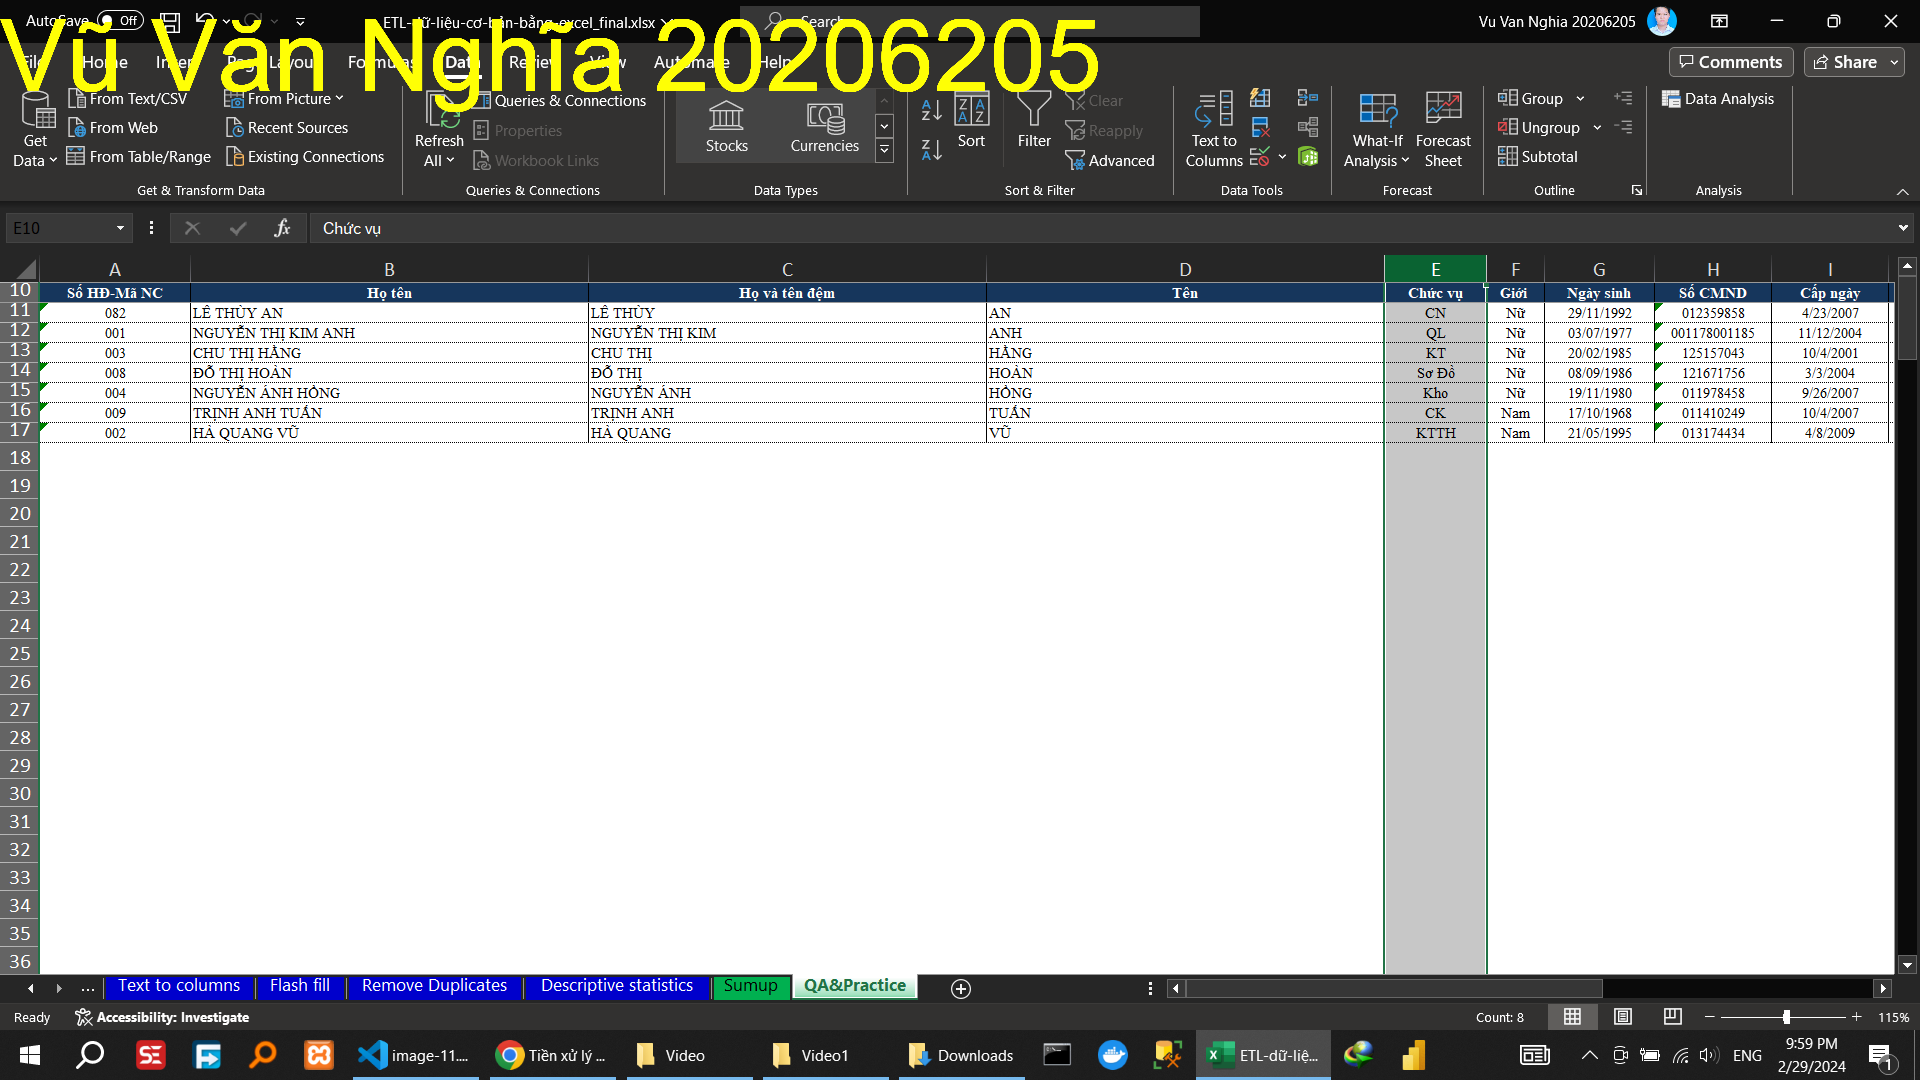
\includegraphics[scale = 0.15]{Video1/ThucHanh/6.png}
\caption{Thực hành lập danh sách các chức vụ của mỗi bộ phận}
\end{figure}
% %%%%%%%%%%%%%%%%%%%%%%%%%%%%%%%%%%%%%%%%%%%%%%%%%%%%%%%
\subsection{Video 2}
%%%%%%%%%%%%%%%%%%%%%%%%%%%%%%%%%%%%%%%%%%%%%%%%%%%%%%%
\begin{figure}[H]
\centering
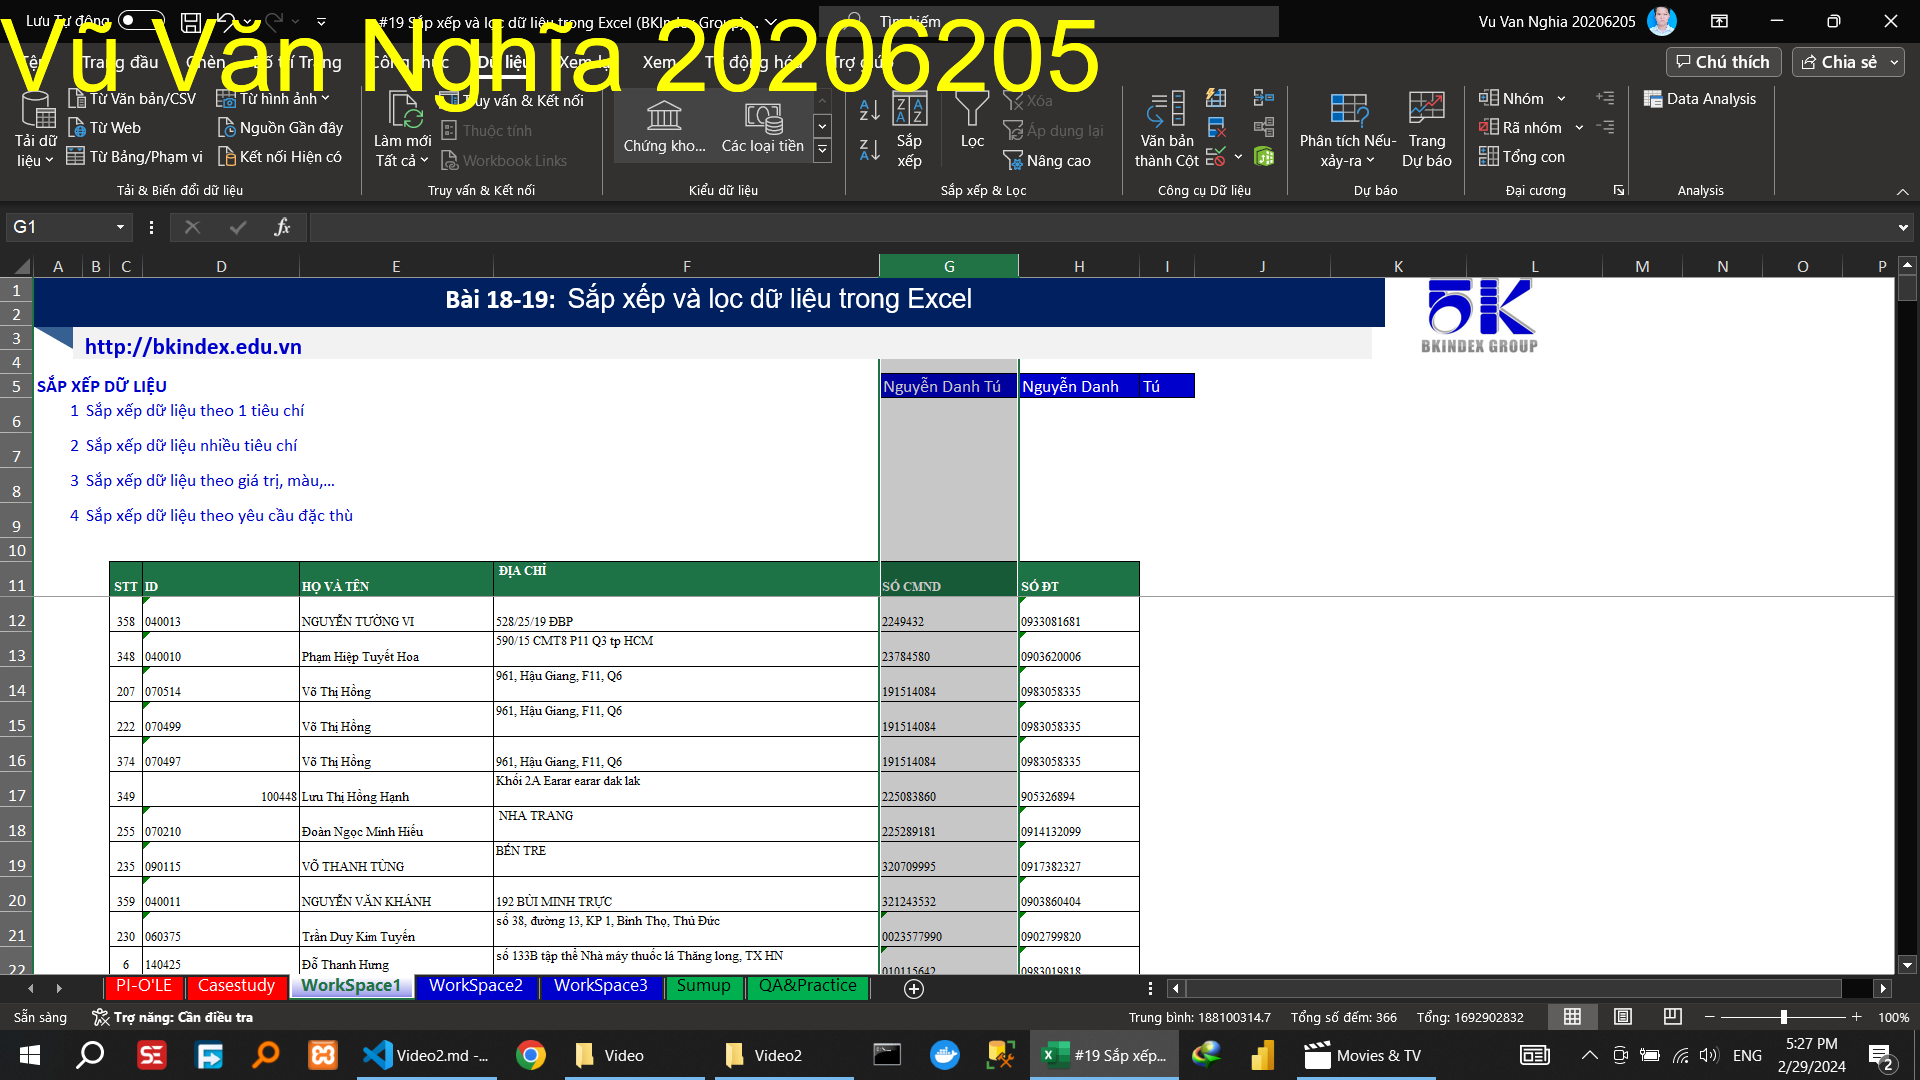
\includegraphics[scale = 0.15]{Video2/HuongDan/0.png}
\caption{Hướng dẫn sắp xếp dữ liệu theo 1 tiêu chí là số CMND}
\end{figure}

\begin{figure}[H]
\centering
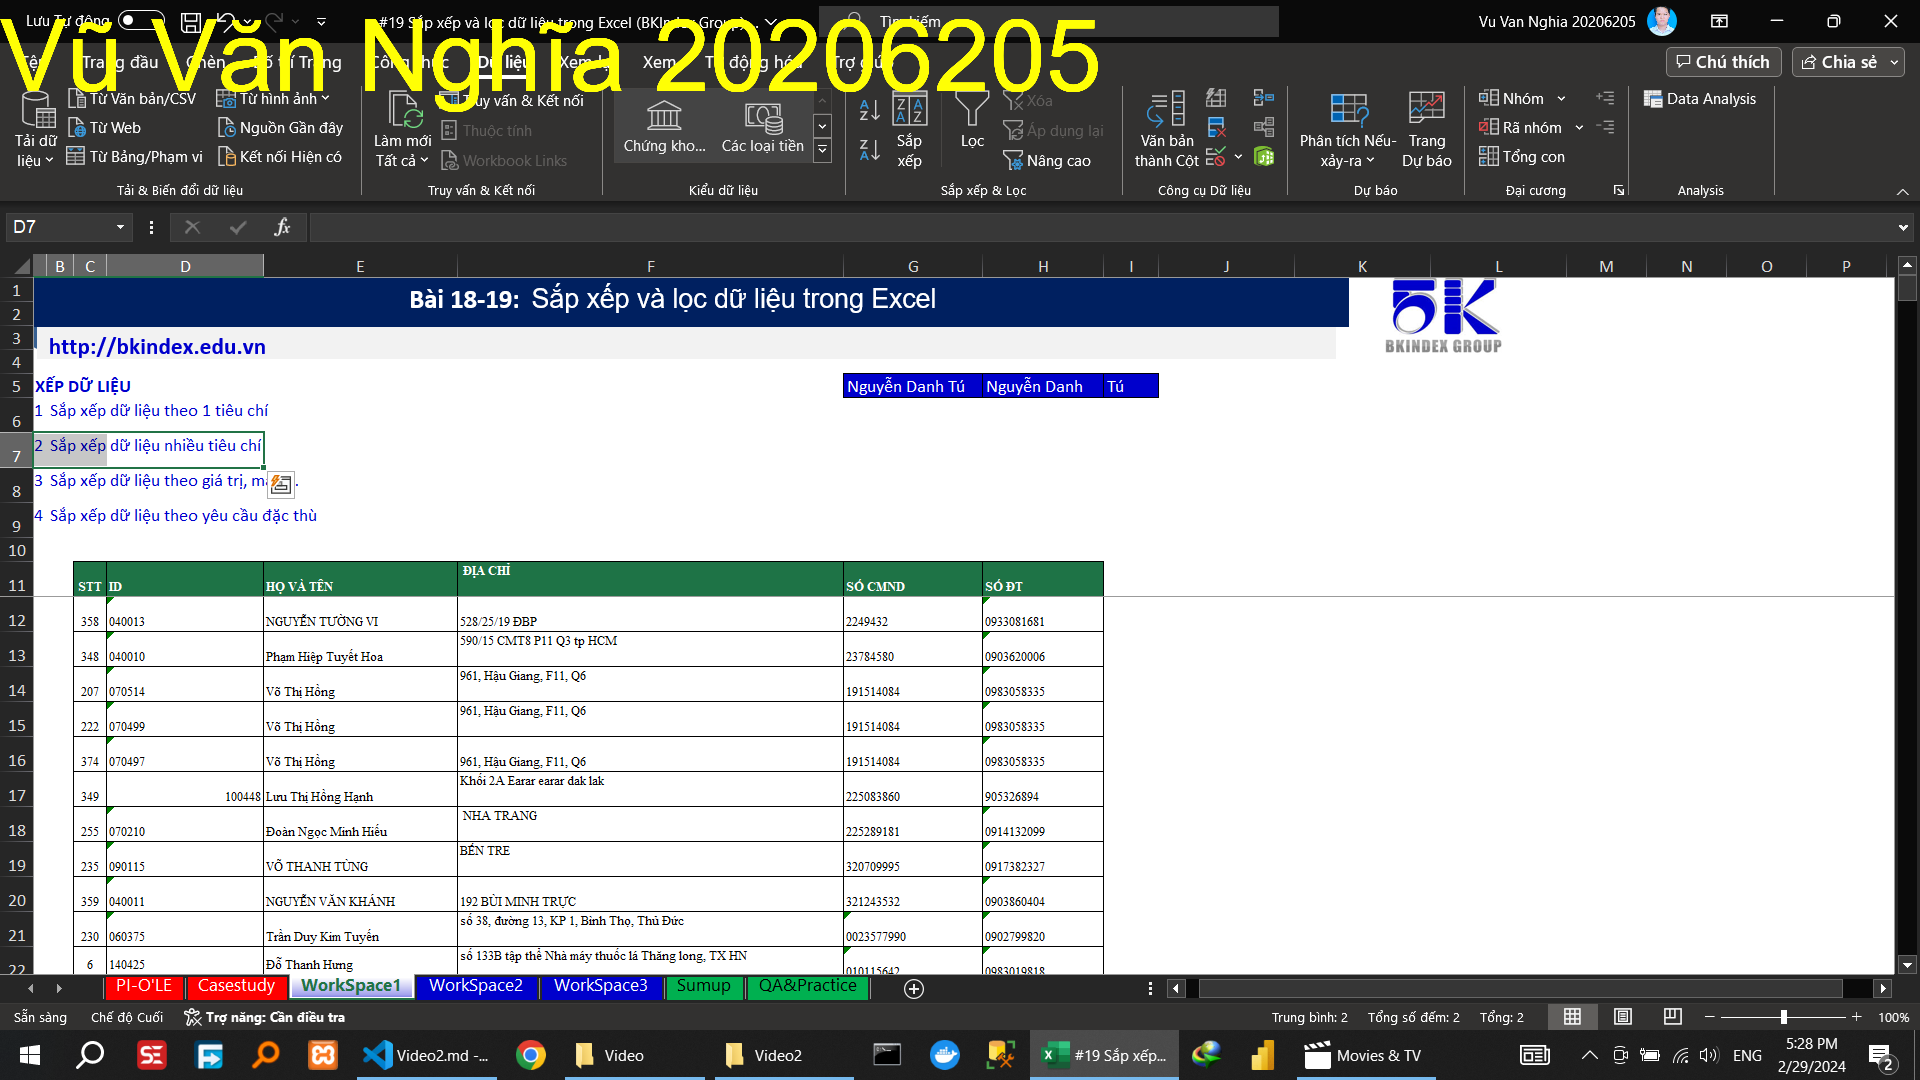
\includegraphics[scale = 0.15]{Video2/HuongDan/1.png}
\caption{Hướng dẫn sắp xếp dữ liệu theo nhiều tiêu chí số CMND và số điện thoại}
\end{figure}

\begin{figure}[H]
\centering
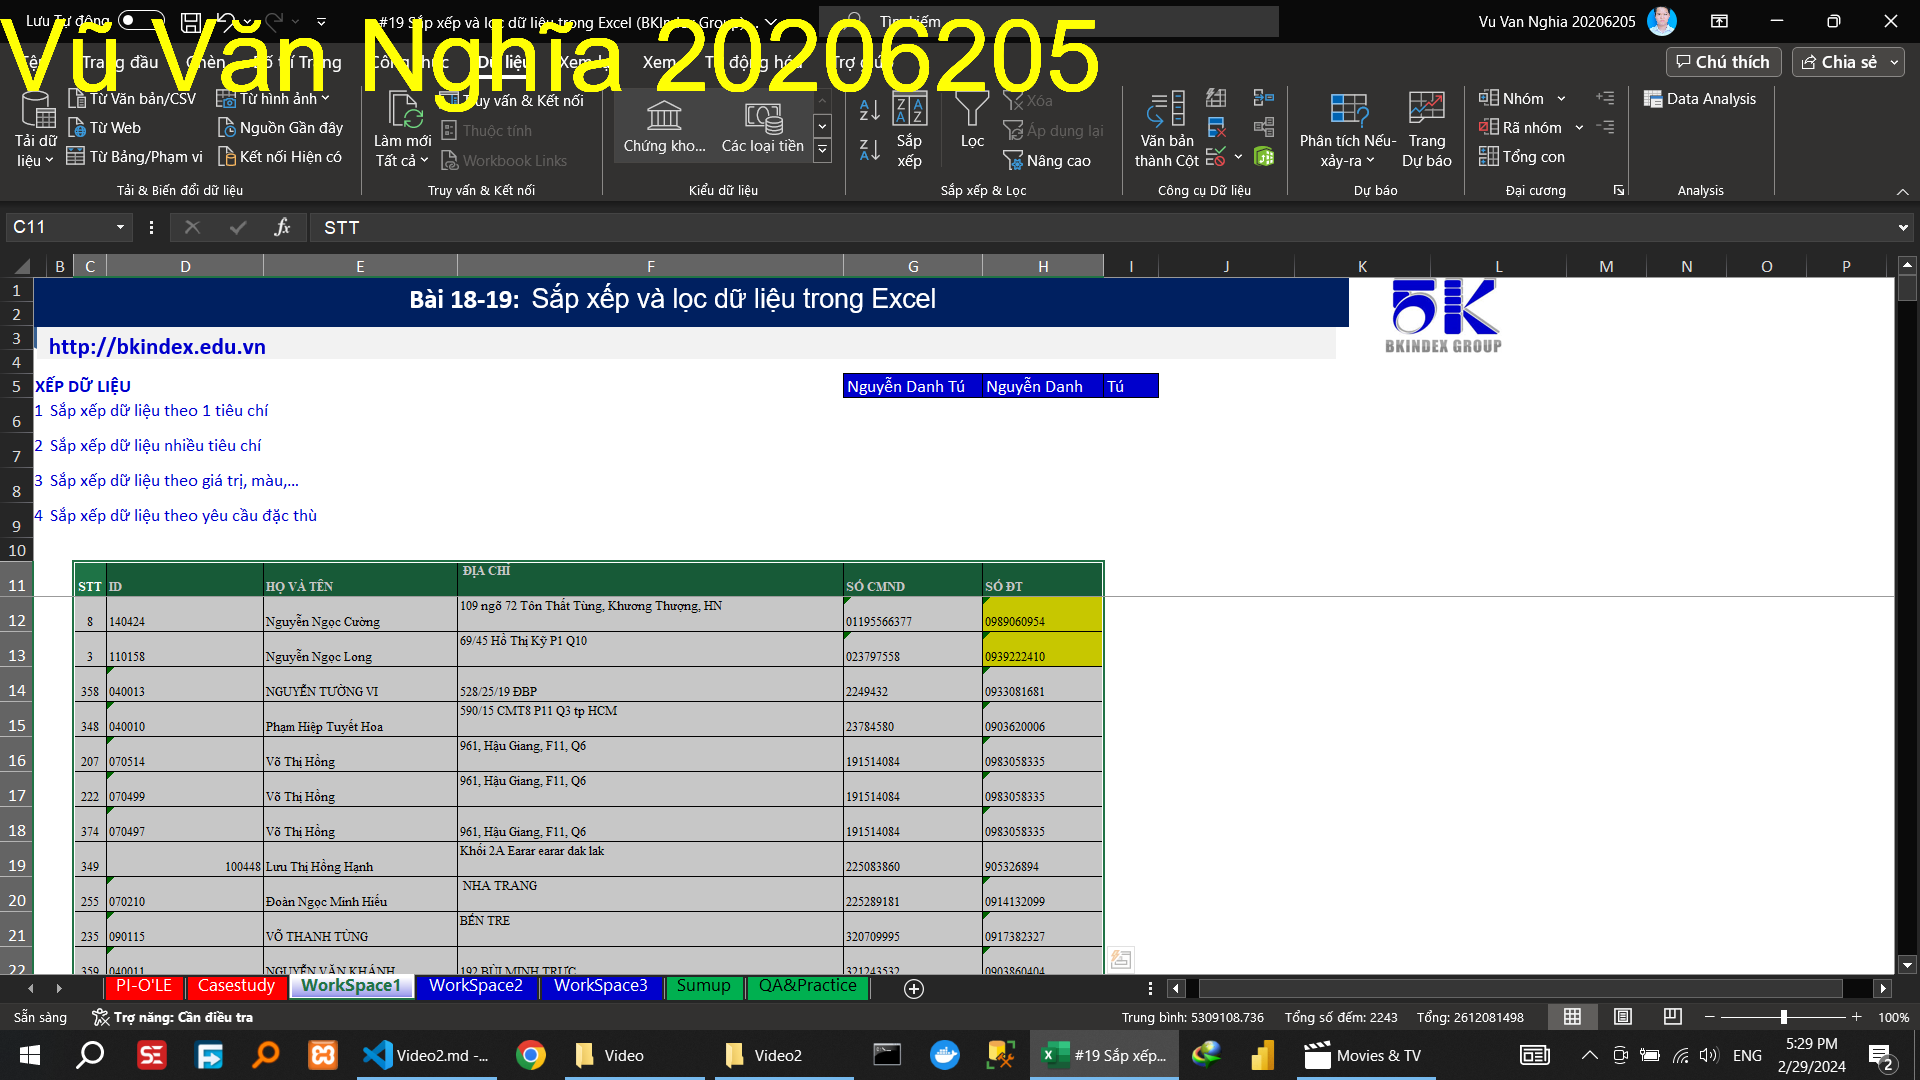
\includegraphics[scale = 0.15]{Video2/HuongDan/2.png}
\caption{Hướng dẫn sắp xếp dữ liệu theo giá trị, màu, \dots của số điện thoại}
\end{figure}

\begin{figure}[H]
\centering
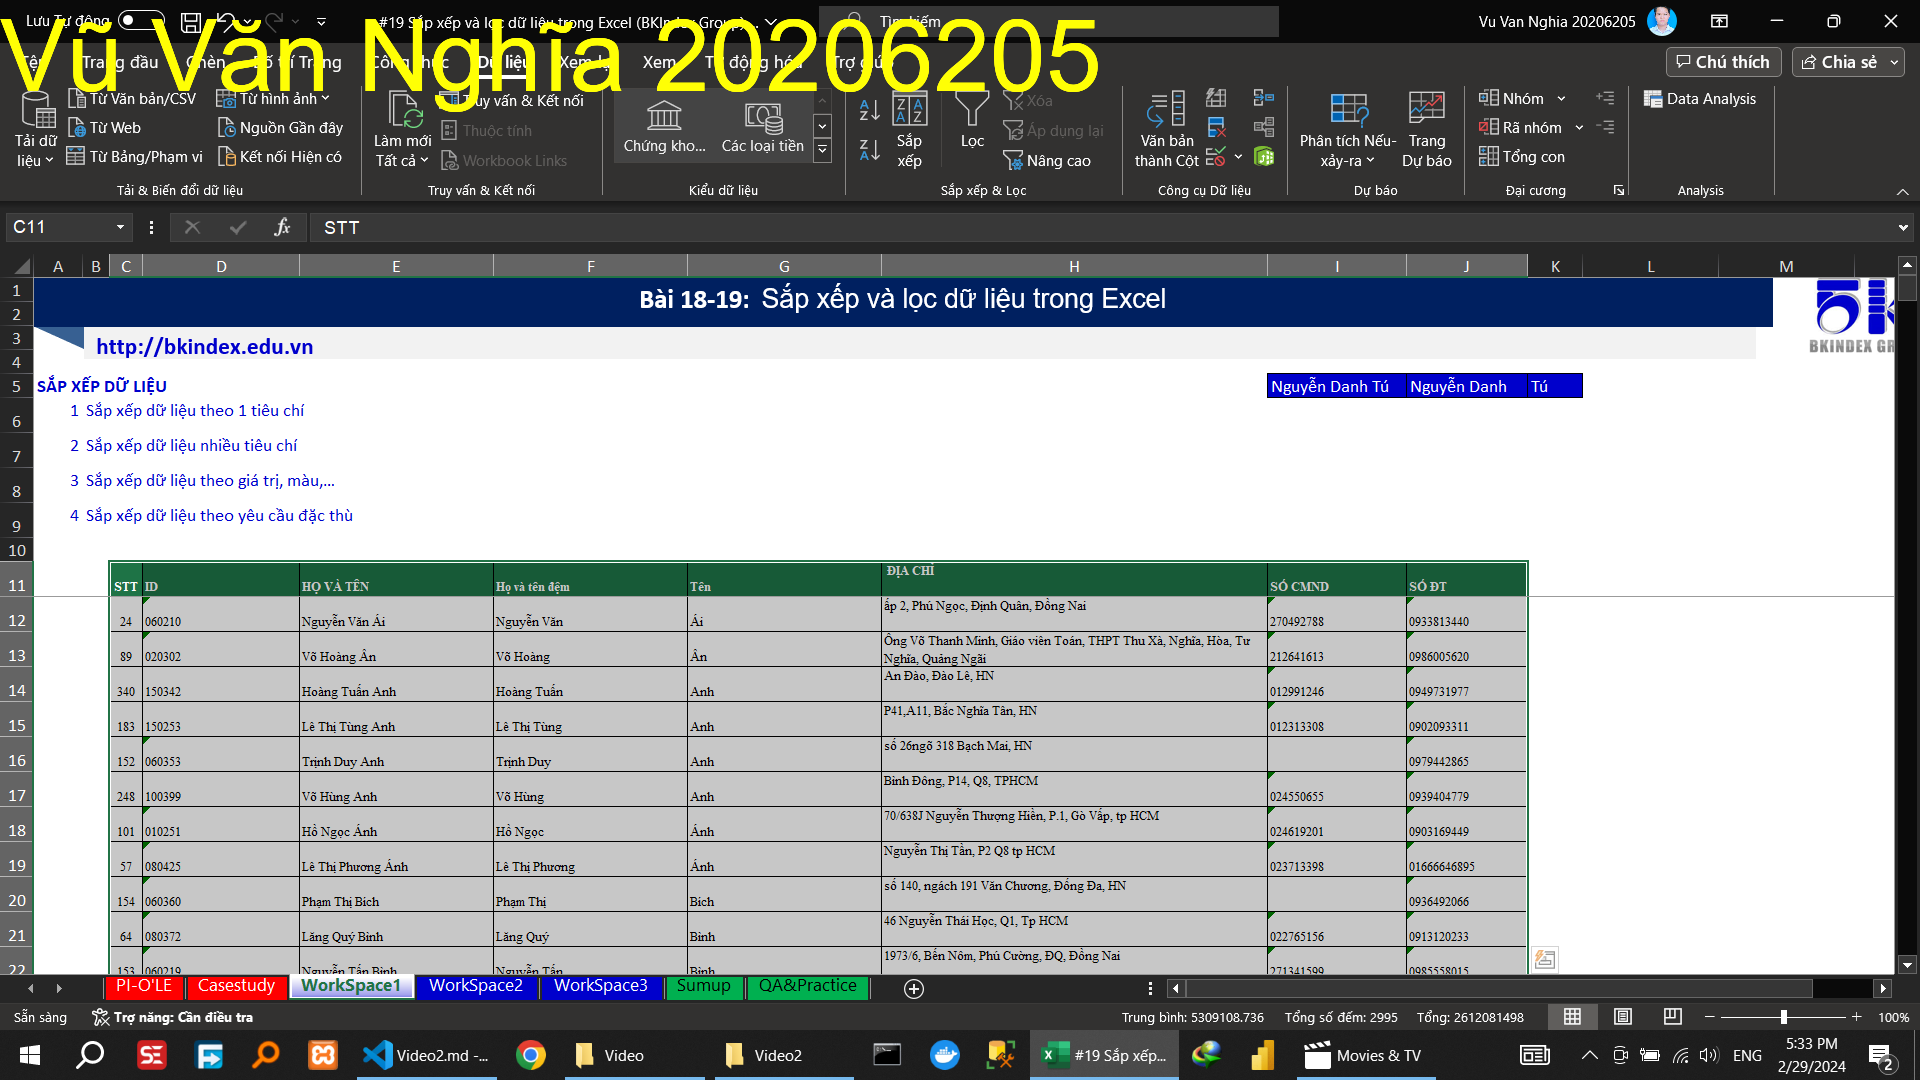
\includegraphics[scale = 0.15]{Video2/HuongDan/3.png}
\caption{Hướng dẫn sắp xếp dữ liệu theo yêu cầu đặc thù là tên và tên đệm}
\end{figure}

\begin{figure}[H]
\centering
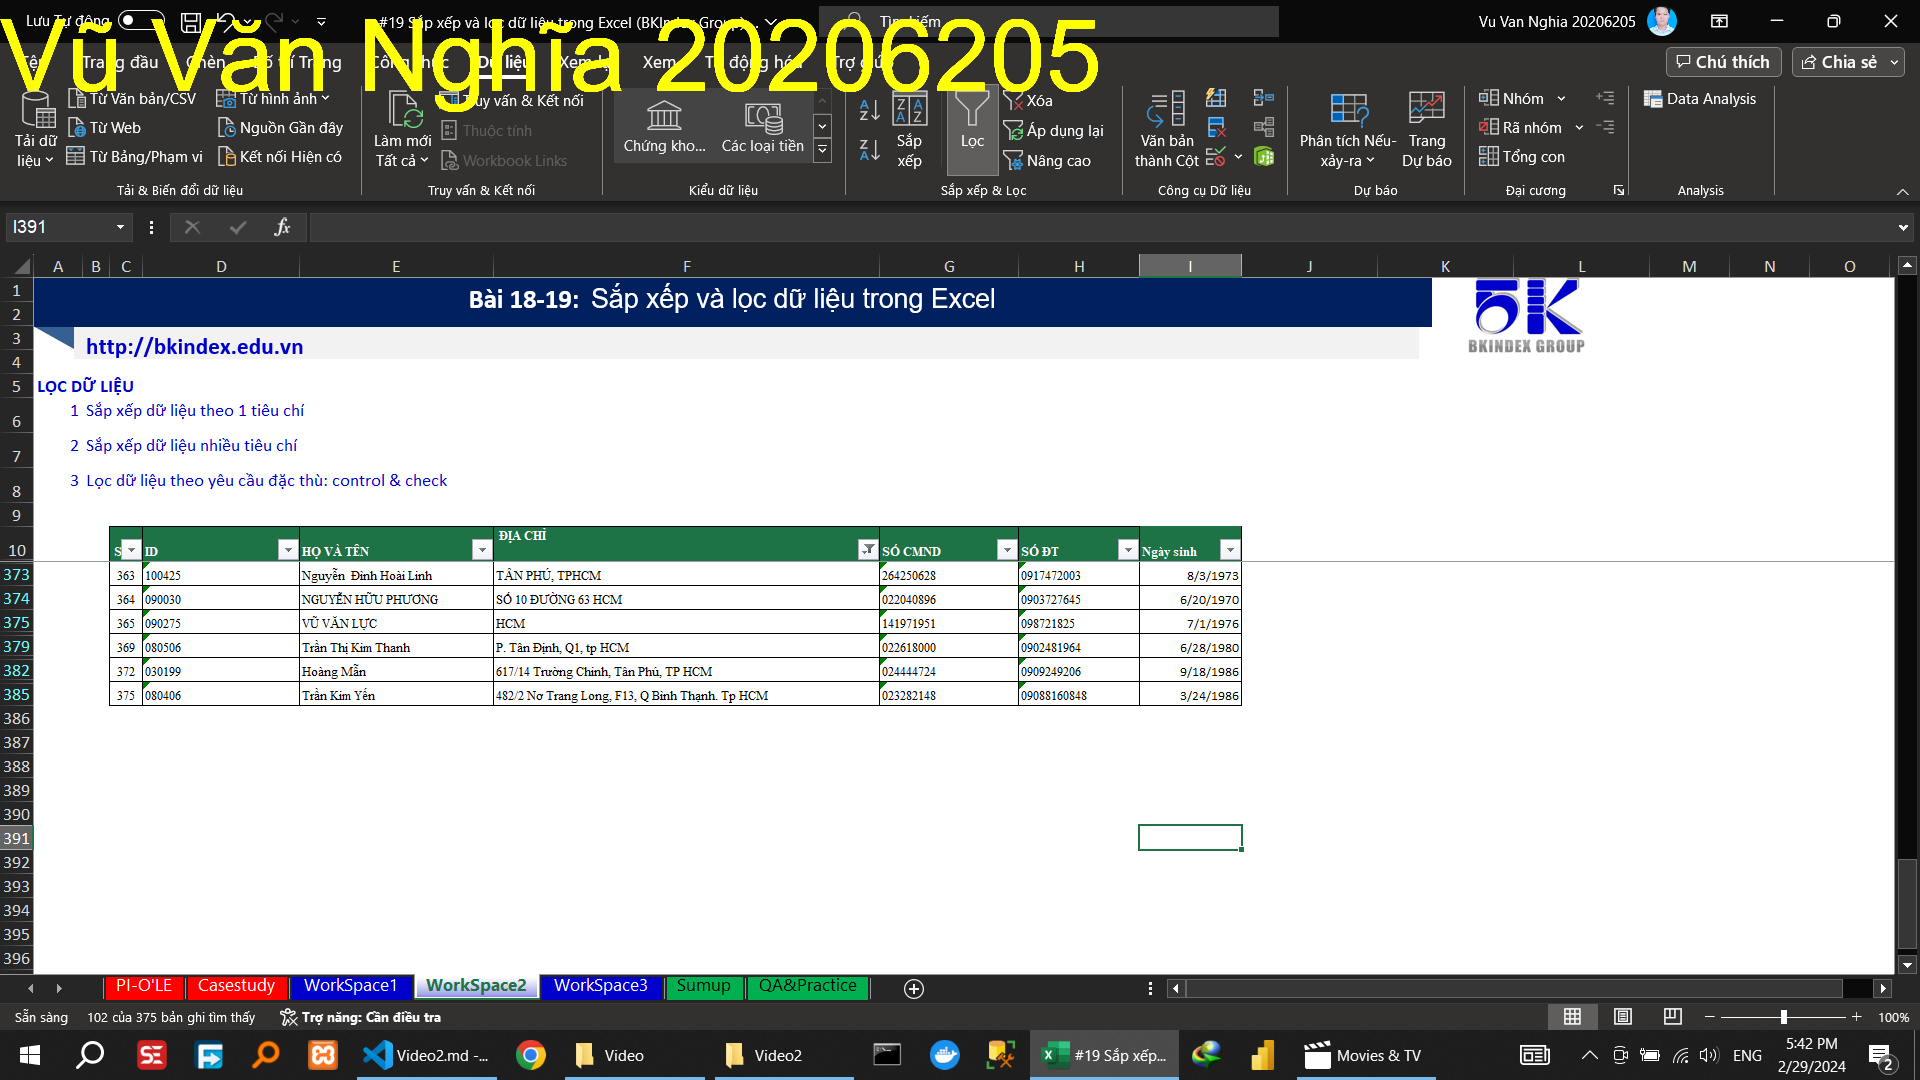
\includegraphics[scale = 0.15]{Video2/HuongDan/4.png}
\caption{Hướng dẫn lọc dữ liệu theo 1 tiêu chí là địa chỉ HCM}
\end{figure}

\begin{figure}[H]
\centering
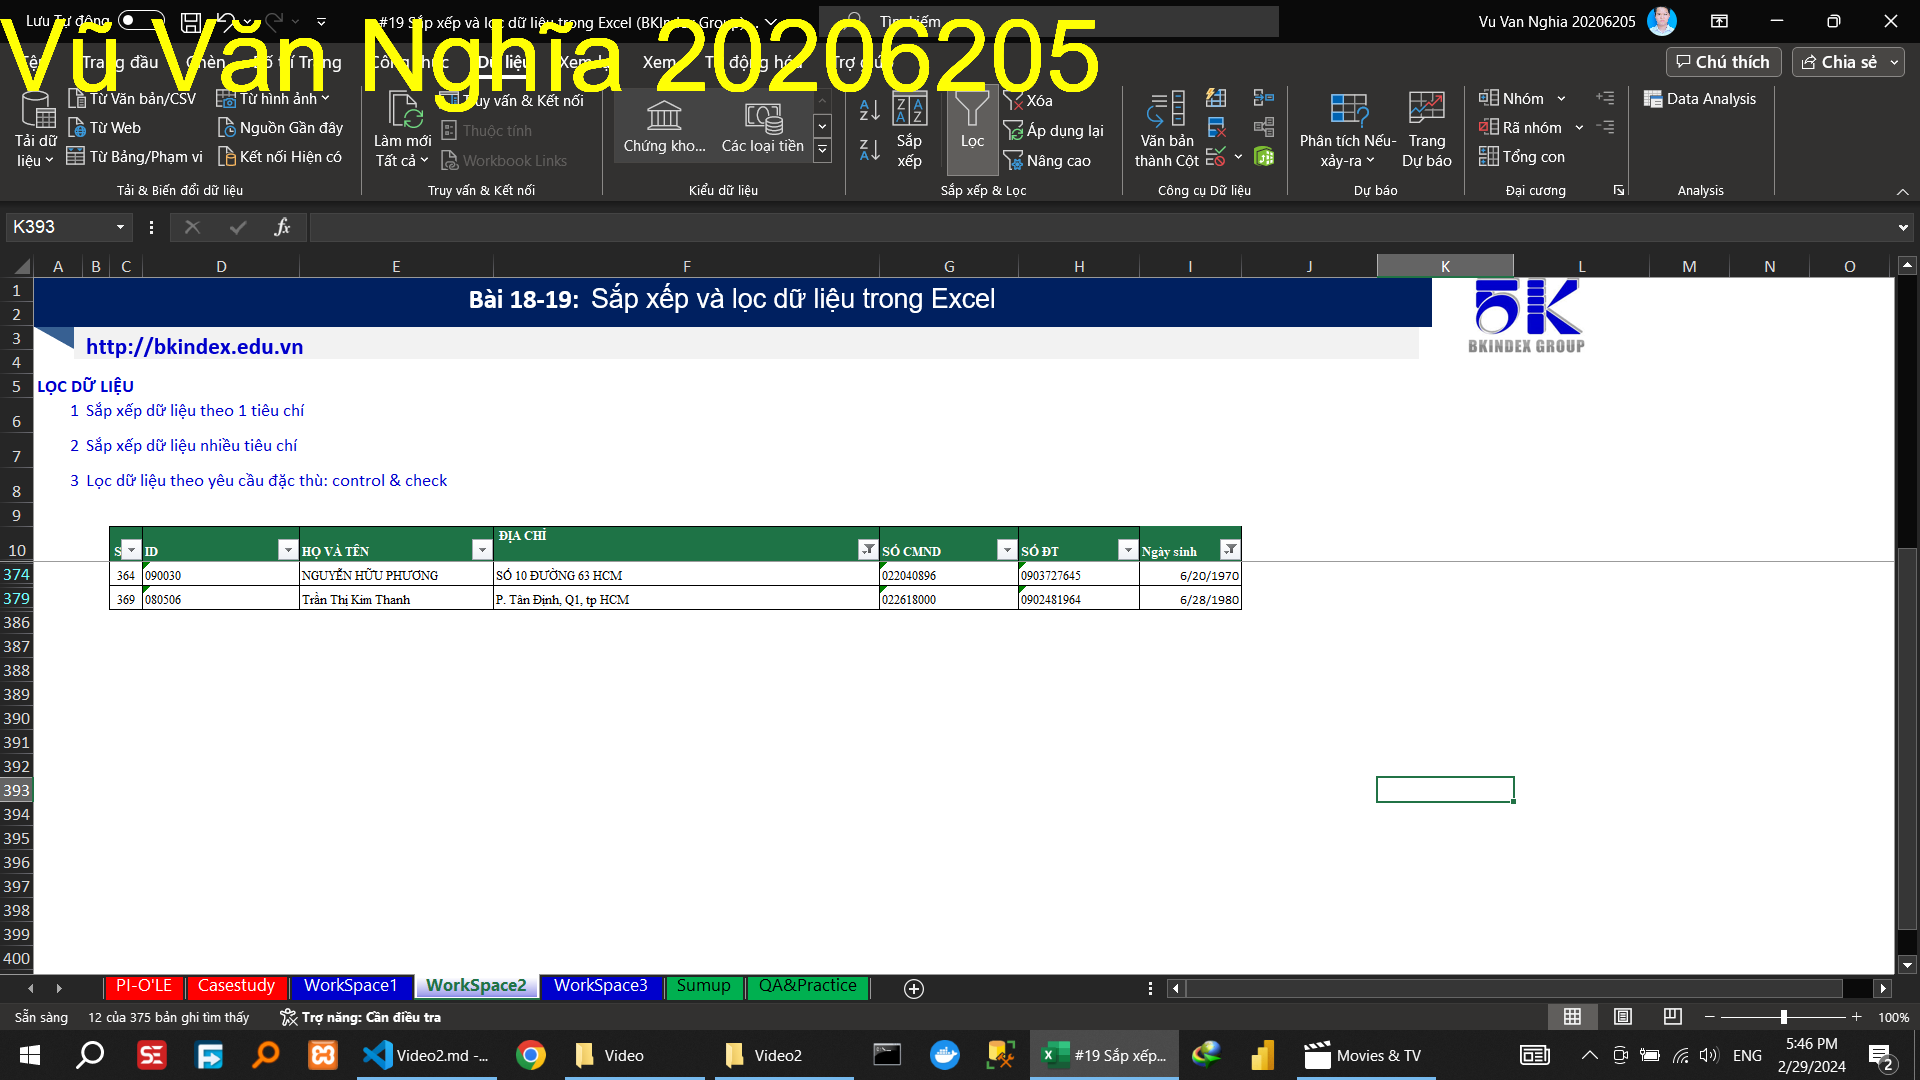
\includegraphics[scale = 0.15]{Video2/HuongDan/5.png}
\caption{Hướng dẫn lọc dữ liệu theo nhiều tiêu chí là sinh tháng 6 và ở HCM}
\end{figure}

\begin{figure}[H]
\centering
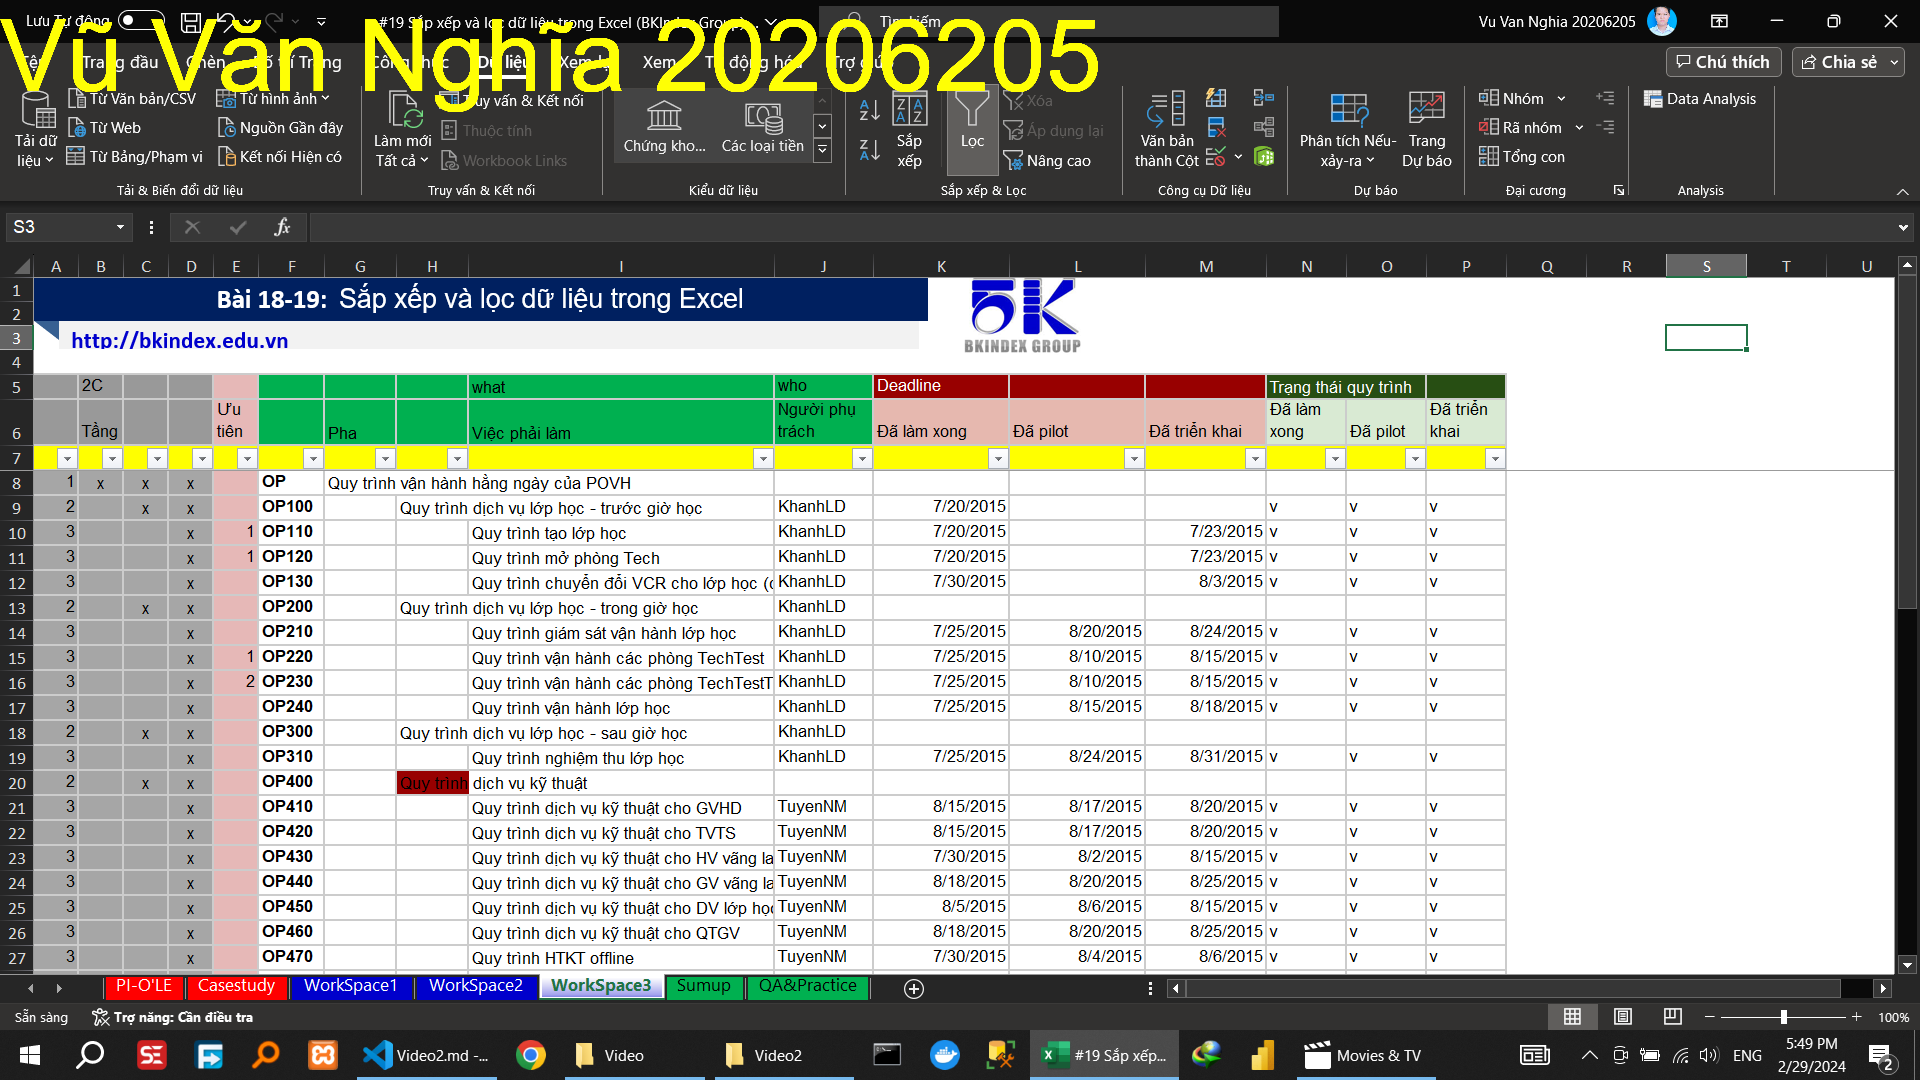
\includegraphics[scale = 0.15]{Video2/HuongDan/6.png}
\caption{Hướng dẫn lọc dữ liệu theo yêu cầu đặc thù: control và check}
\end{figure}
% %%%%%%%%%%%%%%%%%%%%%%%%%%%%%%%%%%%%%%%%%%%%%%%%%%%%%%%
\begin{figure}[H]
\centering
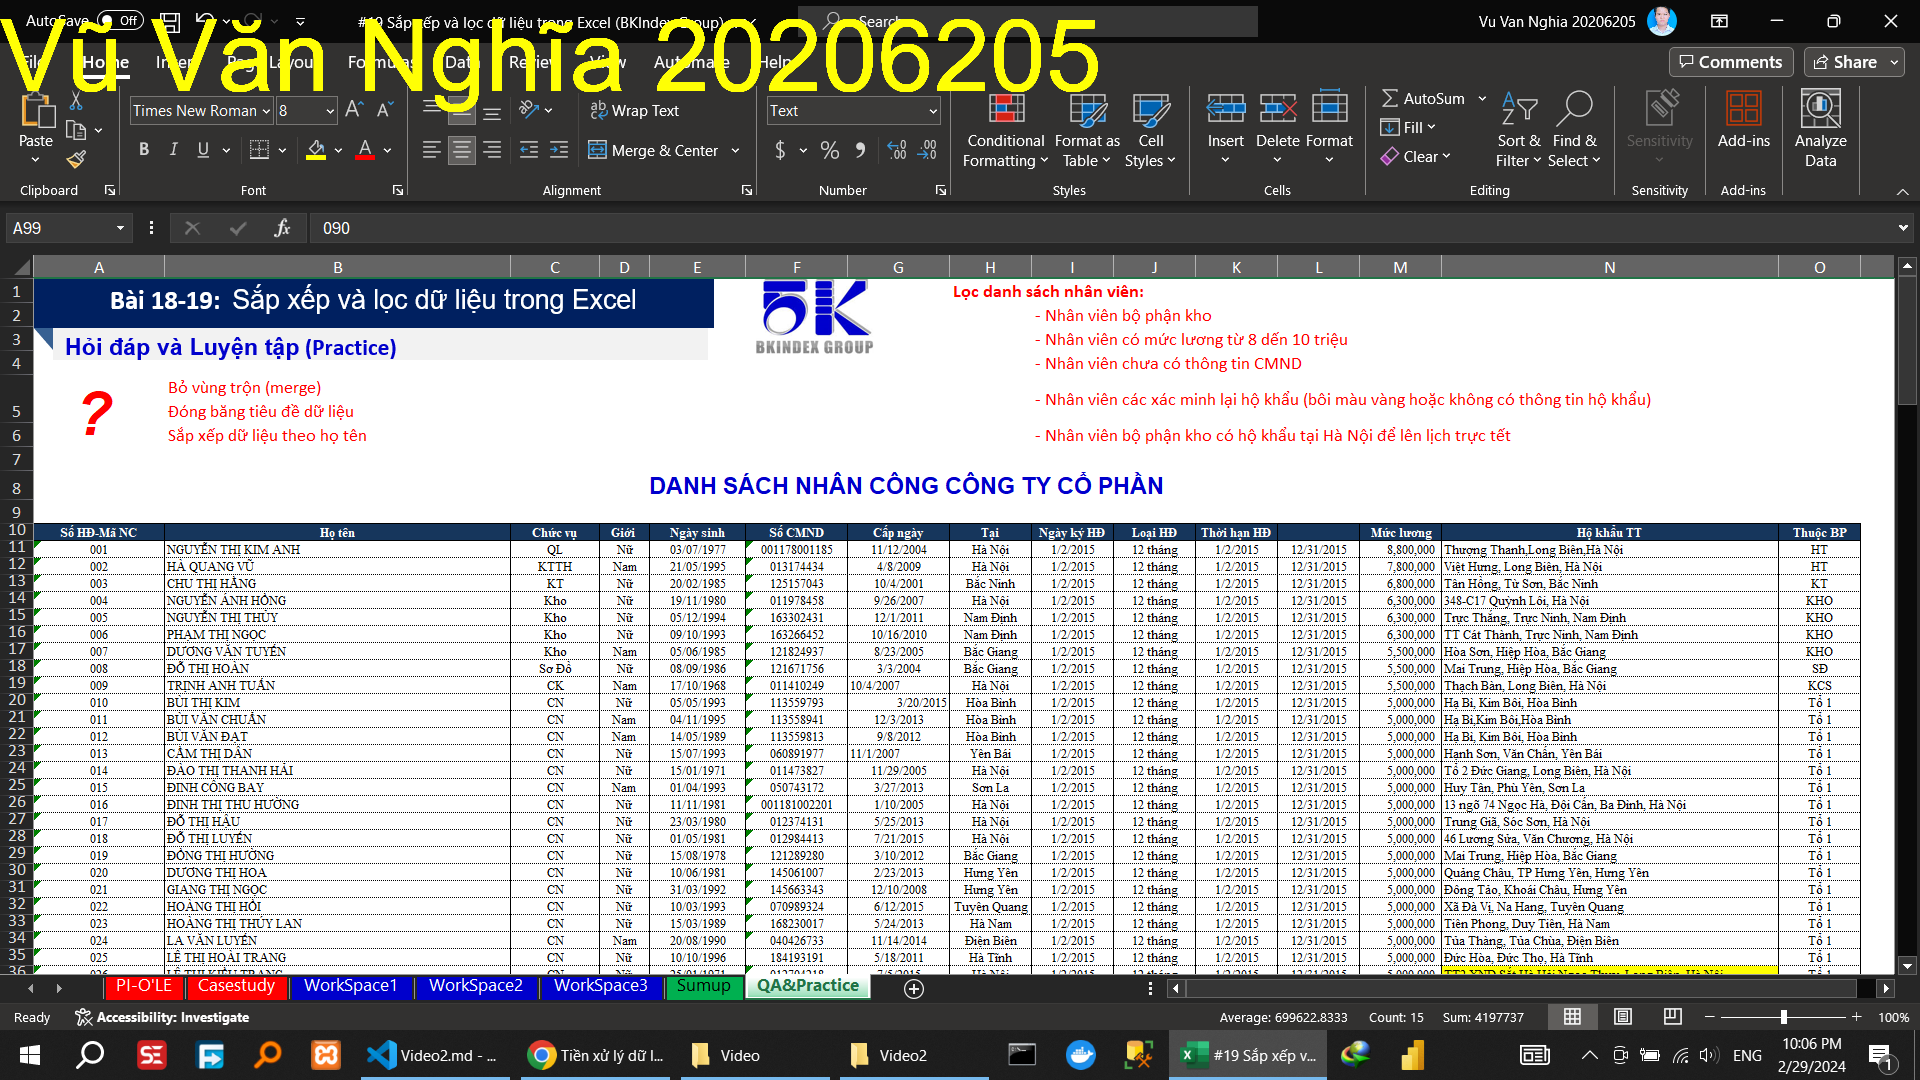
\includegraphics[scale = 0.15]{Video2/ThucHanh/0.png}
\caption{Thực hành bỏ vùng trộn (merge)}
\end{figure}

\begin{figure}[H]
\centering
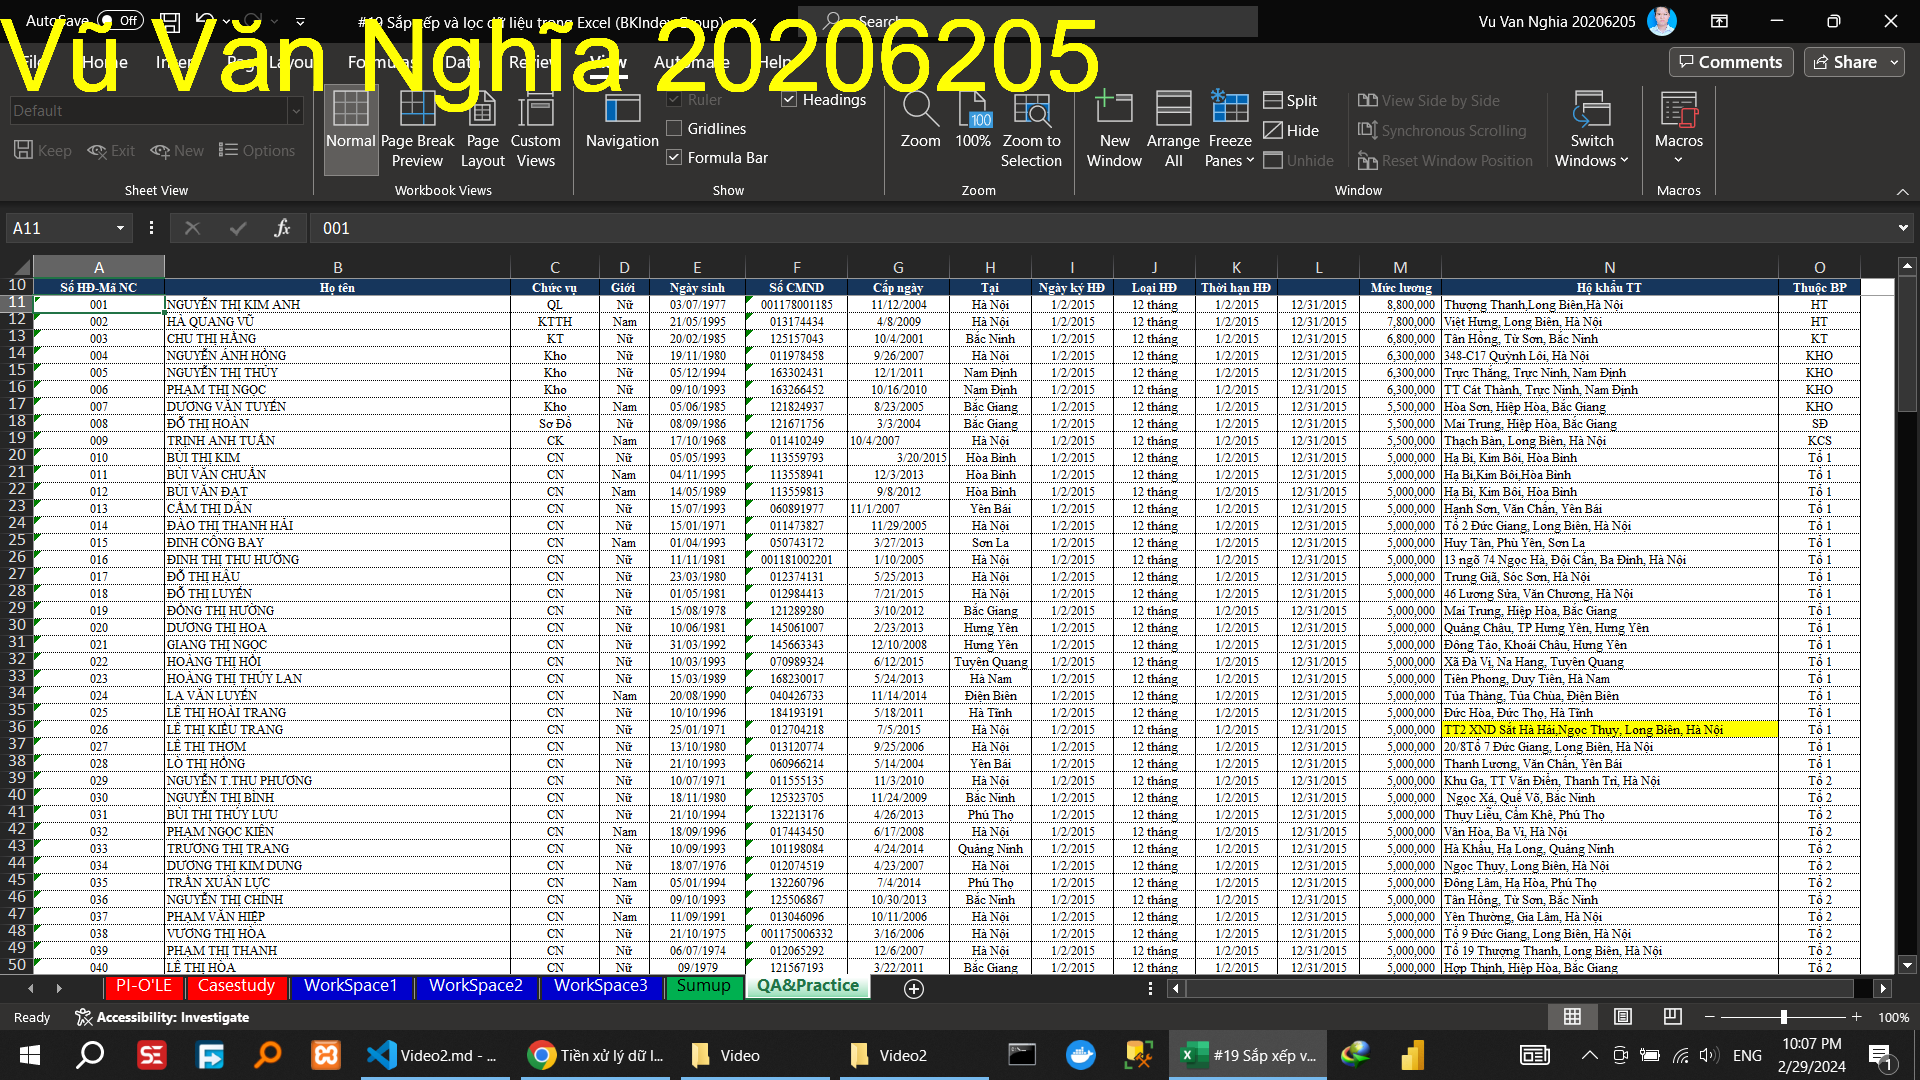
\includegraphics[scale = 0.15]{Video2/ThucHanh/1.png}
\caption{Thực hành đóng băng tiêu đề dữ liệu}
\end{figure}

\begin{figure}[H]
\centering
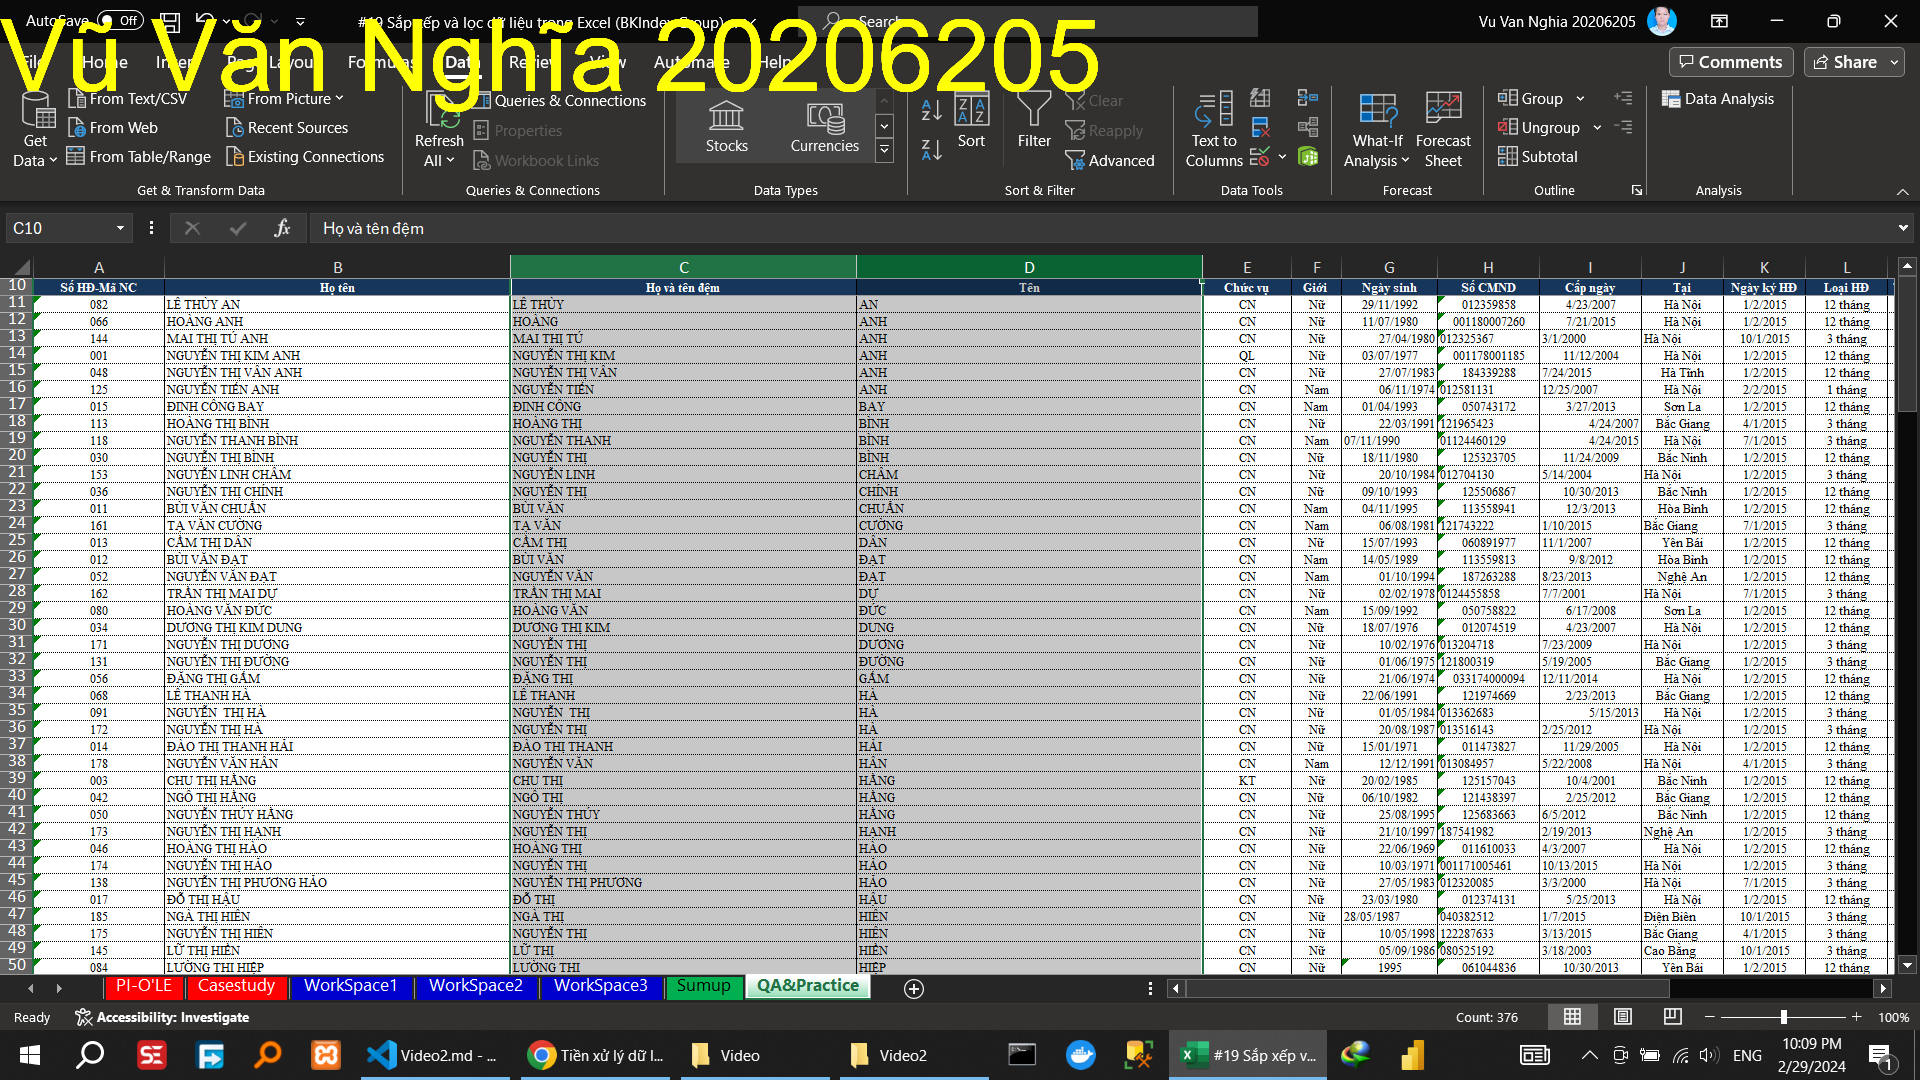
\includegraphics[scale = 0.15]{Video2/ThucHanh/2.png}
\caption{Thực hành sắp xếp dữ liệu theo họ tên}
\end{figure}

\begin{figure}[H]
\centering
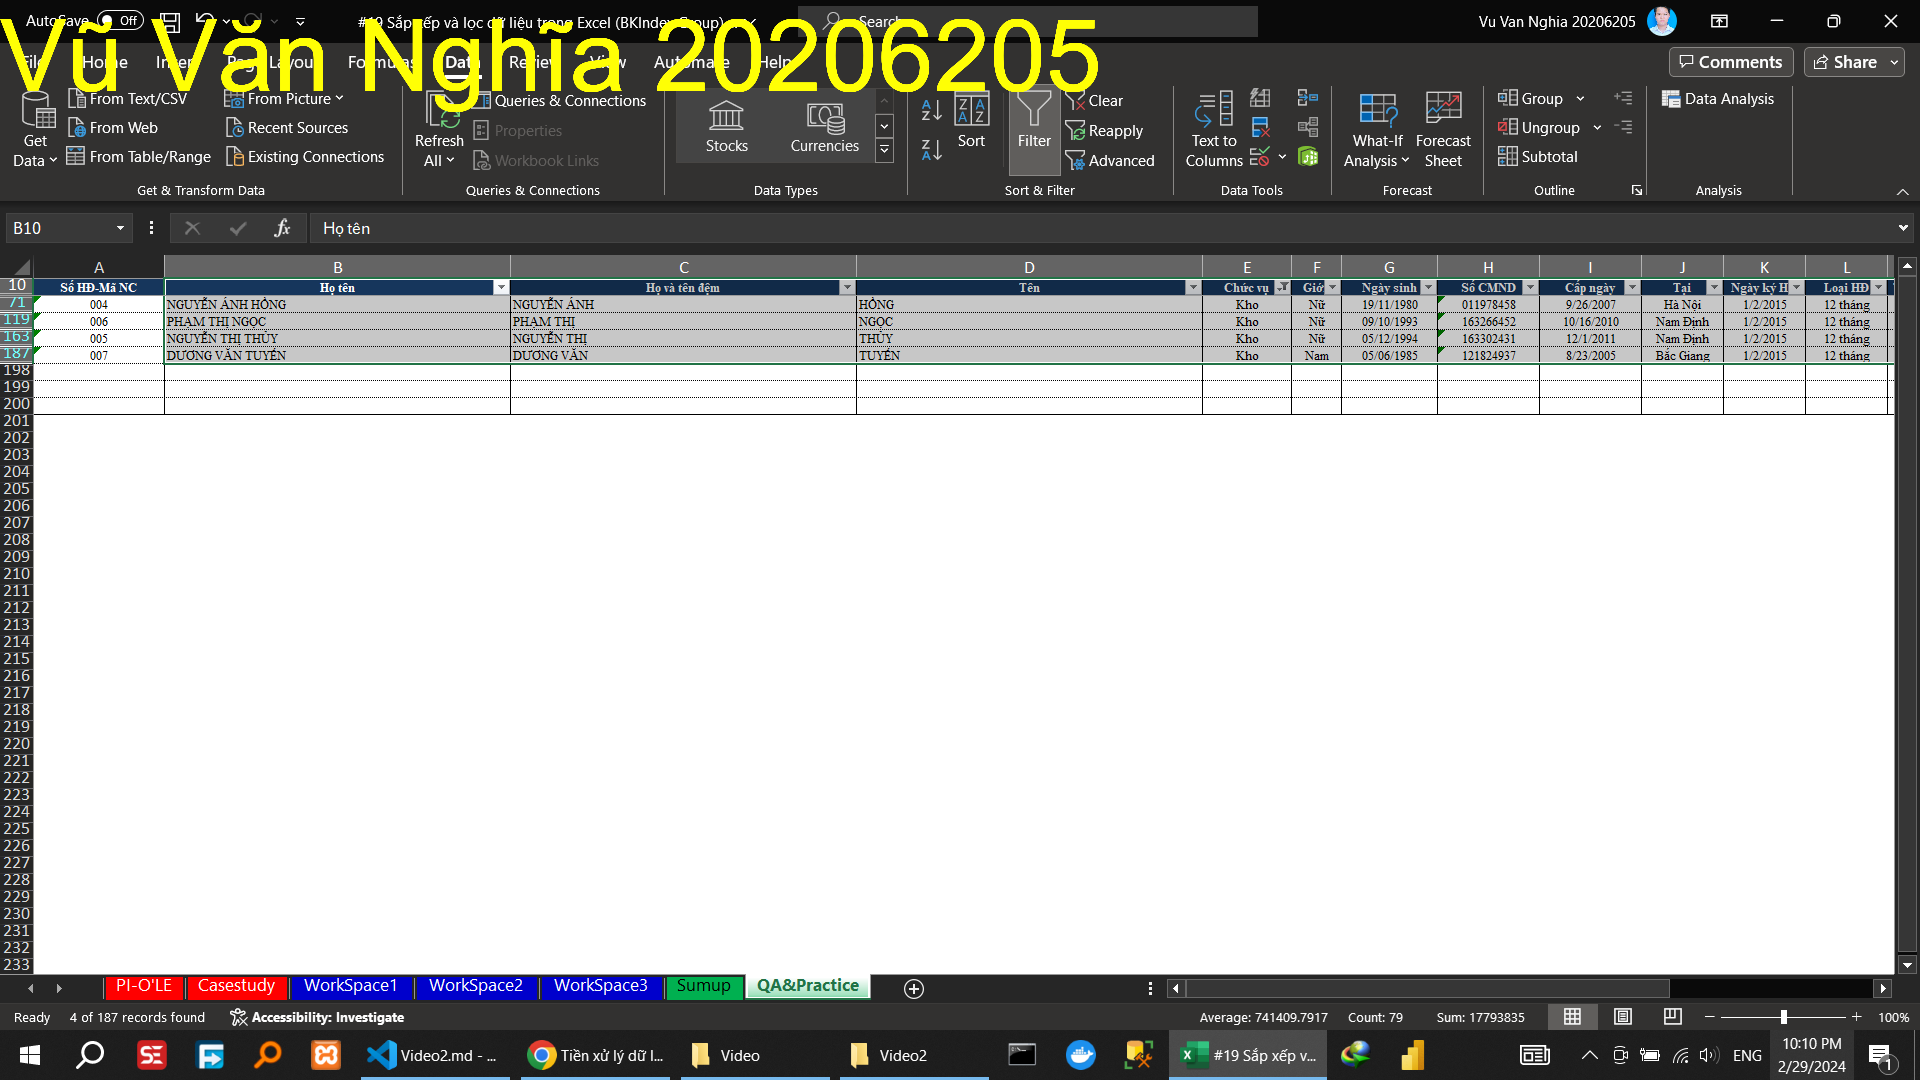
\includegraphics[scale = 0.15]{Video2/ThucHanh/3.png}
\caption{Thực hành lọc danh sách nhân viên bộ phận kho}
\end{figure}

\begin{figure}[H]
\centering
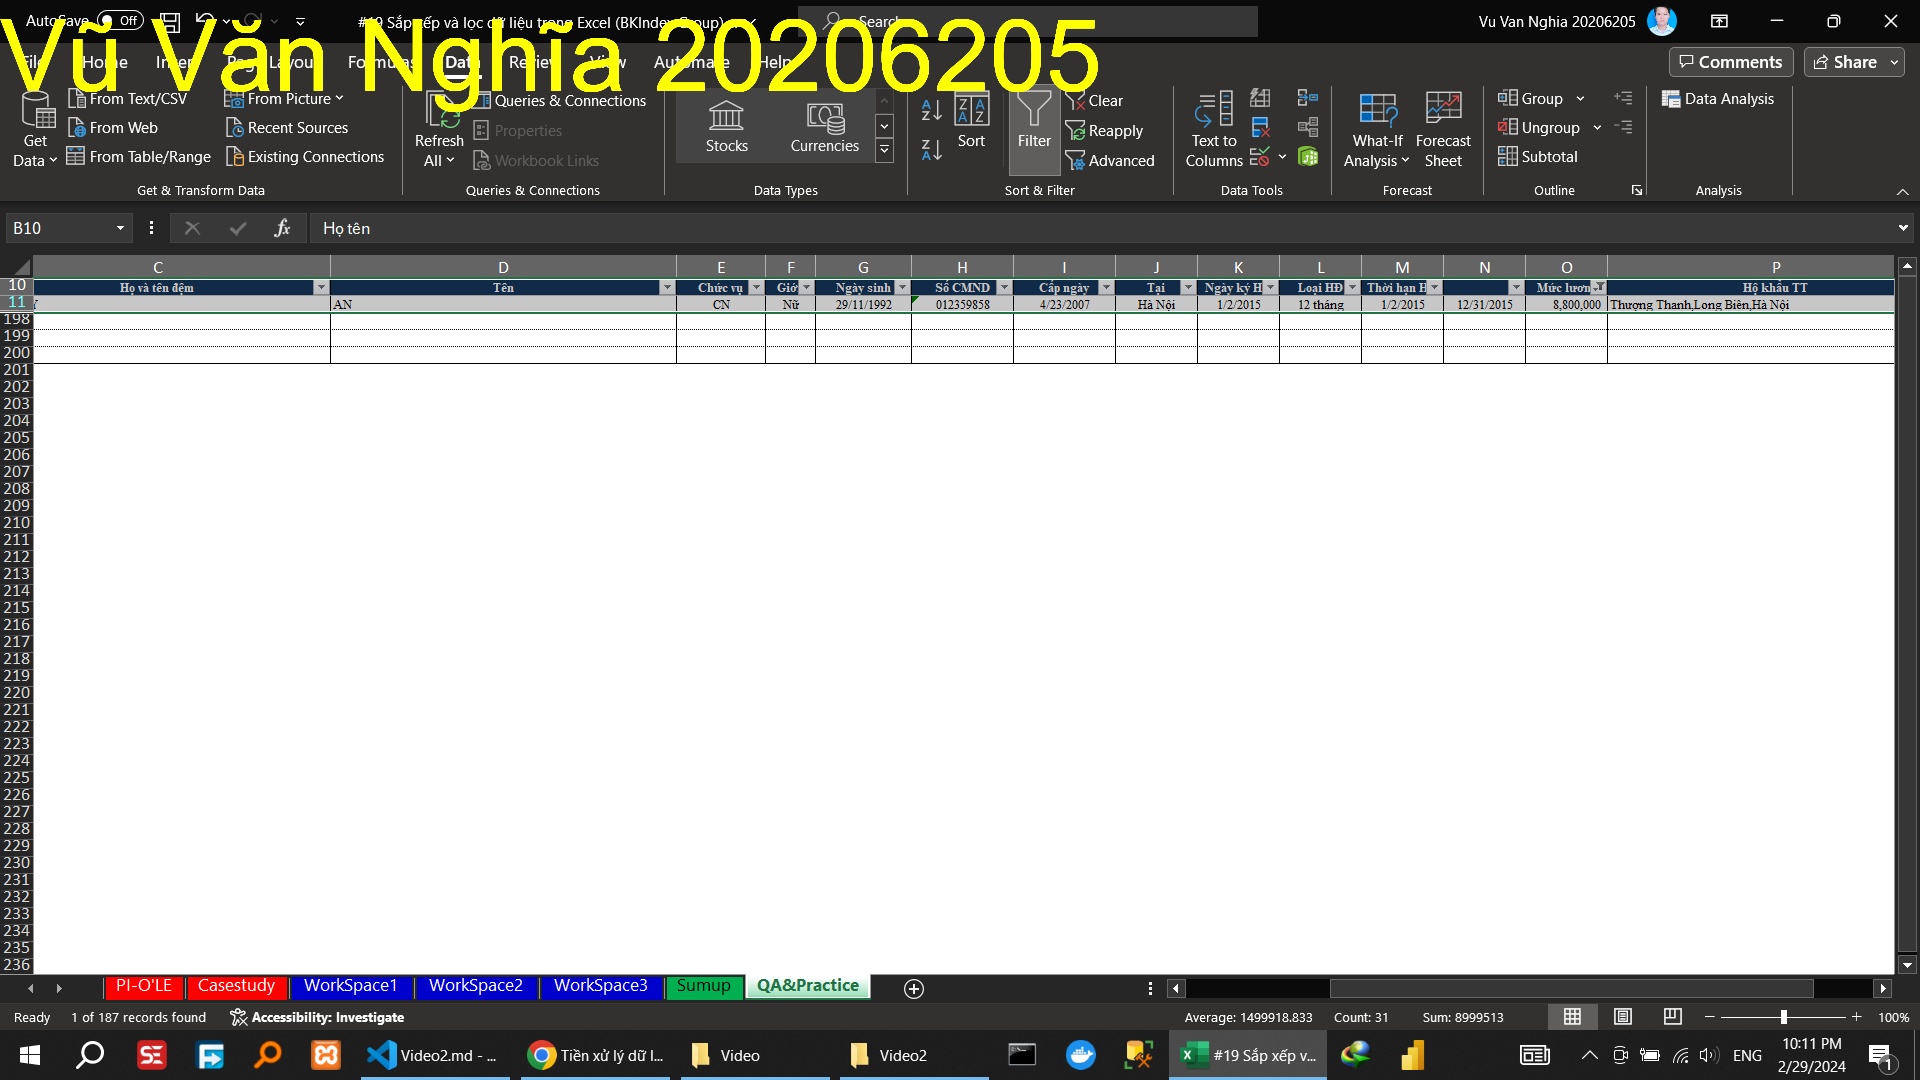
\includegraphics[scale = 0.15]{Video2/ThucHanh/4.png}
\caption{Thực hành lọc danh sách nhân viên có mức lương từ 8 đến 10 triệu}
\end{figure}

\begin{figure}[H]
\centering
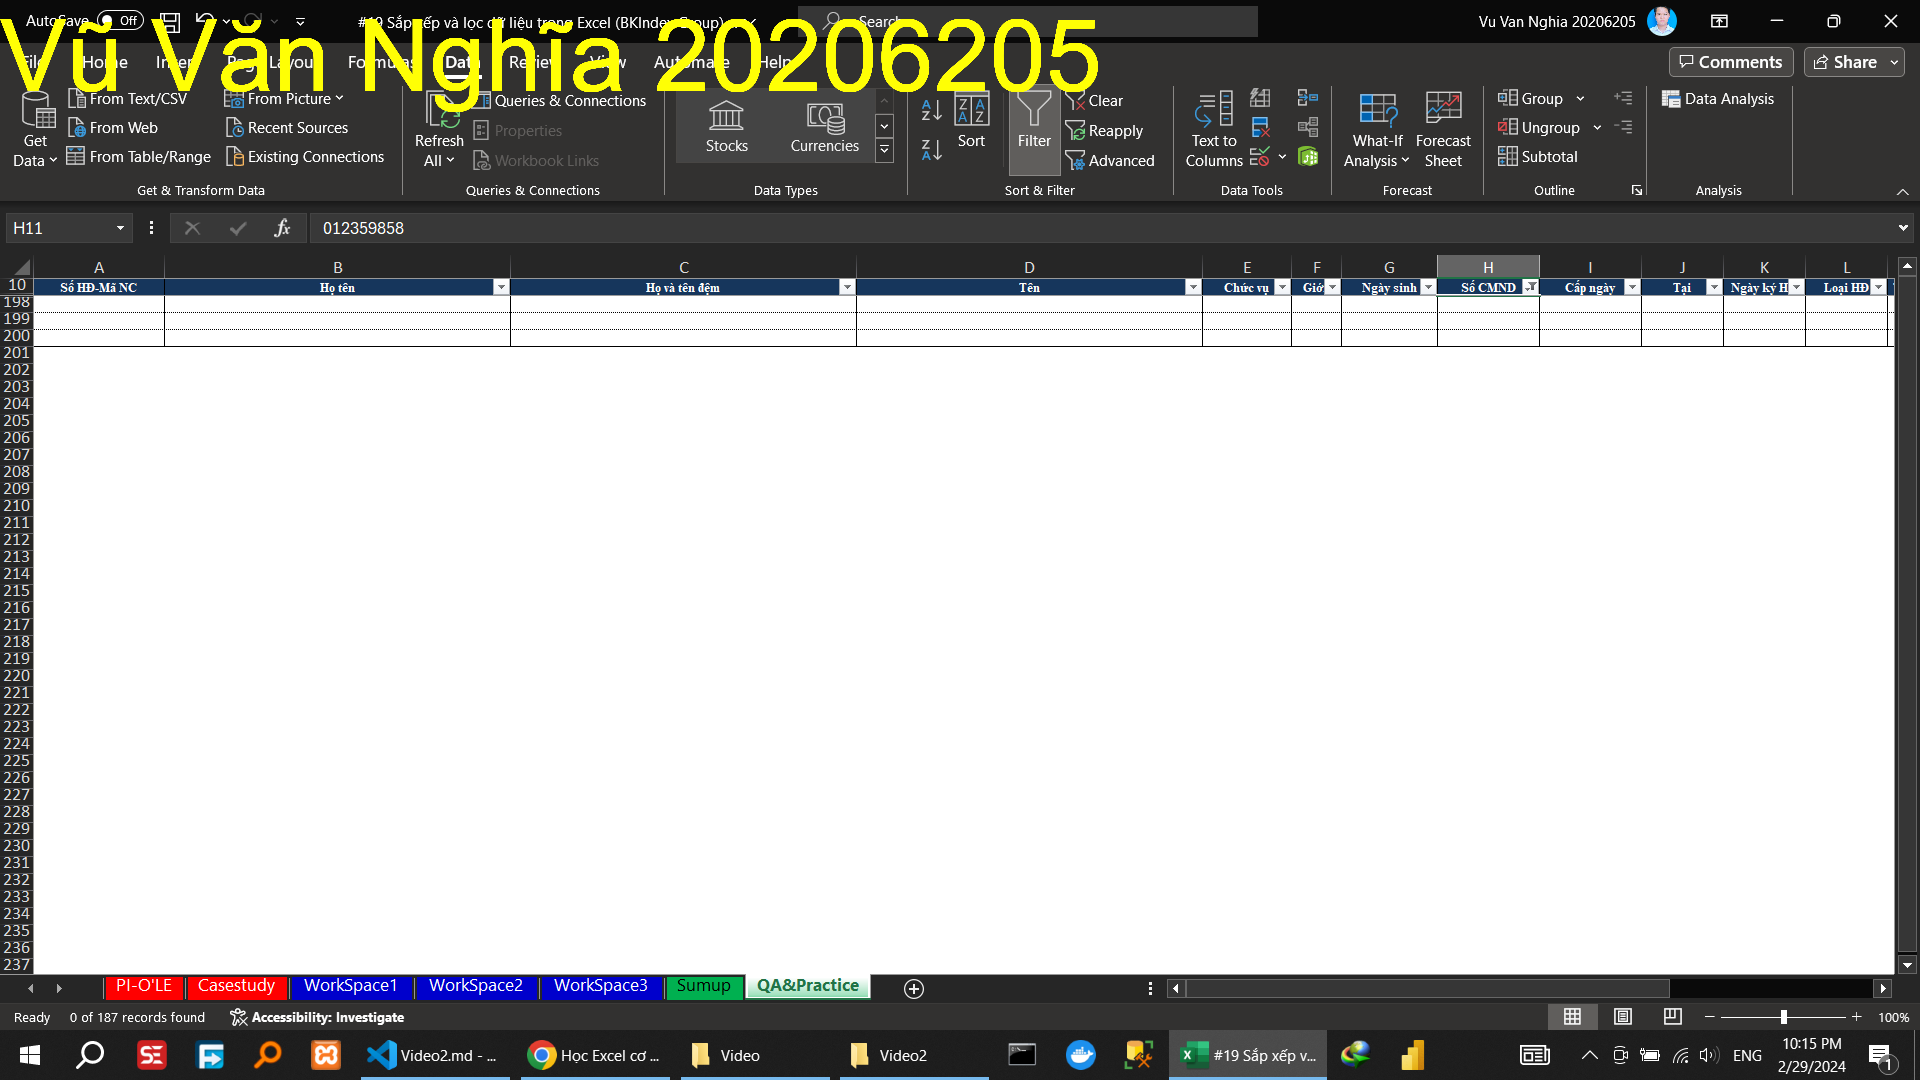
\includegraphics[scale = 0.15]{Video2/ThucHanh/5.png}
\caption{Thực hành lọc danh sách nhân viên chưa có thông tin CMND}
\end{figure}

\begin{figure}[H]
\centering
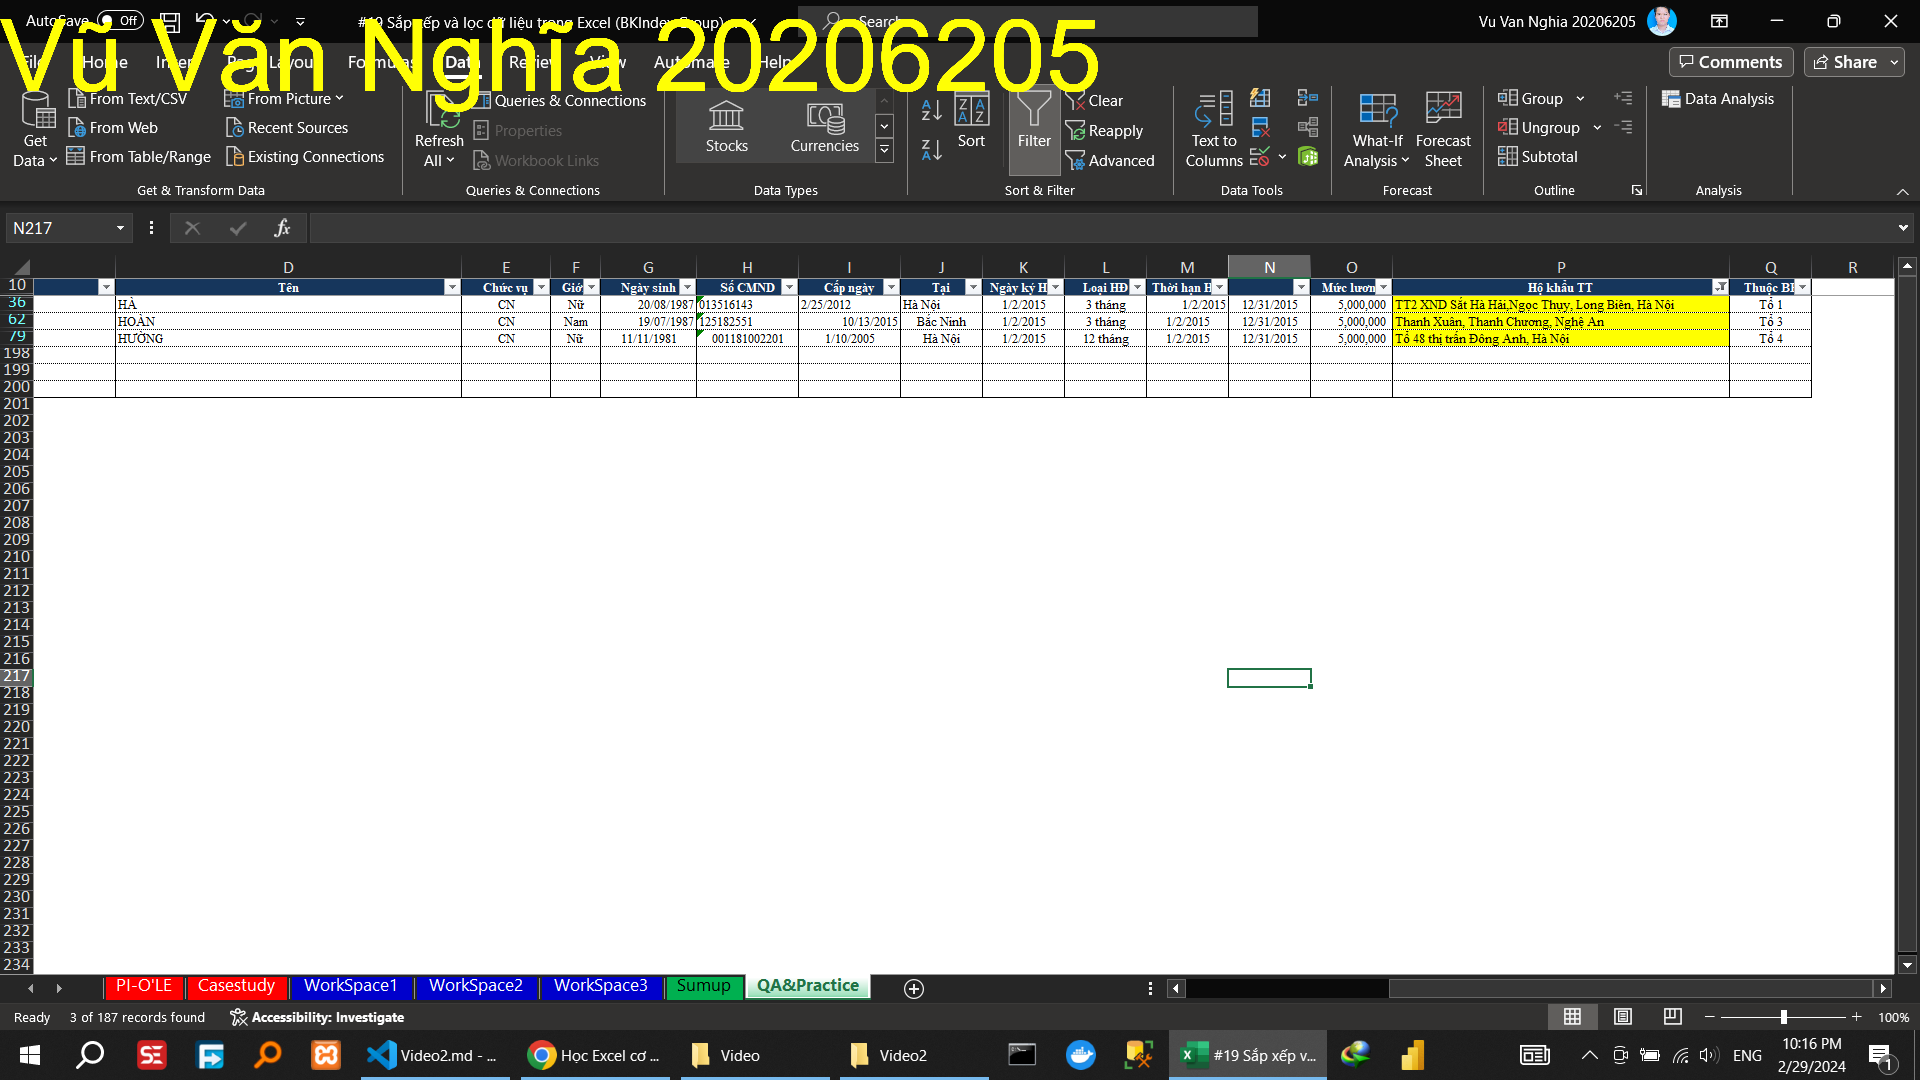
\includegraphics[scale = 0.15]{Video2/ThucHanh/6.png}
\caption{Thực hành lọc danh sách nhân viên cần xác minh lại hộ khẩu (bôi màu vàng hoặc không có thông tin hộ khẩu)}
\end{figure}

\begin{figure}[H]
\centering
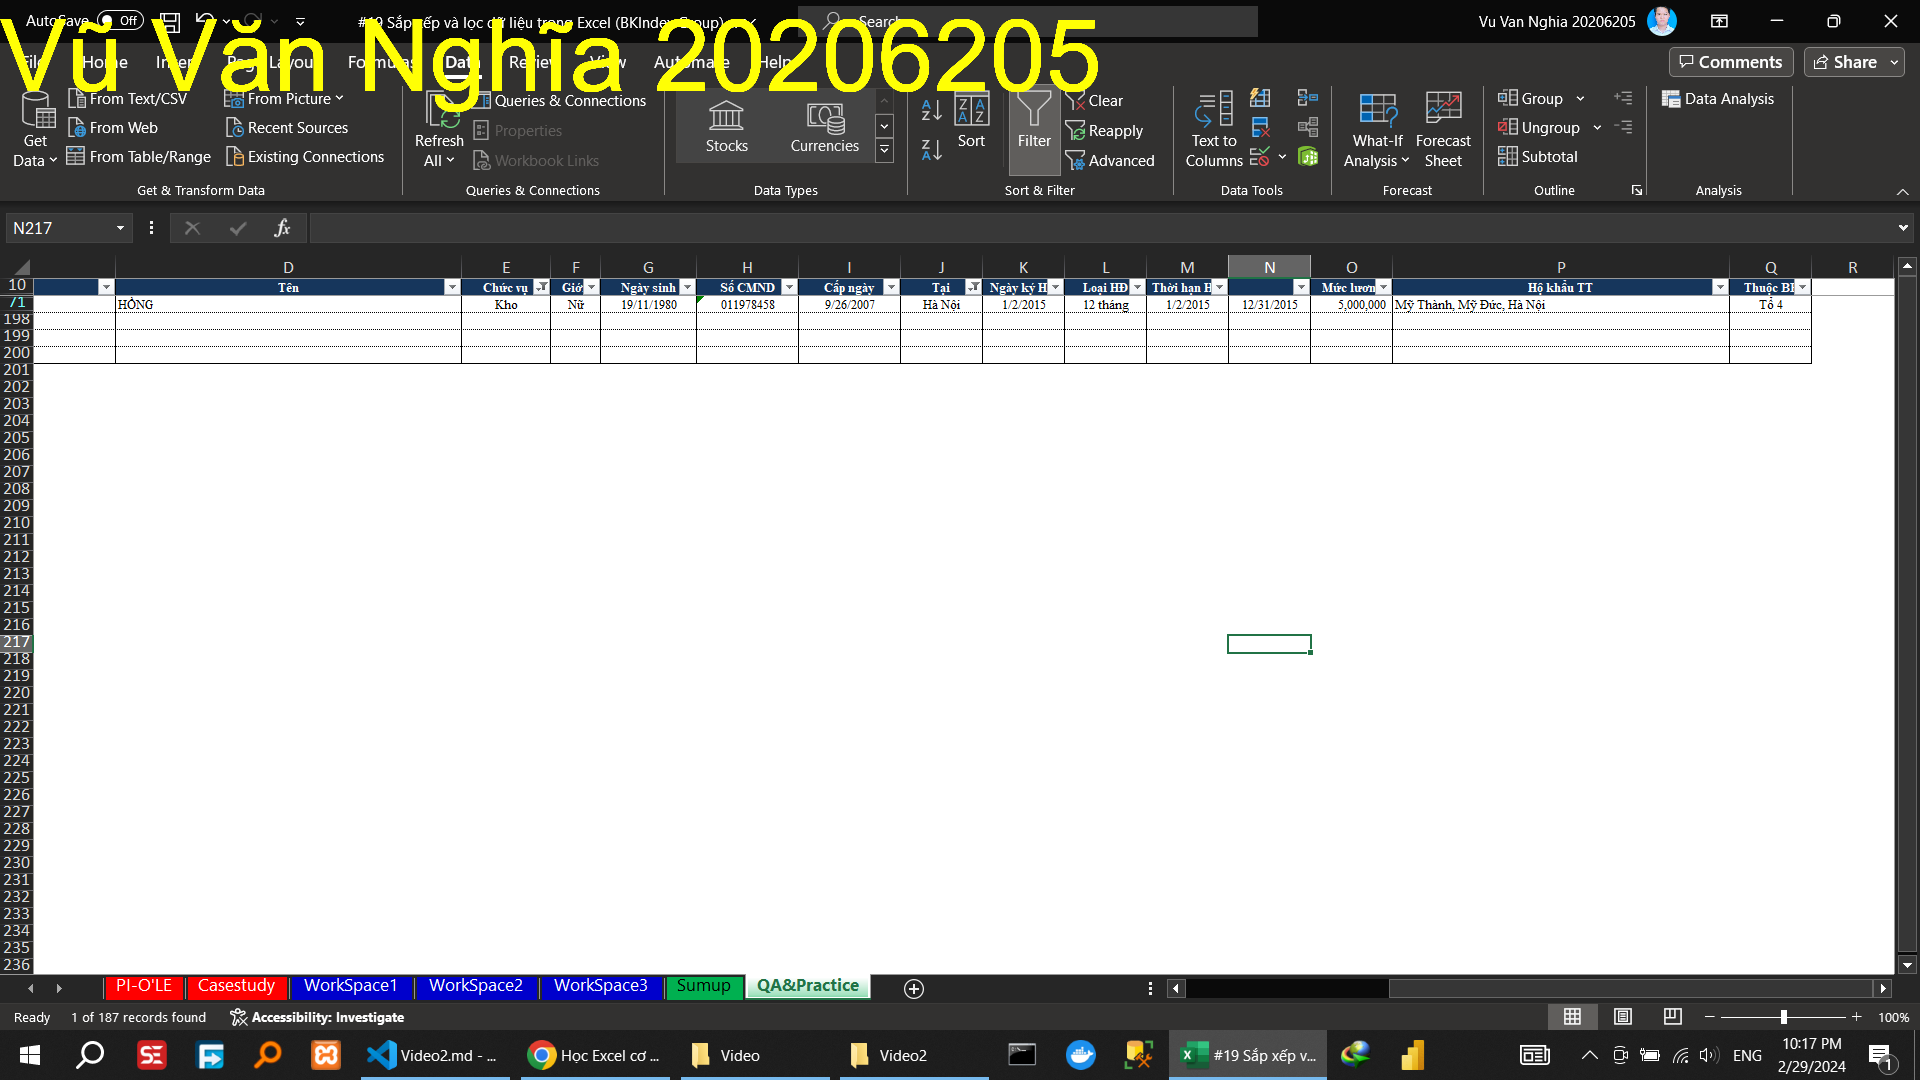
\includegraphics[scale = 0.15]{Video2/ThucHanh/7.png}
\caption{Thực hành lọc danh sách nhân viên bộ phận kho có hộ khẩu tại Hà Nội để lên lịch trực tết}
\end{figure}
%%%%%%%%%%%%%%%%%%%%%%%%%%%%%%%%%%%%%%%%%%%%%%%%%%%%%%%
\subsection{Video 3}
%%%%%%%%%%%%%%%%%%%%%%%%%%%%%%%%%%%%%%%%%%%%%%%%%%%%%%%
\begin{figure}[H]
\centering
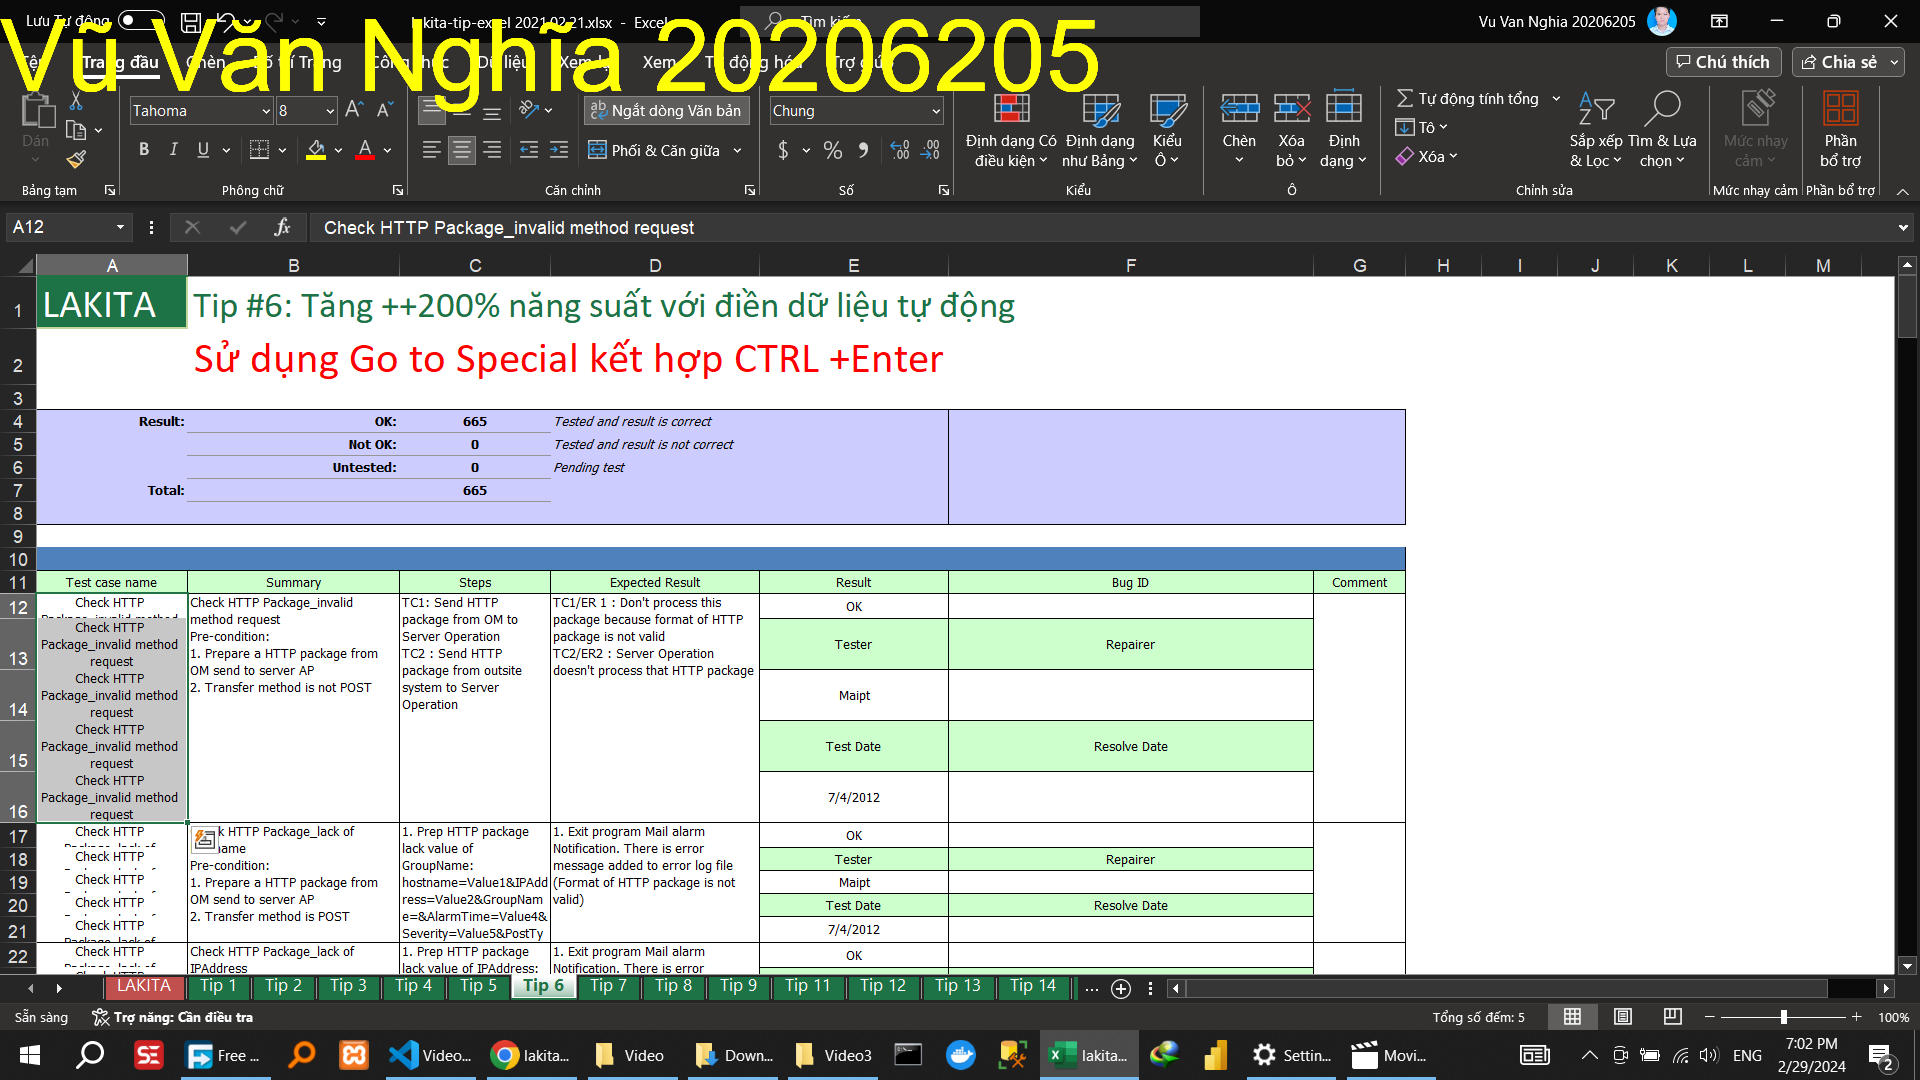
\includegraphics[scale = 0.15]{Video3/HuongDan/1.png}
\caption{Hướng dẫn tự động điền thông tin vùng trống}
\end{figure}
%%%%%%%%%%%%%%%%%%%%%%%%%%%%%%%%%%%%%%%%%%%%%%%%%%%%%%
\subsection{Video 4}
%%%%%%%%%%%%%%%%%%%%%%%%%%%%%%%%%%%%%%%%%%%%%%%%%%%%%%%
\begin{figure}[H]
\centering
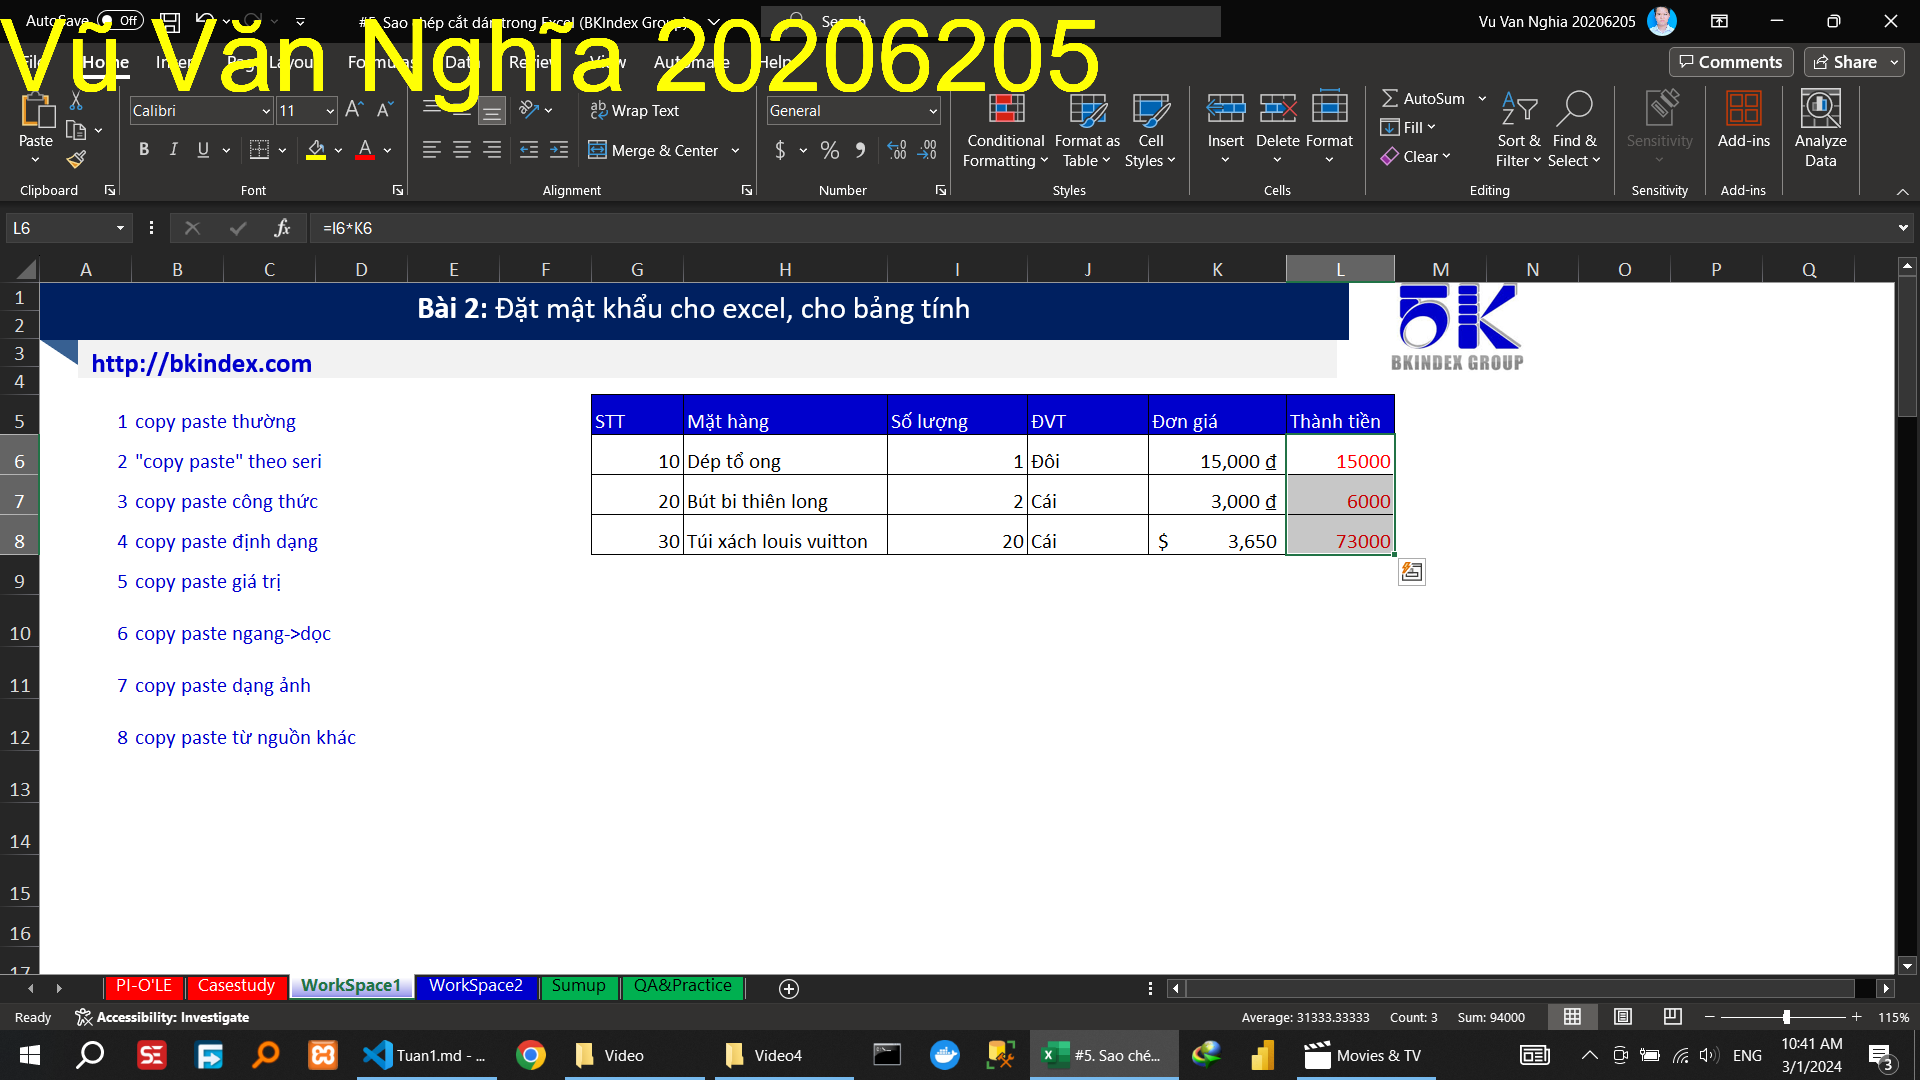
\includegraphics[scale = 0.15]{Video4/HuongDan/0.png}
\caption{Hướng dẫn sao chép thông thường cột thành tiền}
\end{figure}

\begin{figure}[H]
\centering
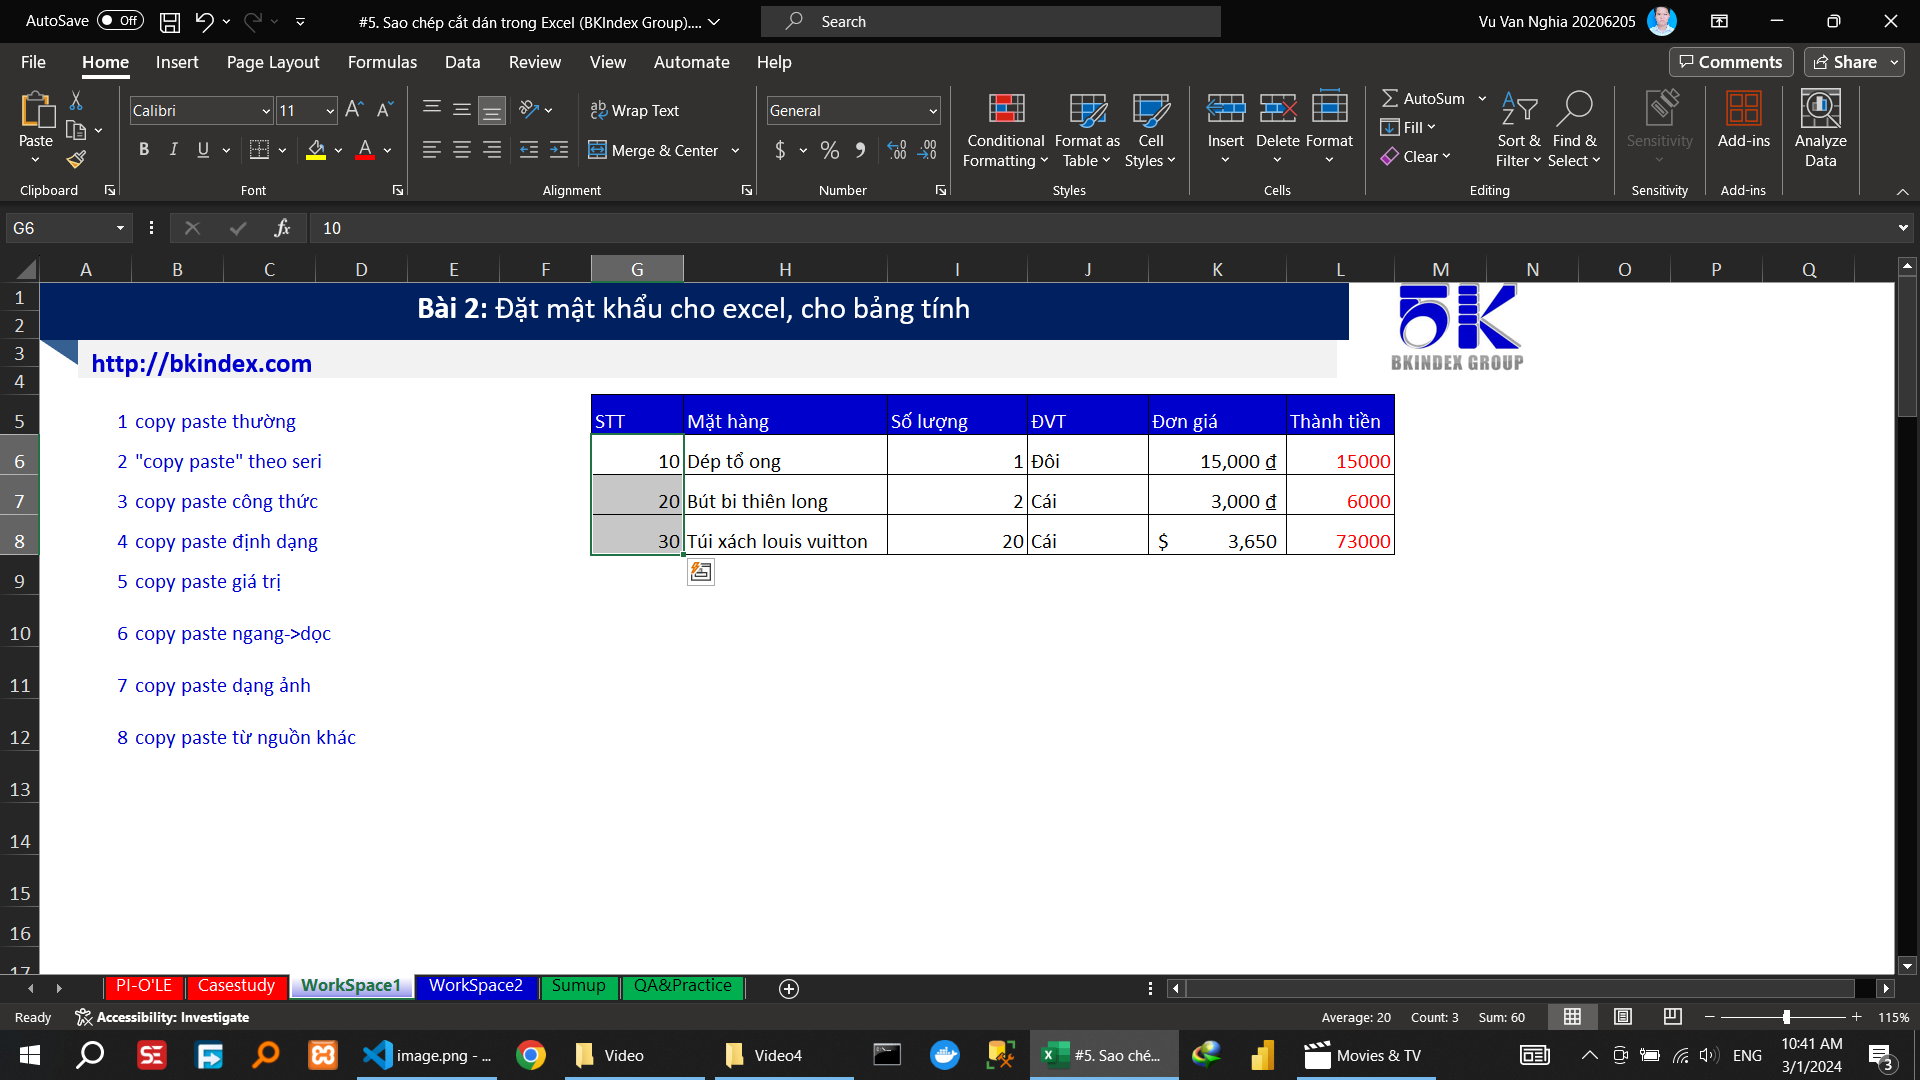
\includegraphics[scale = 0.15]{Video4/HuongDan/1.png}
\caption{Hướng dẫn sao chép theo seri số thứ tự}
\end{figure}

\begin{figure}[H]
\centering
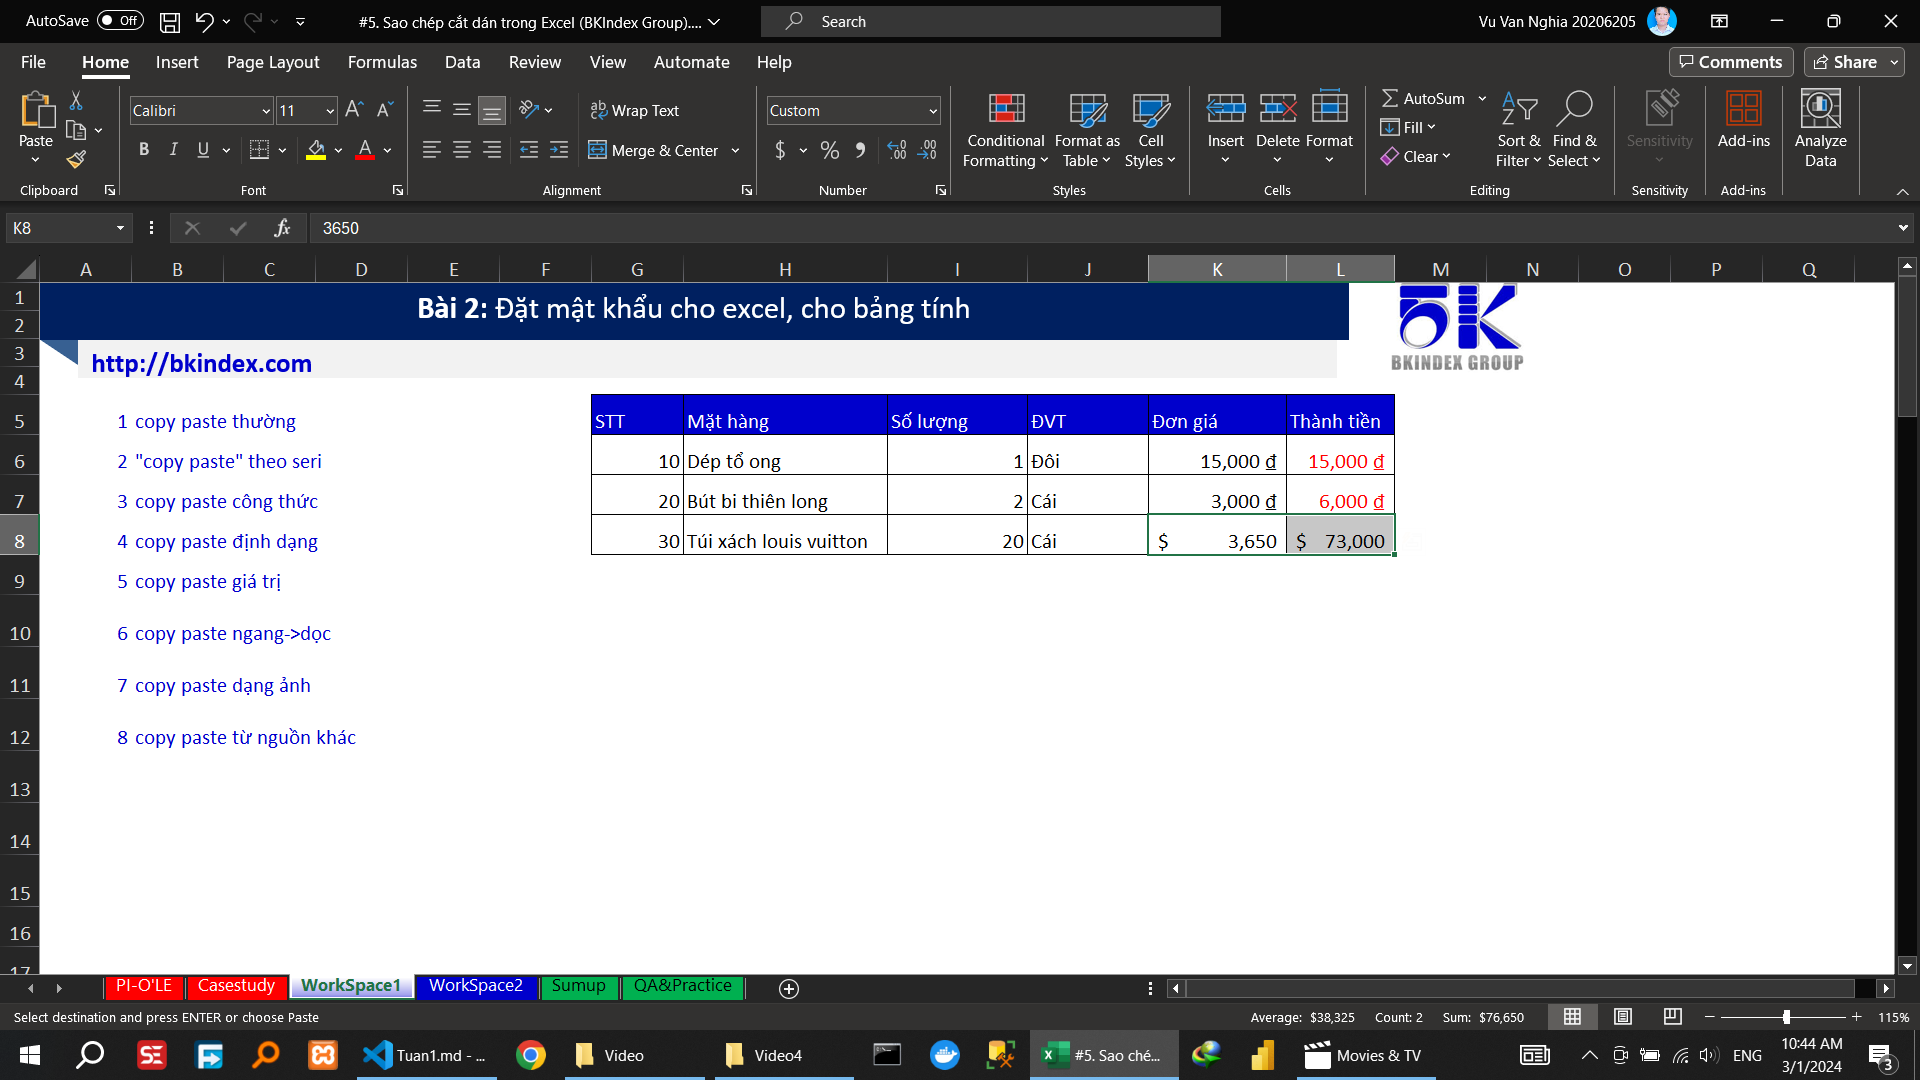
\includegraphics[scale = 0.15]{Video4/HuongDan/2.png}
\caption{Hướng dẫn sao chép công thức thành tiền}
\end{figure}

\begin{figure}[H]
\centering
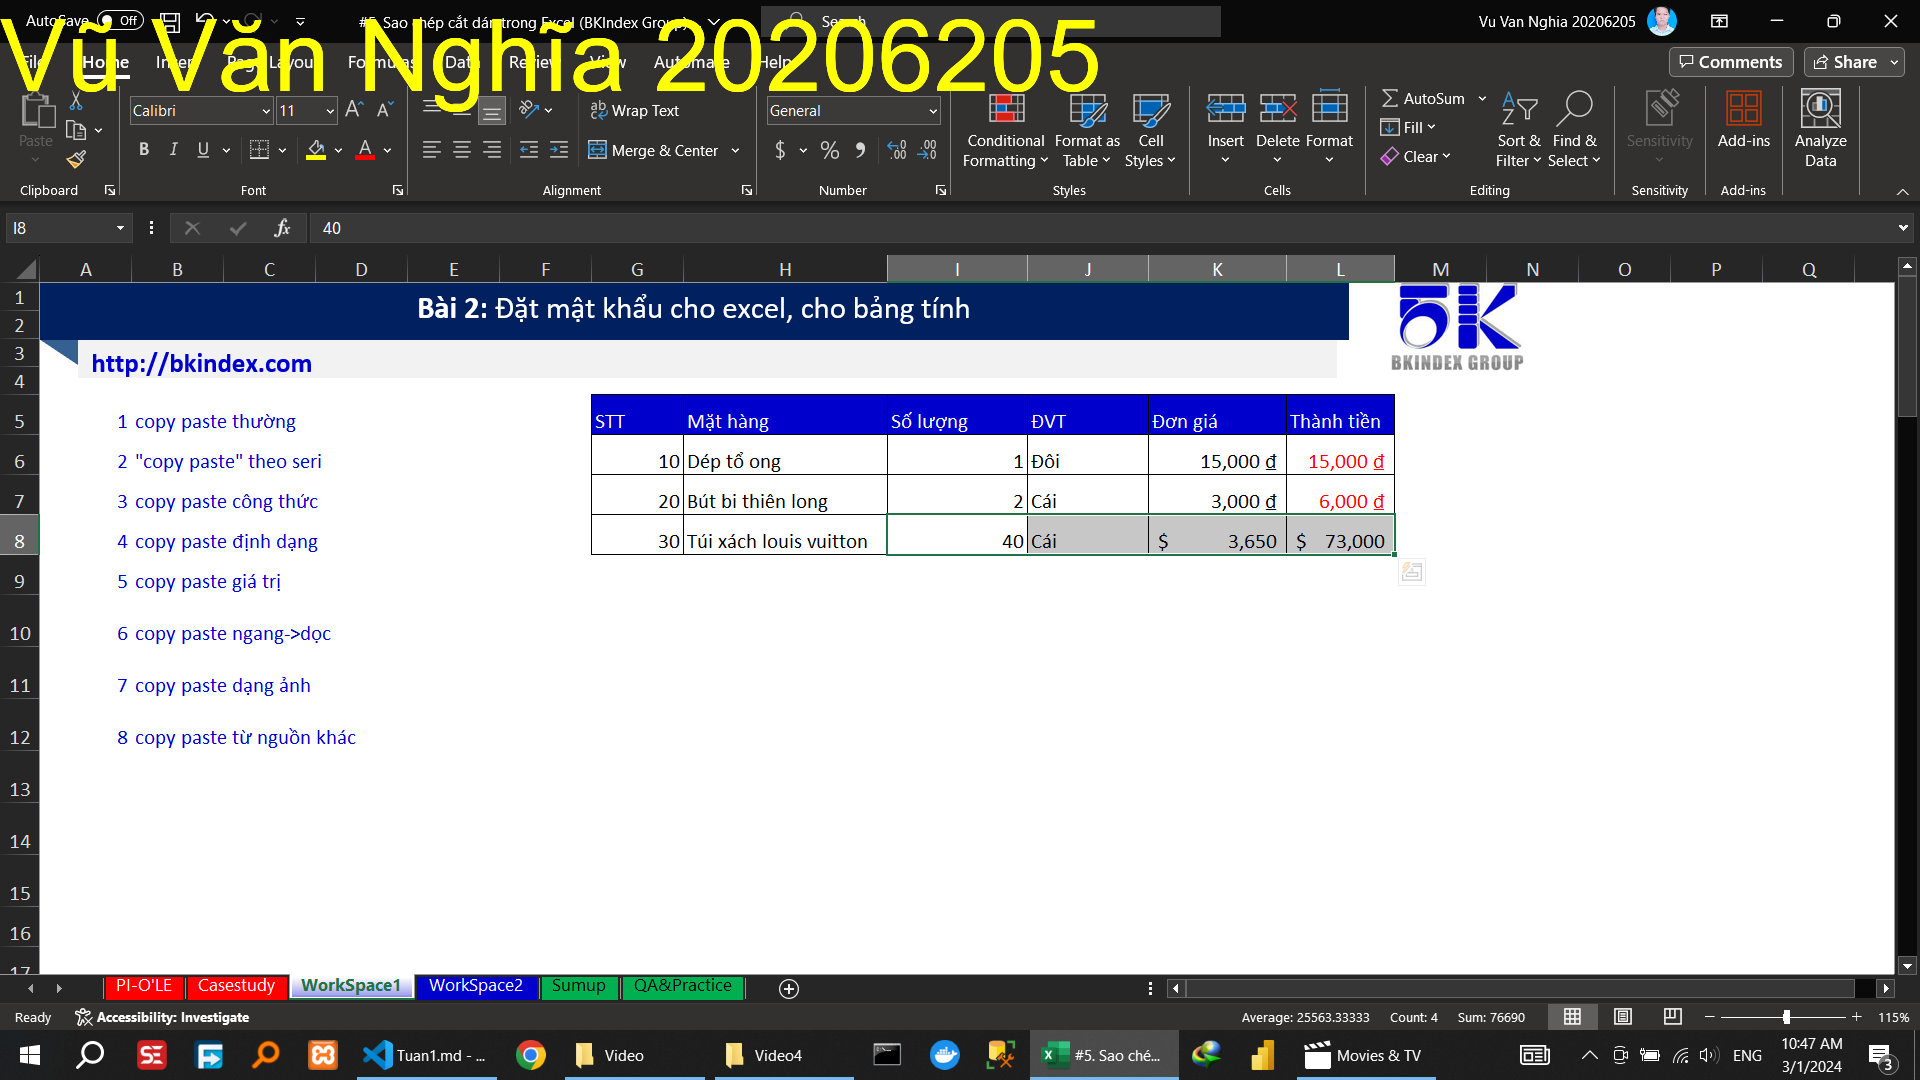
\includegraphics[scale = 0.15]{Video4/HuongDan/3.png}
\caption{Hướng dẫn sao chép giá trị thành tiền}
\end{figure}

\begin{figure}[H]
\centering
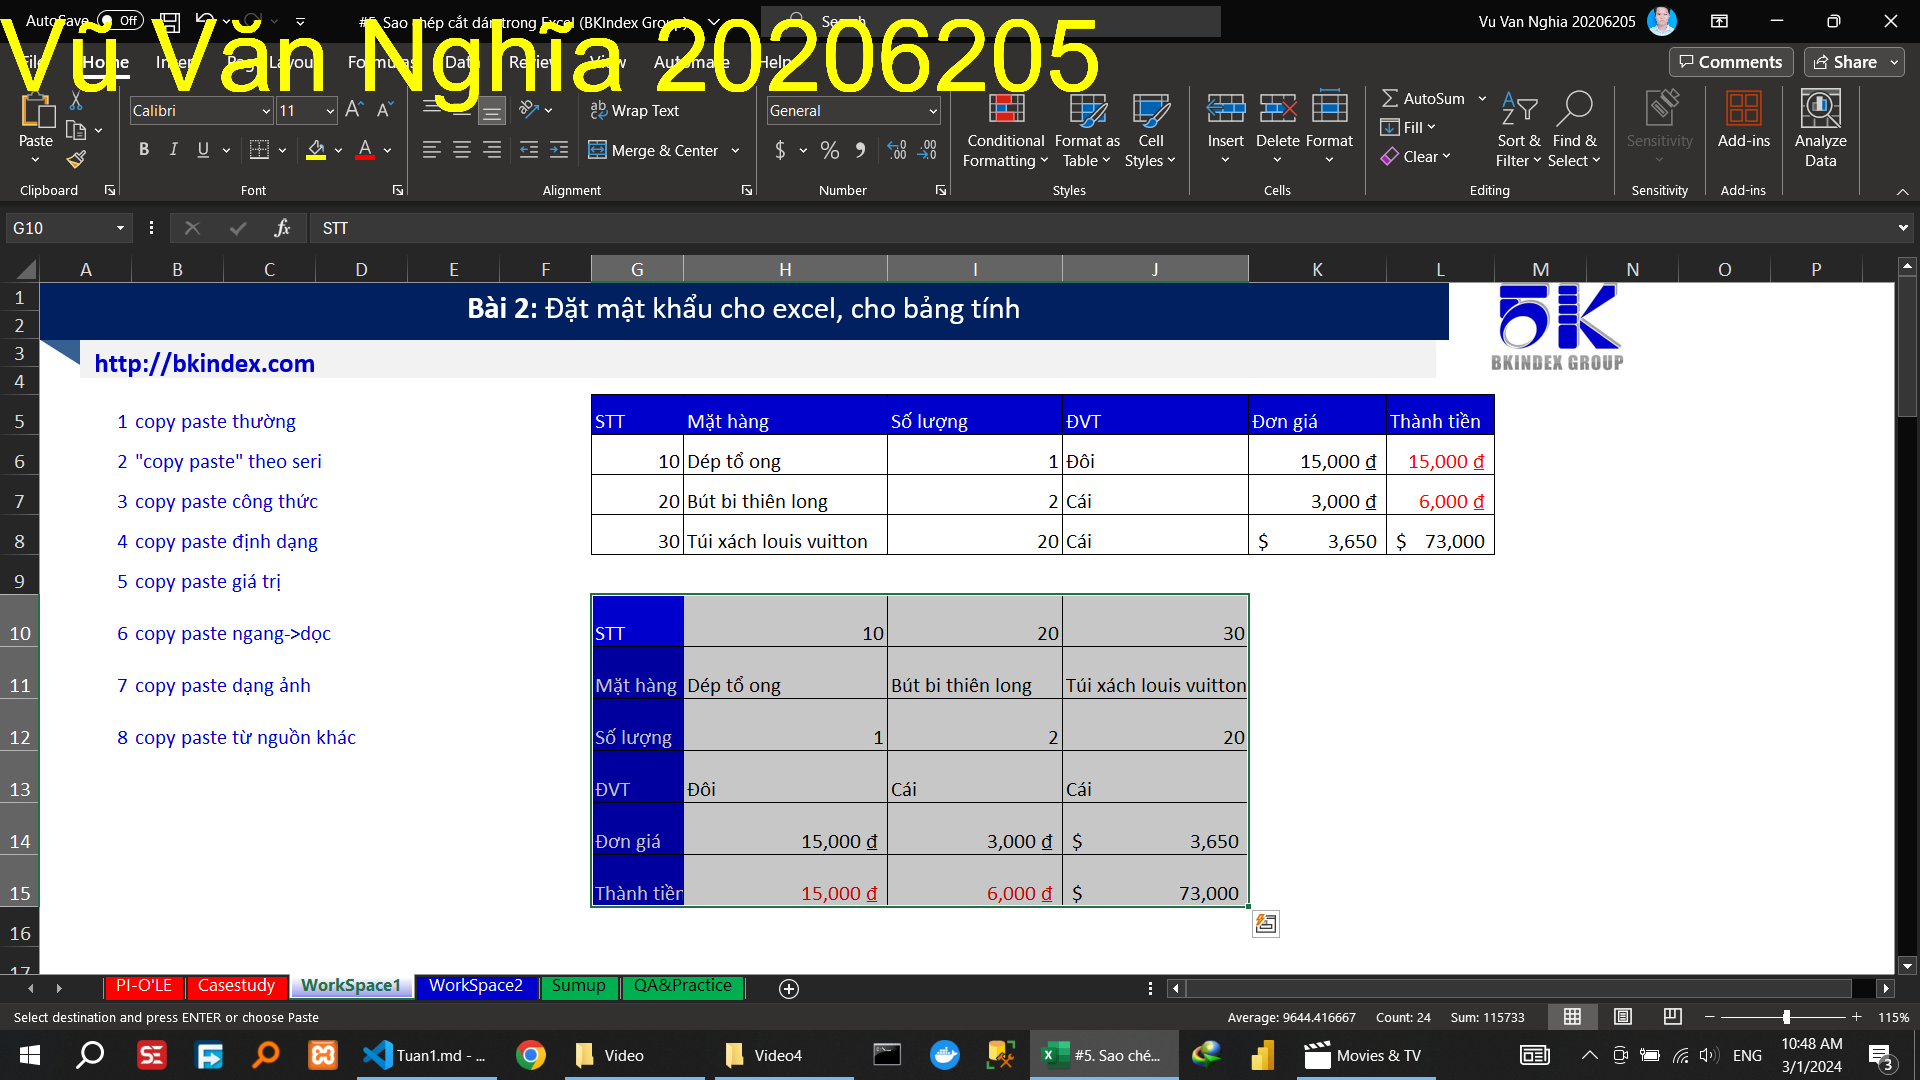
\includegraphics[scale = 0.15]{Video4/HuongDan/4.png}
\caption{Hướng dẫn sao chép ngang thành dọc}
\end{figure}

\begin{figure}[H]
\centering
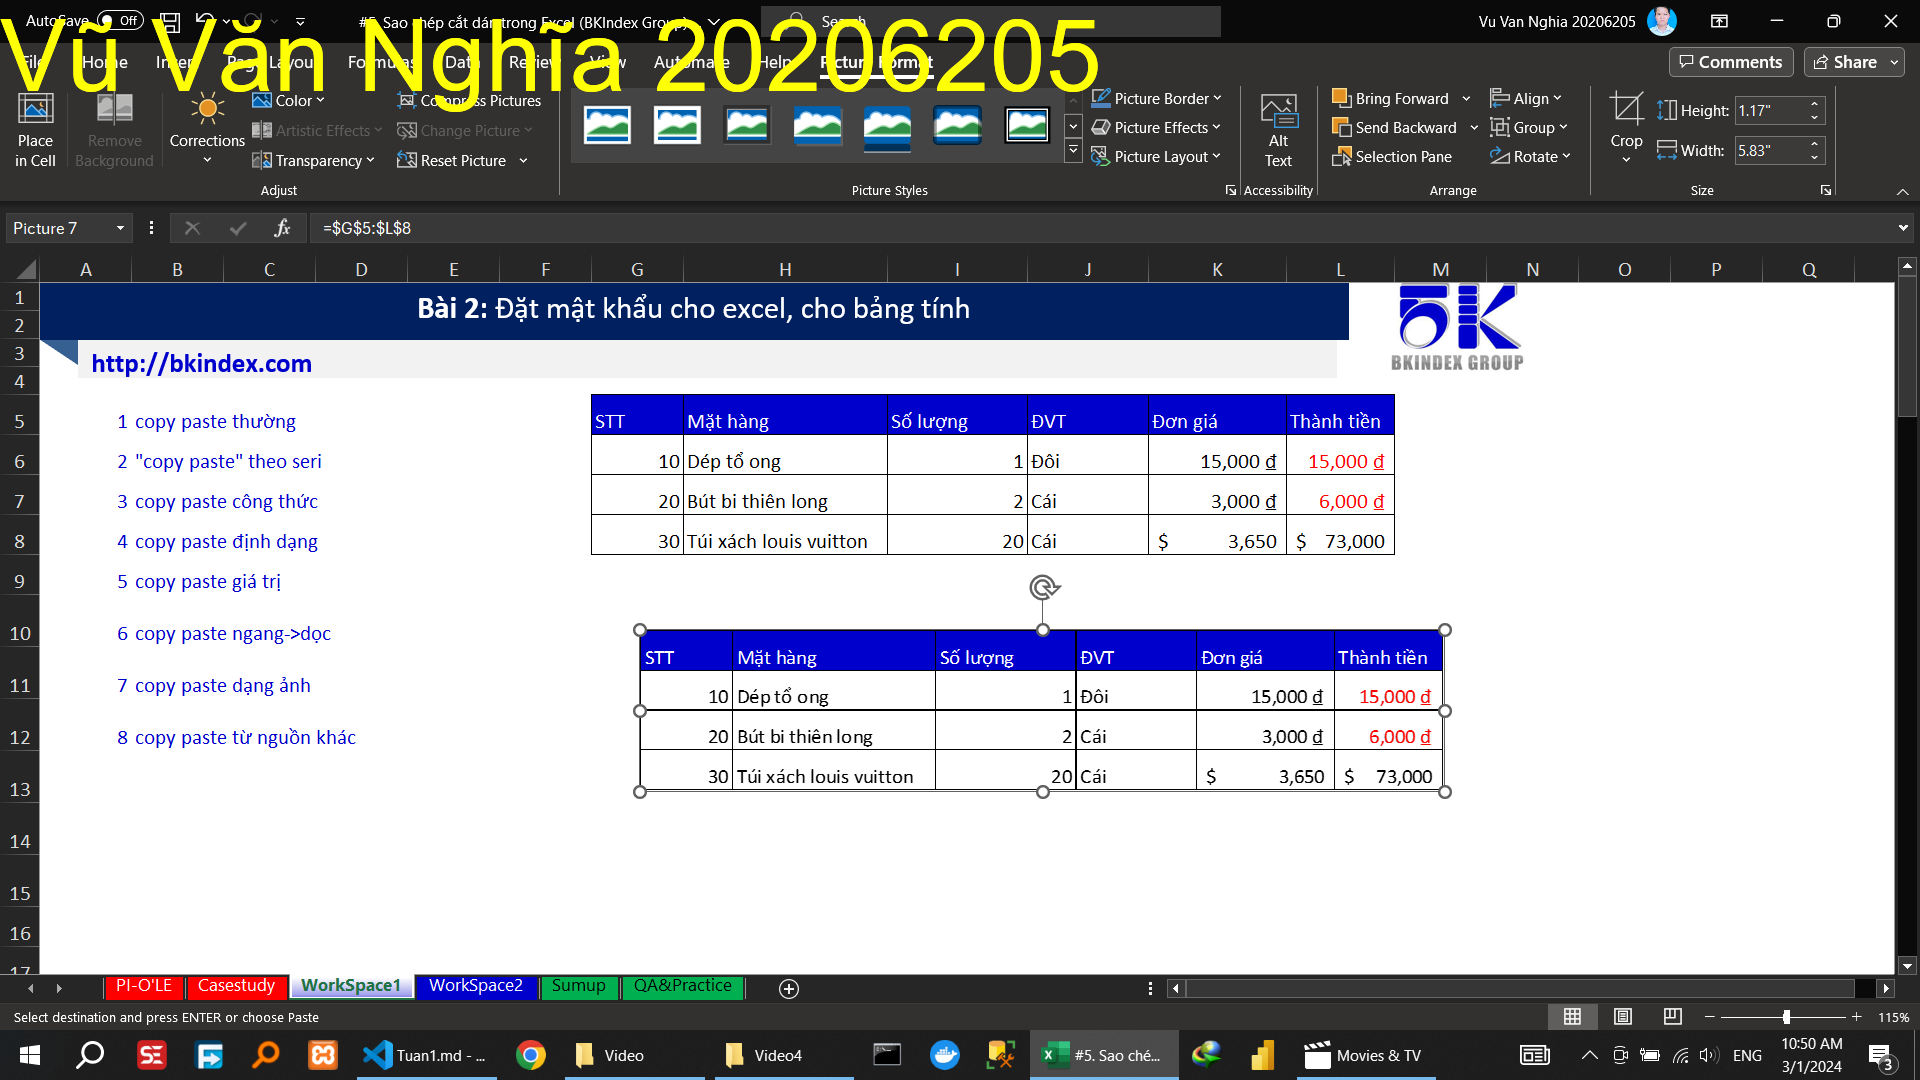
\includegraphics[scale = 0.15]{Video4/HuongDan/5.png}
\caption{Hướng dẫn sao chép dạng ảnh}
\end{figure}

\begin{figure}[H]
\centering
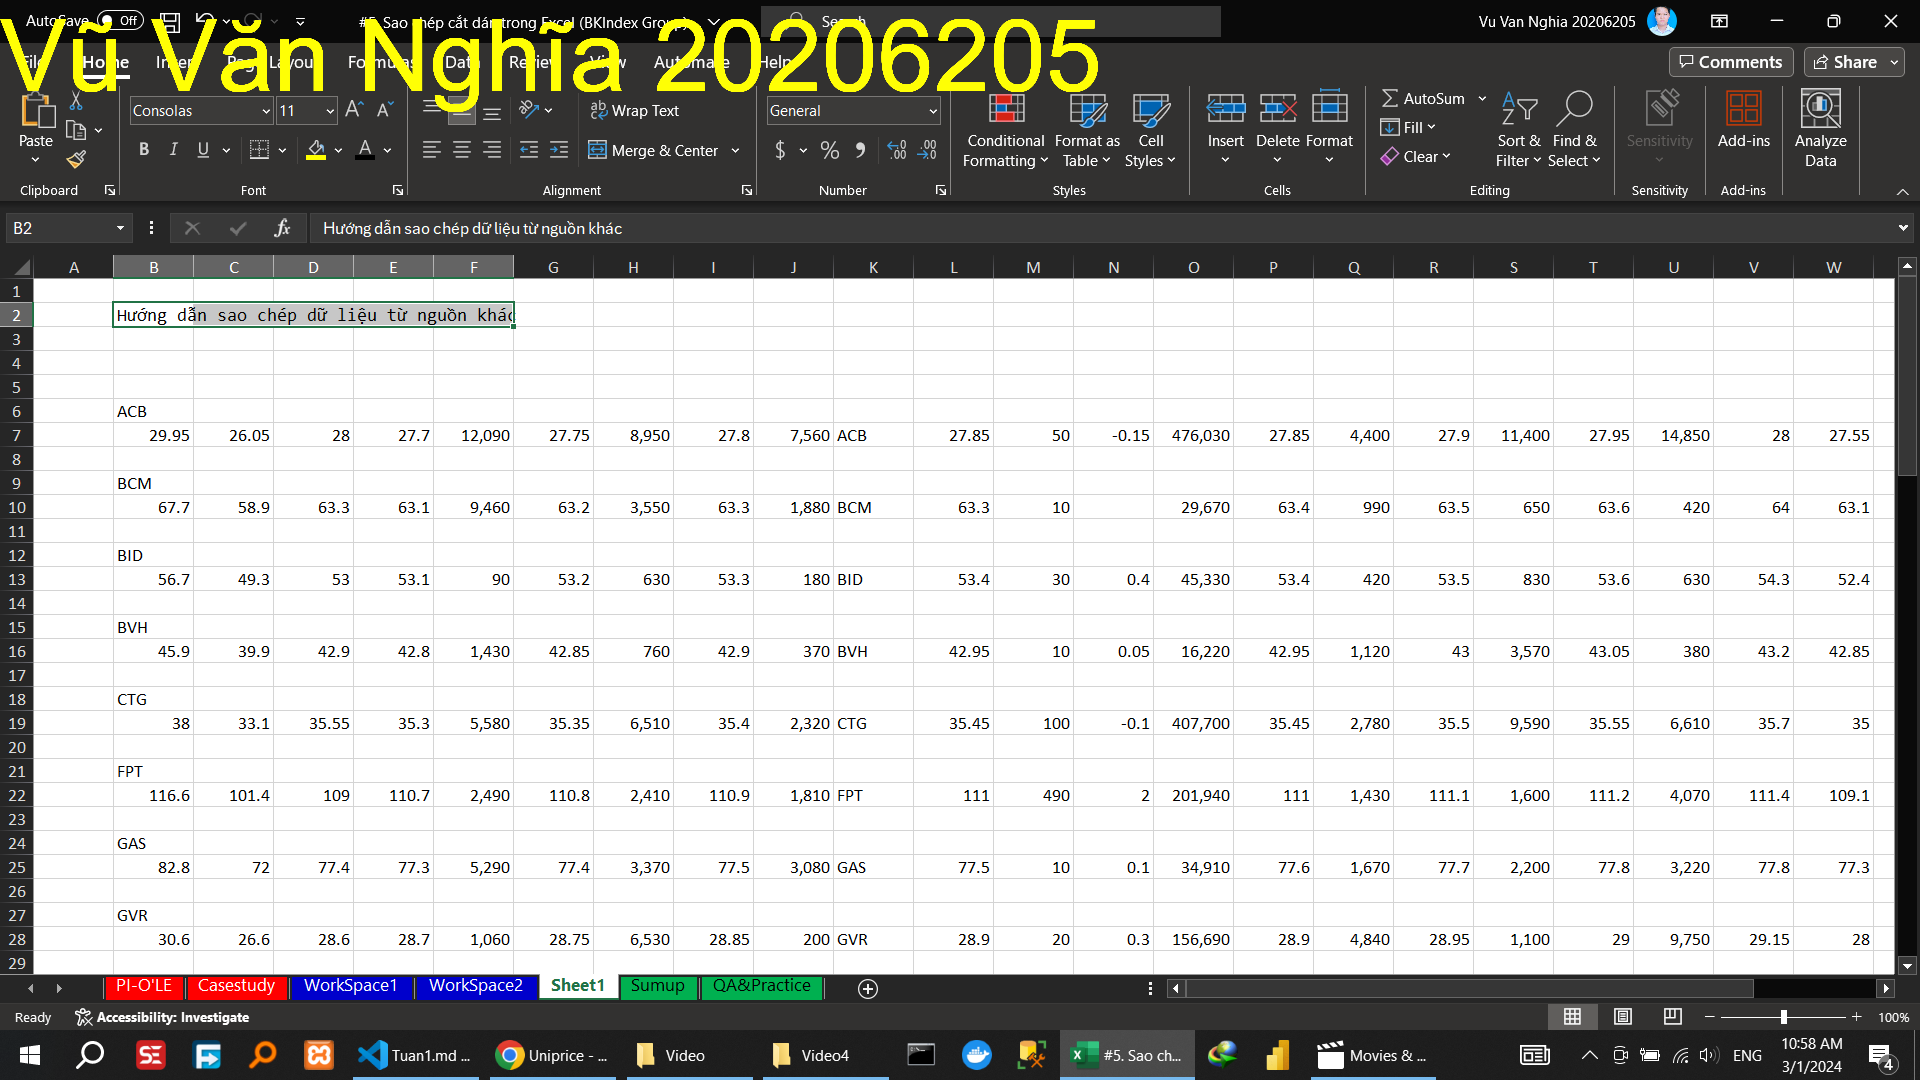
\includegraphics[scale = 0.15]{Video4/HuongDan/6.png}
\caption{Hướng dẫn sao chép dữ liệu từ nguồn khác}
\end{figure}
%%%%%%%%%%%%%%%%%%%%%%%%%%%%%%%%%%%%%%%%%%%%%%%%%%%%%%
\begin{figure}[H]
\centering
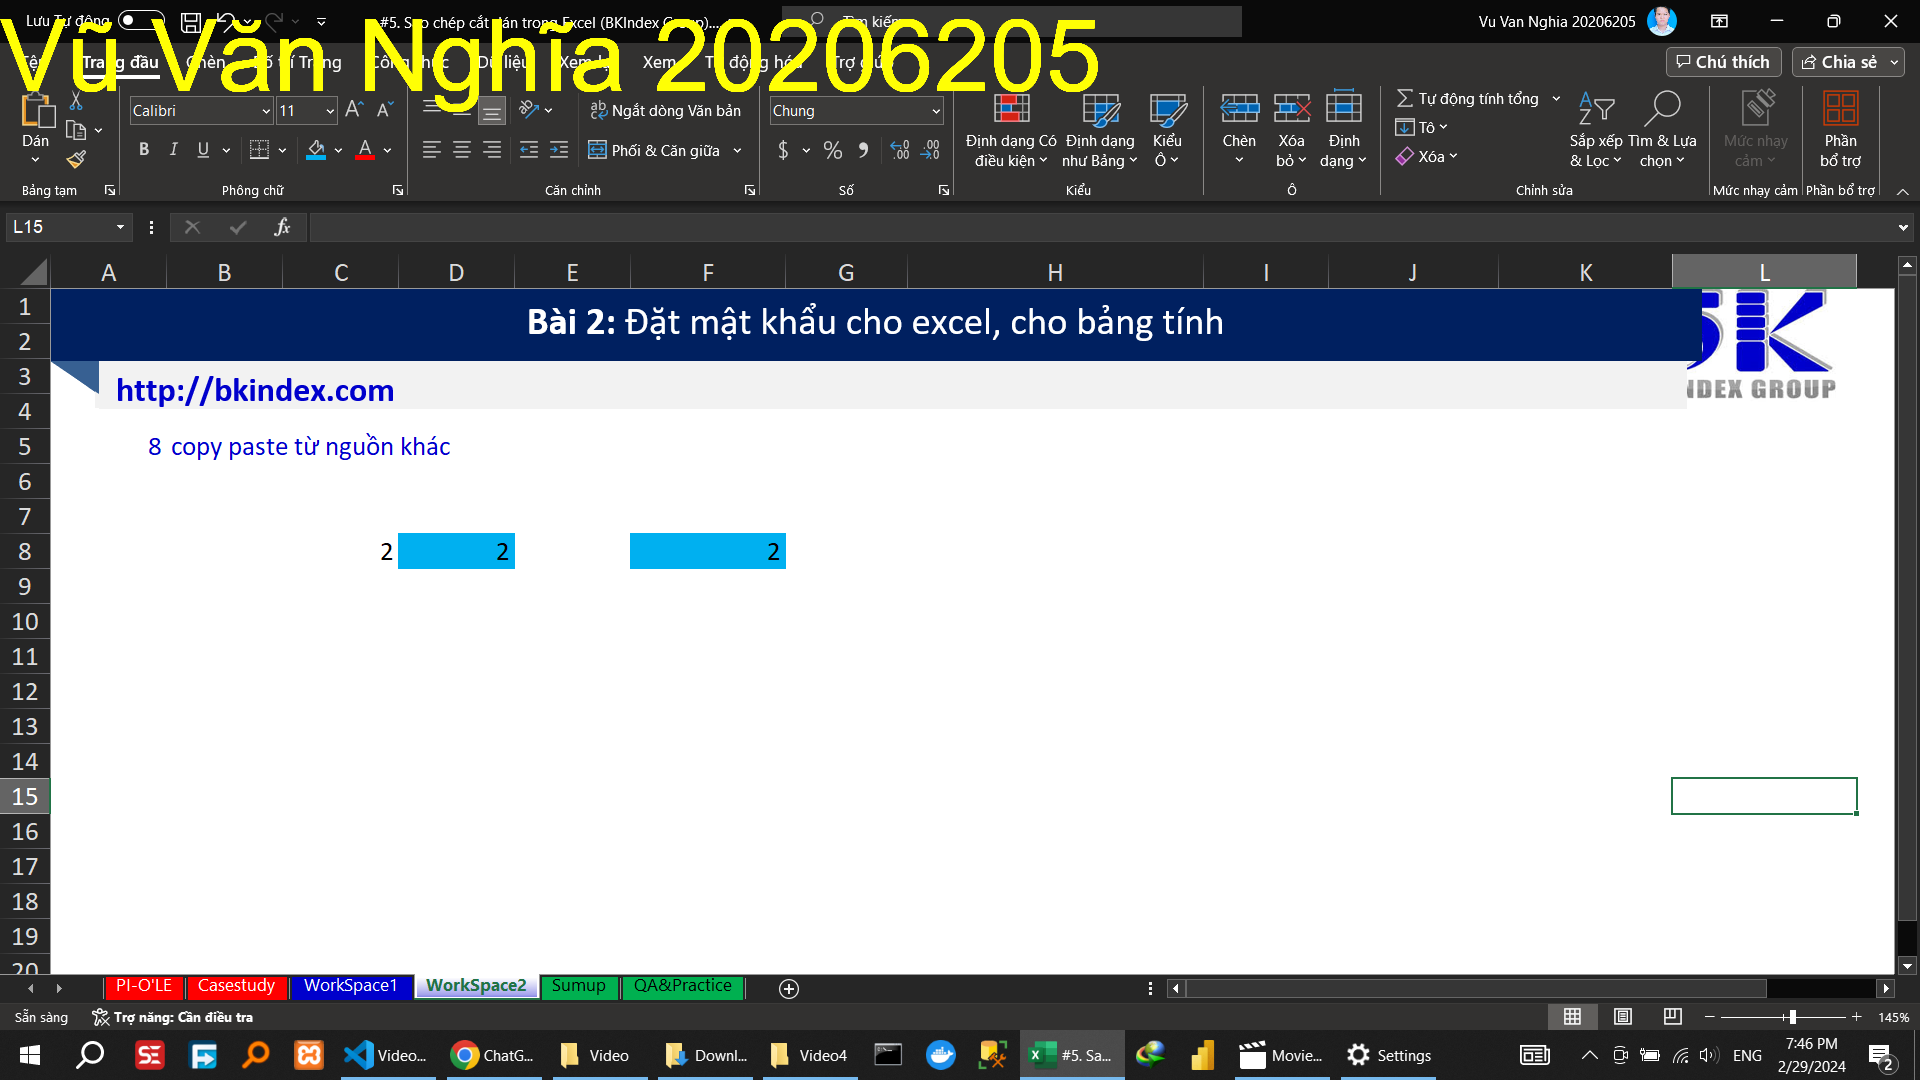
\includegraphics[scale = 0.15]{Video4/ThucHanh/1.png}
\caption{Thực hành đổi tên tiêu đề và sao chép giá trị, màu sắc}
\end{figure}
%%%%%%%%%%%%%%%%%%%%%%%%%%%%%%%%%%%%%%%%%%%%%%%%%%%%%%
\subsection{Video 5}
%%%%%%%%%%%%%%%%%%%%%%%%%%%%%%%%%%%%%%%%%%%%%%%%%%%%%
\begin{figure}[H]
\centering
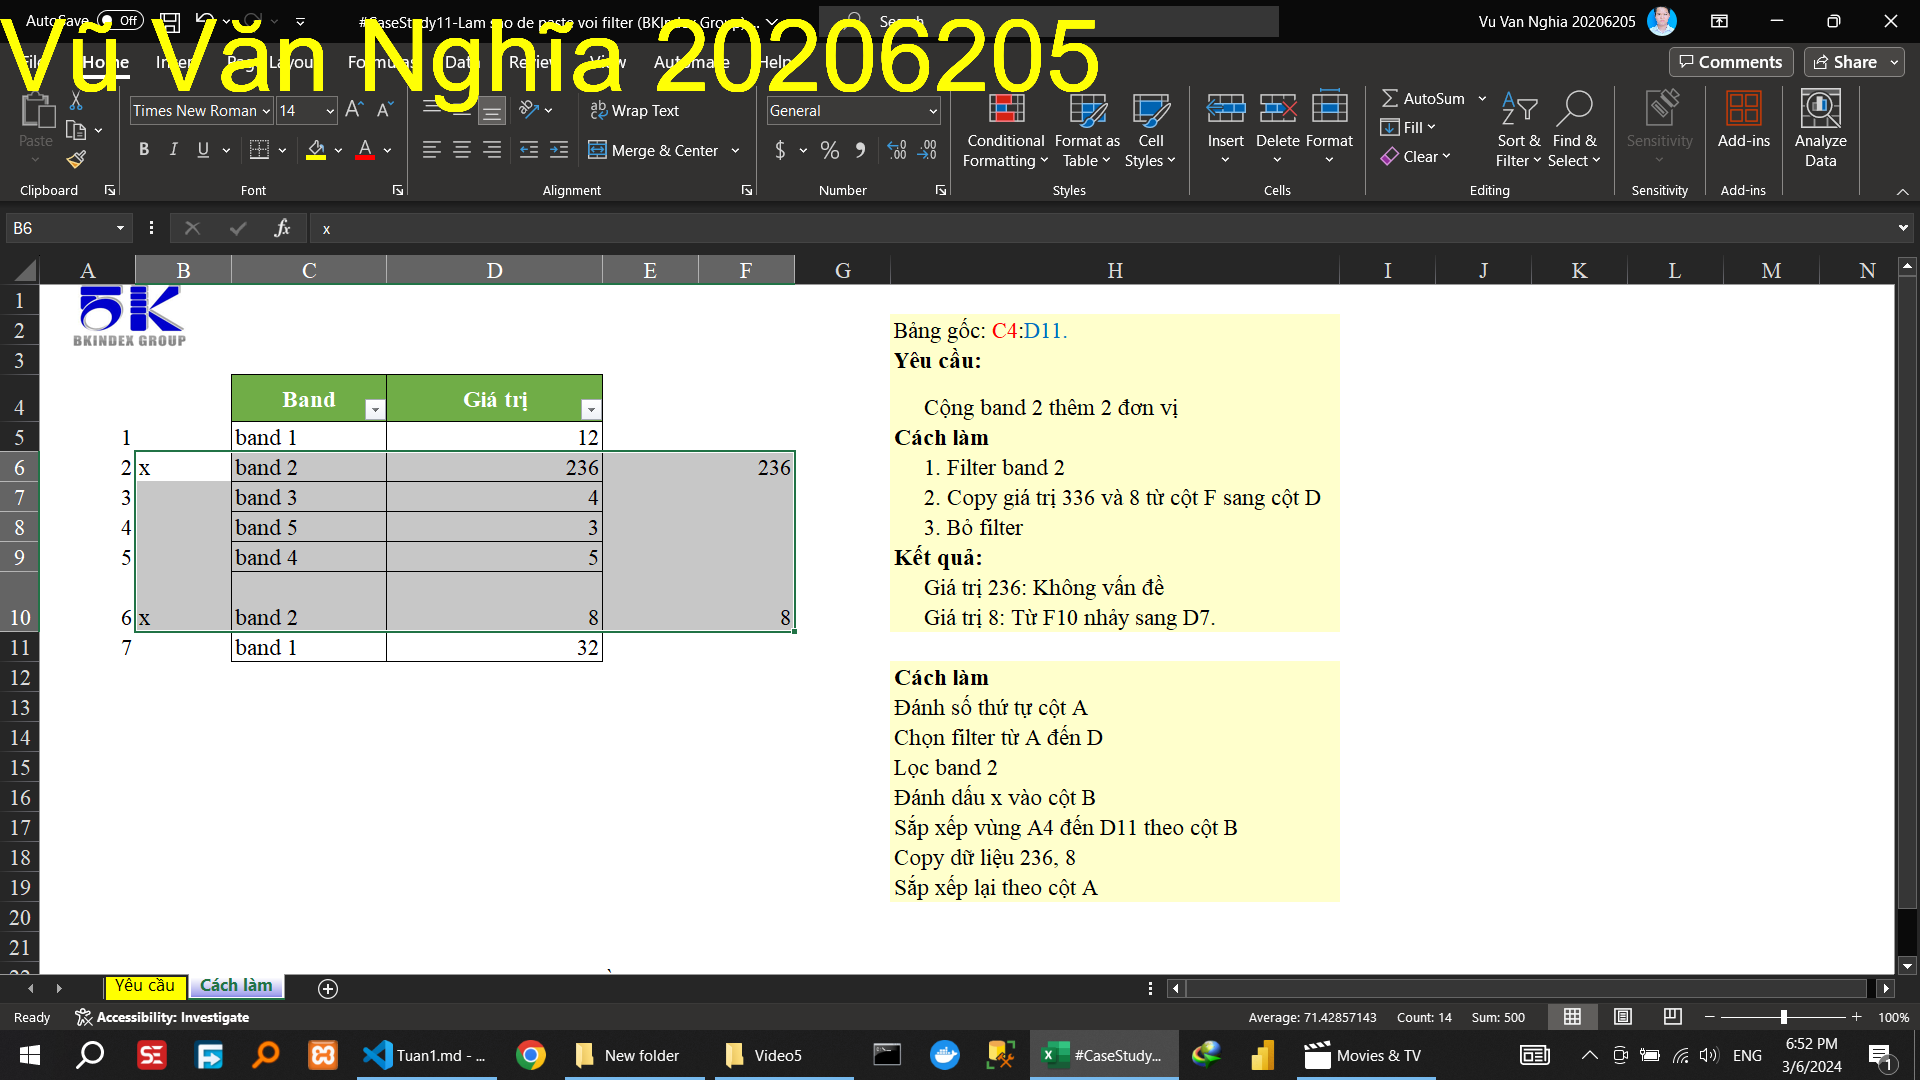
\includegraphics[scale = 0.15]{Video5/HuongDan/0.png}
\caption{Hướng dẫn dán vào vùng dữ liệu đã được filter}
\end{figure}
% %%%%%%%%%%%%%%%%%%%%%%%%%%%%%%%%%%%%%%%%%%%%%%%%%%%%%
\subsection{Video 6}
%%%%%%%%%%%%%%%%%%%%%%%%%%%%%%%%%%%%%%%%%%%%%%%%%%%
\begin{figure}[H]
\centering
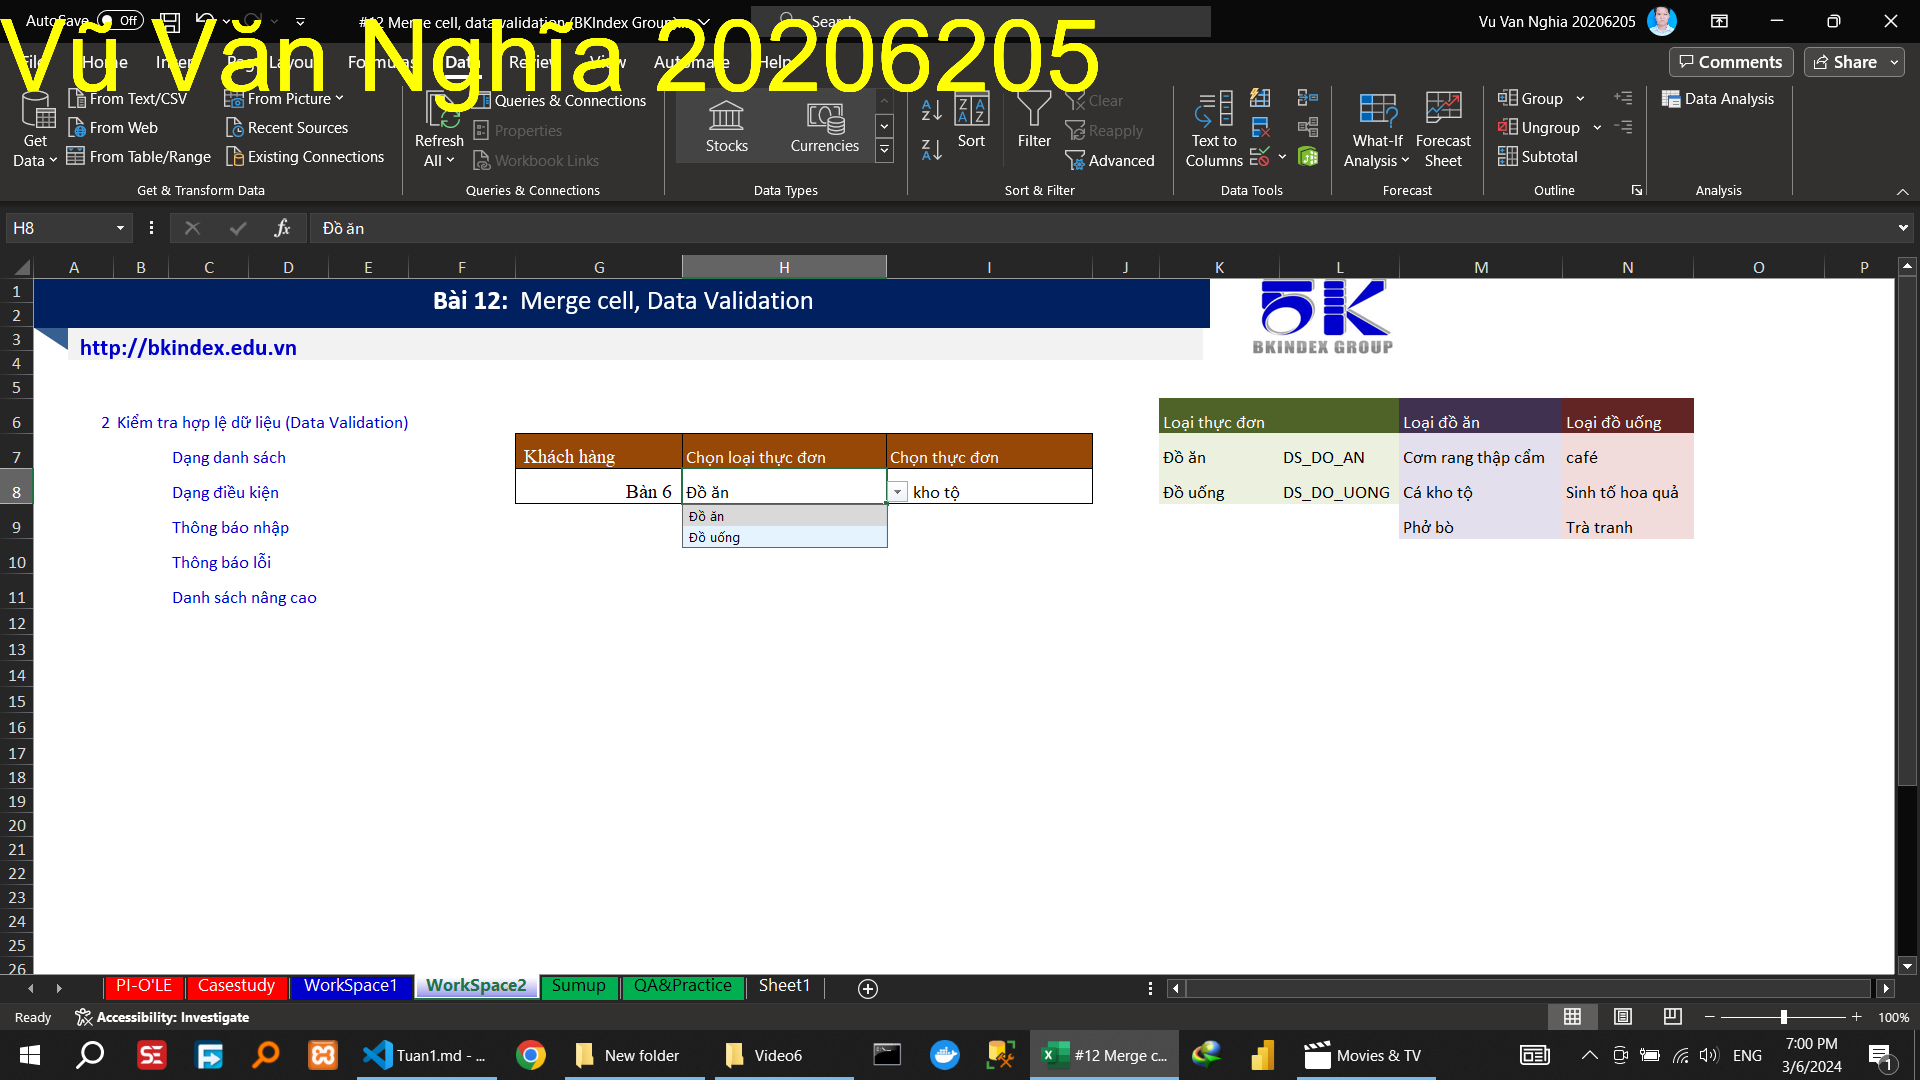
\includegraphics[scale = 0.15]{Video6/HuongDan/0.png}
\caption{Hướng dẫn kiểm tra hợp lệ dữ liệu dạng danh sách chọn đồ ăn, đồ uống}
\end{figure}

\begin{figure}[H]
\centering
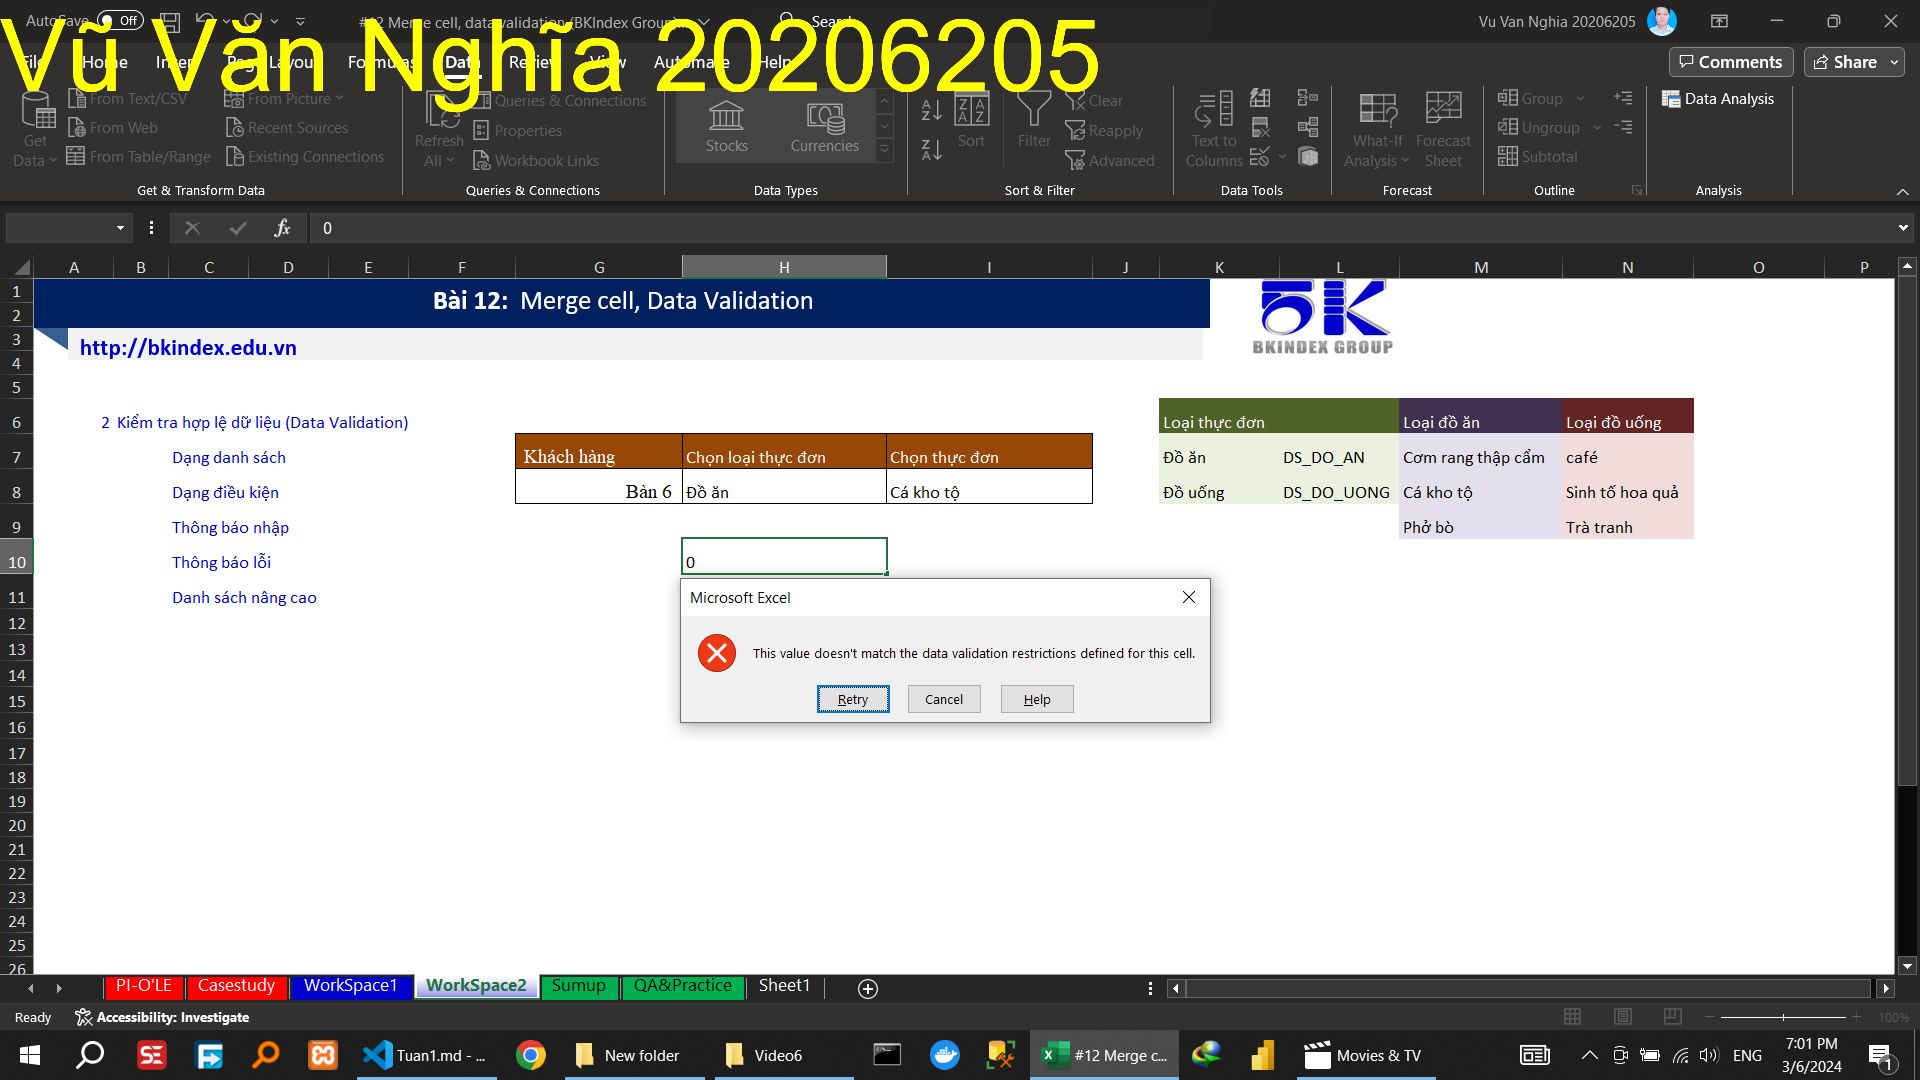
\includegraphics[scale = 0.15]{Video6/HuongDan/1.png}
\caption{Hướng dẫn kiểm tra hợp lệ dữ liệu dạng tùy chỉnh điều kiện lớn hơn 0}
\end{figure}

\begin{figure}[H]
\centering
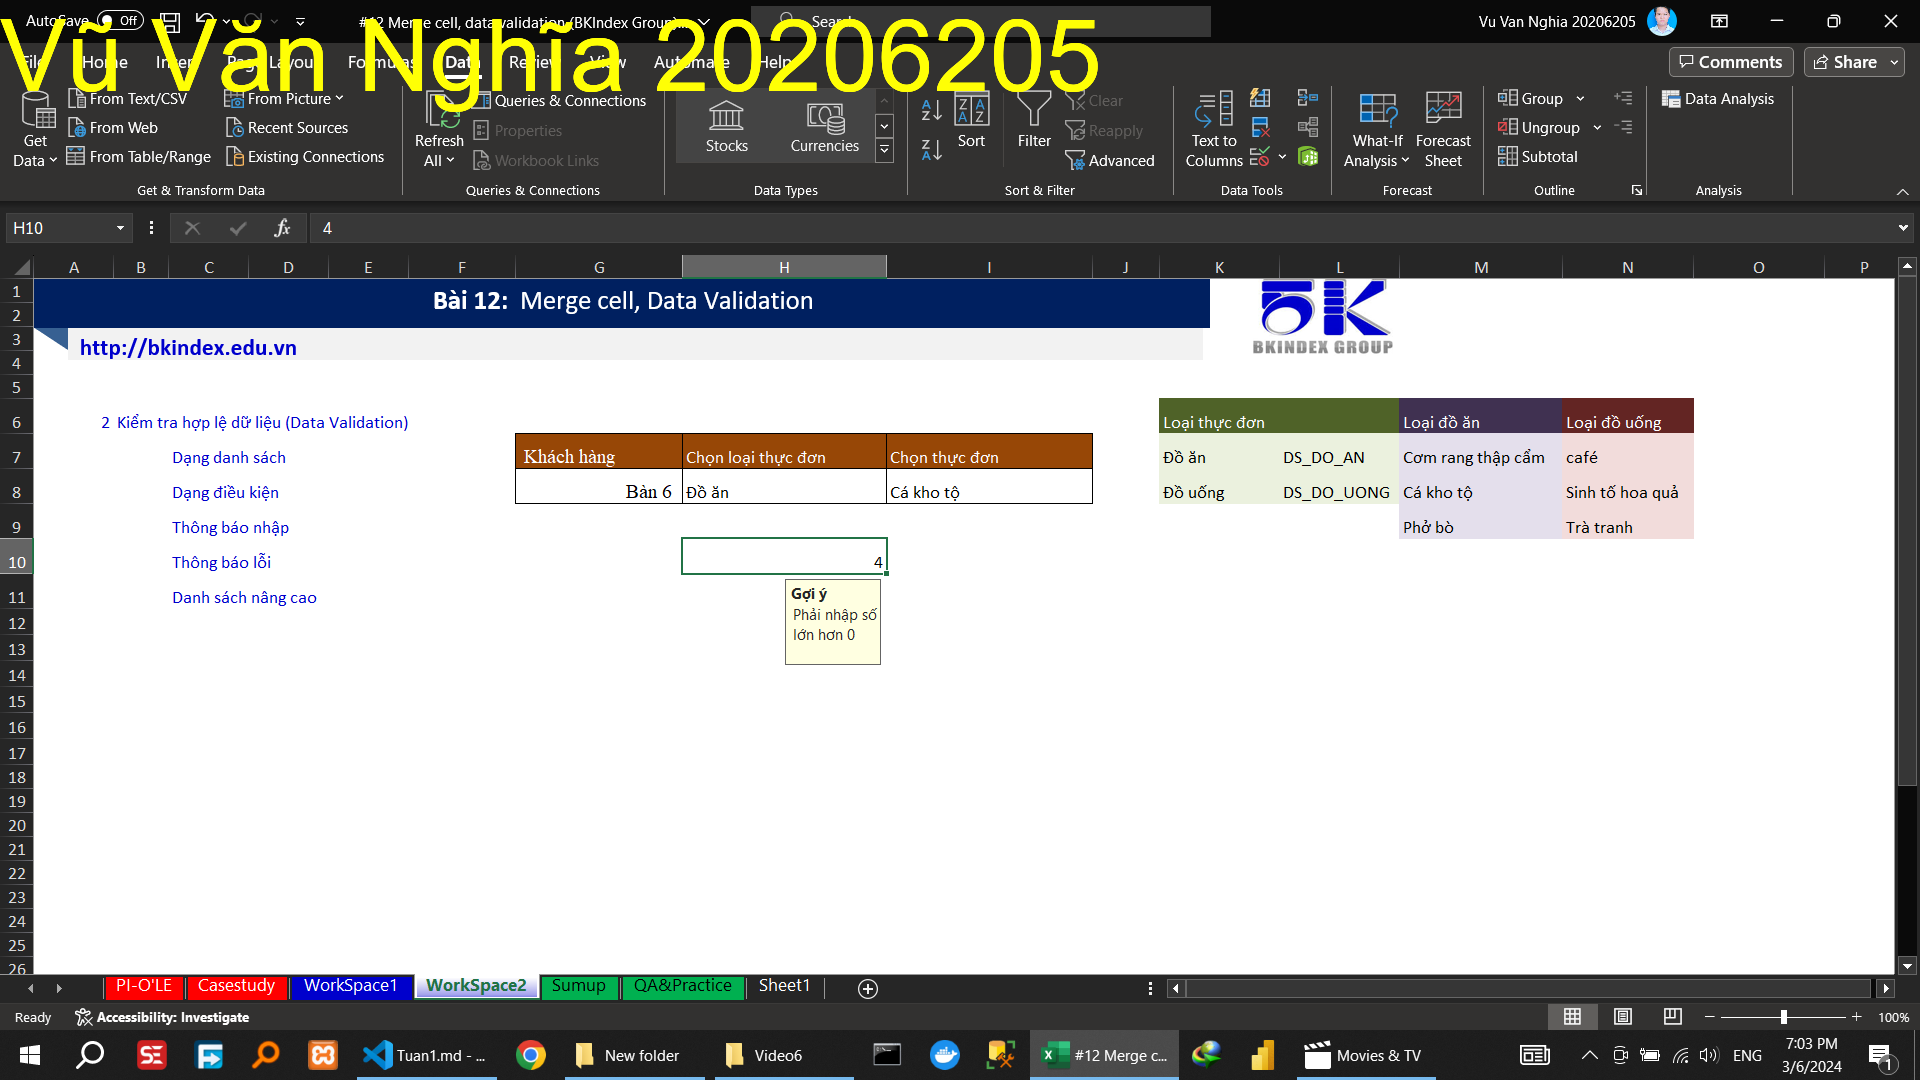
\includegraphics[scale = 0.15]{Video6/HuongDan/2.png}
\caption{Hướng dẫn hiện thông báo nhập phải nhập số lớn hơn 0}
\end{figure}

\begin{figure}[H]
\centering
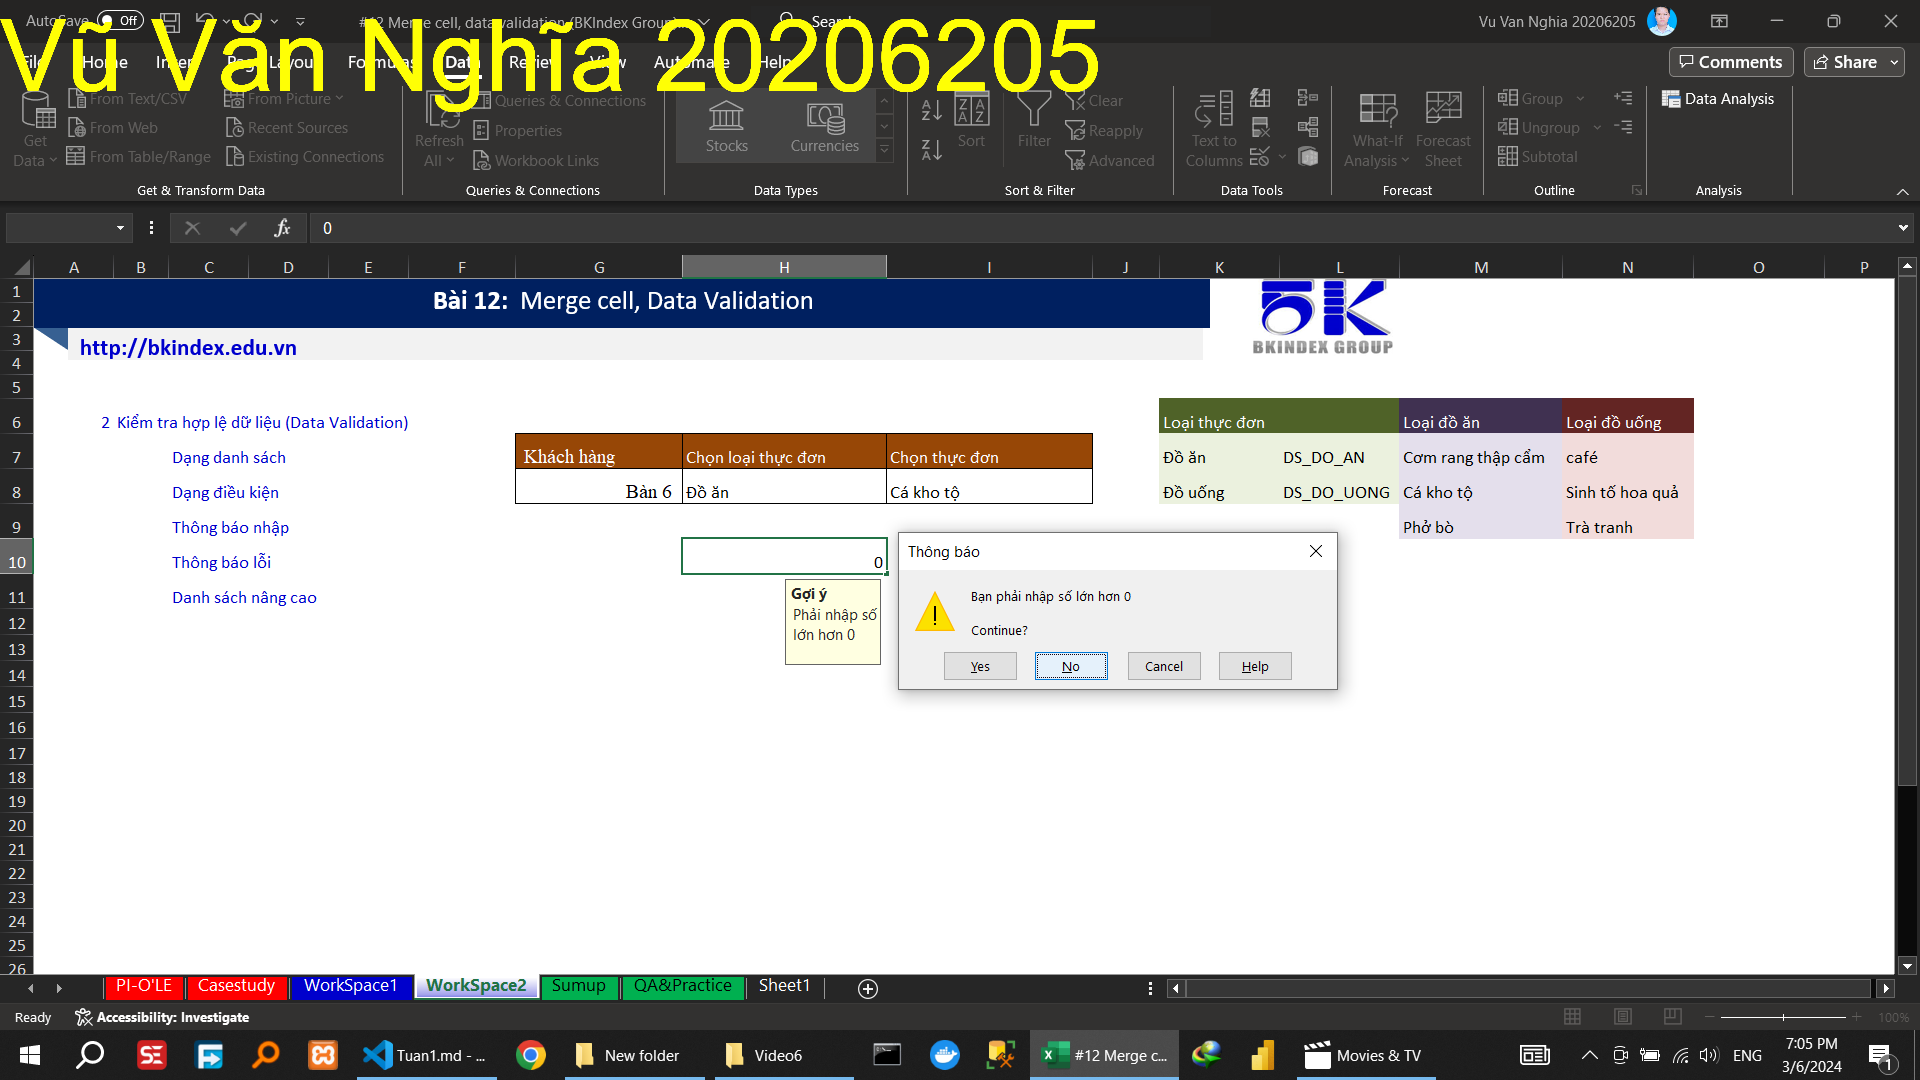
\includegraphics[scale = 0.15]{Video6/HuongDan/3.png}
\caption{Hướng dẫn hiện thông báo lỗi phải nhập số lớn hơn 0}
\end{figure}

\begin{figure}[H]
\centering
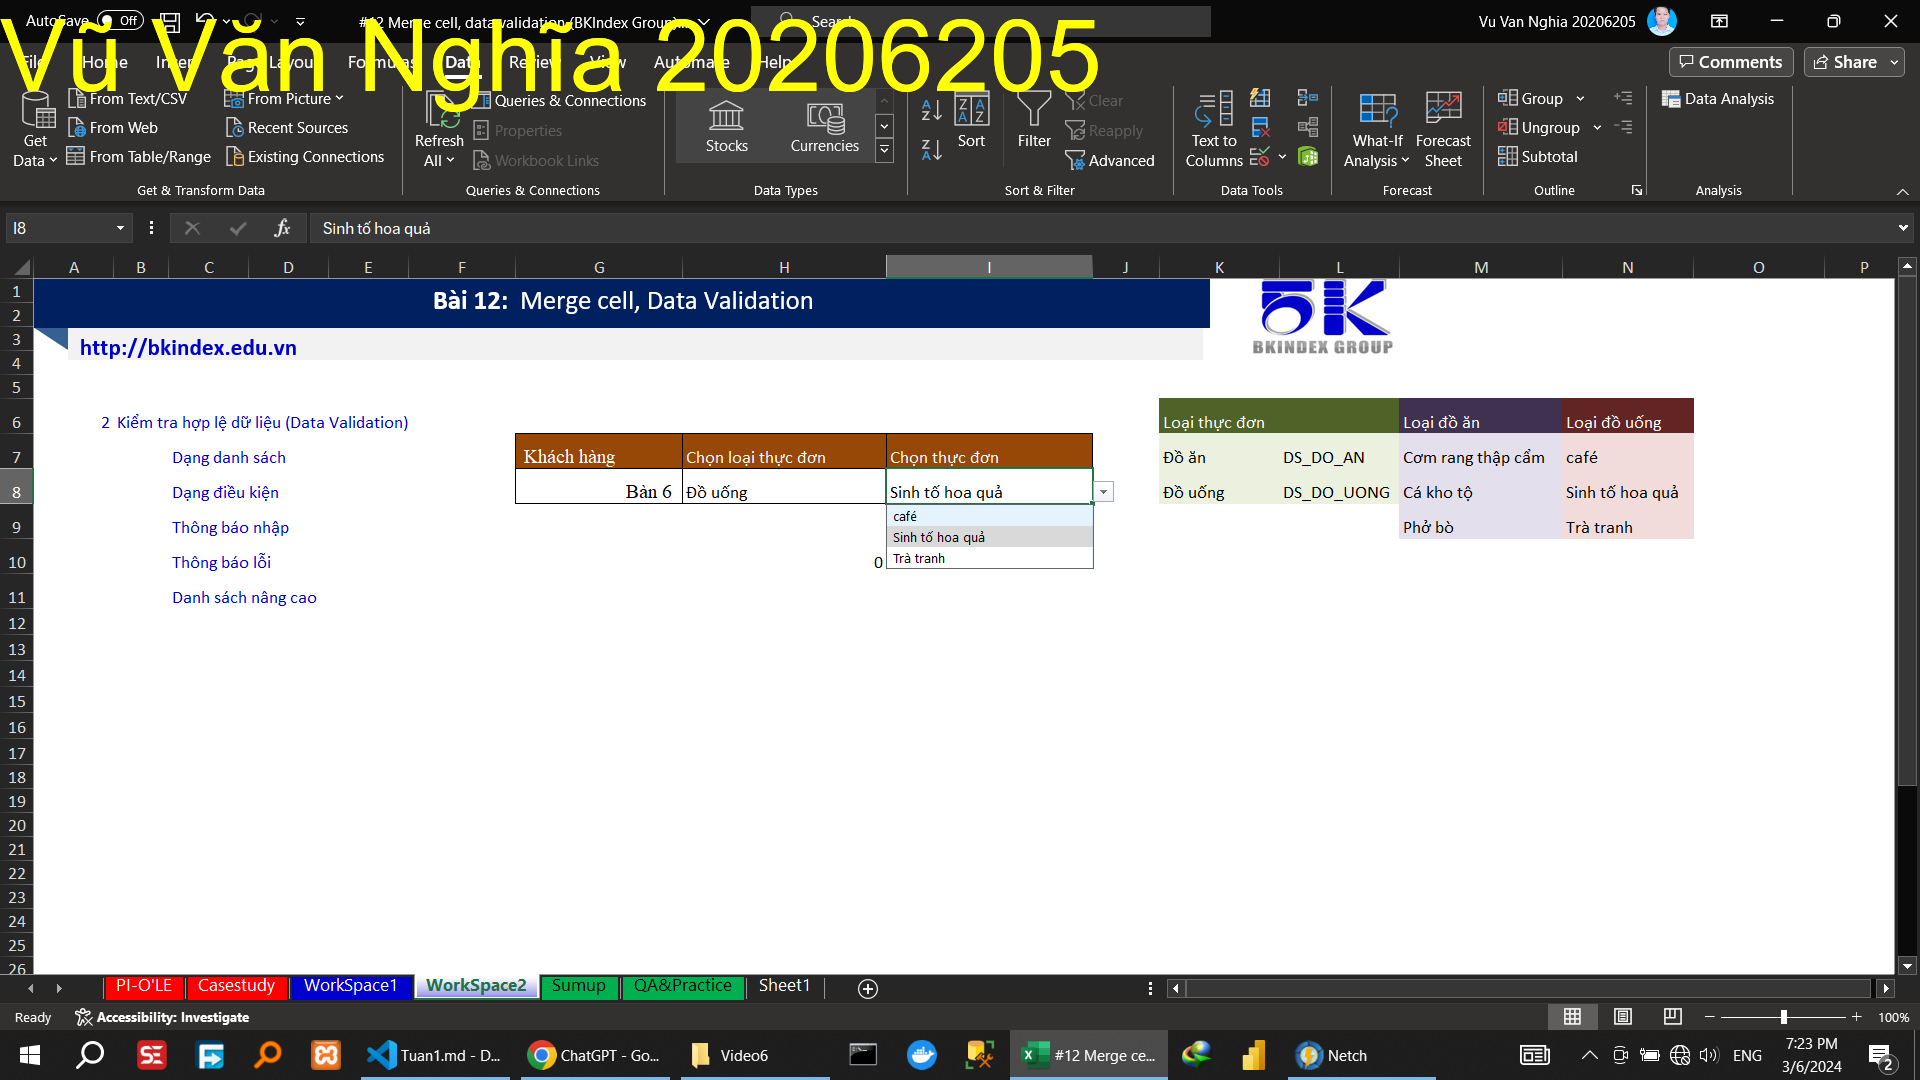
\includegraphics[scale = 0.15]{Video6/HuongDan/4.png}
\caption{Hướng dẫn sử dụng hàm indirect làm danh sách nâng cao đồ ăn, đồ uống}
\end{figure}
% %%%%%%%%%%%%%%%%%%%%%%%%%%%%%%%%%%%%%%%%%%%%%%%%%%%%%
\subsection{Video 7}
%%%%%%%%%%%%%%%%%%%%%%%%%%%%%%%%%%%%%%%%%%%%%%%%%%%%%
\begin{figure}[H]
\centering
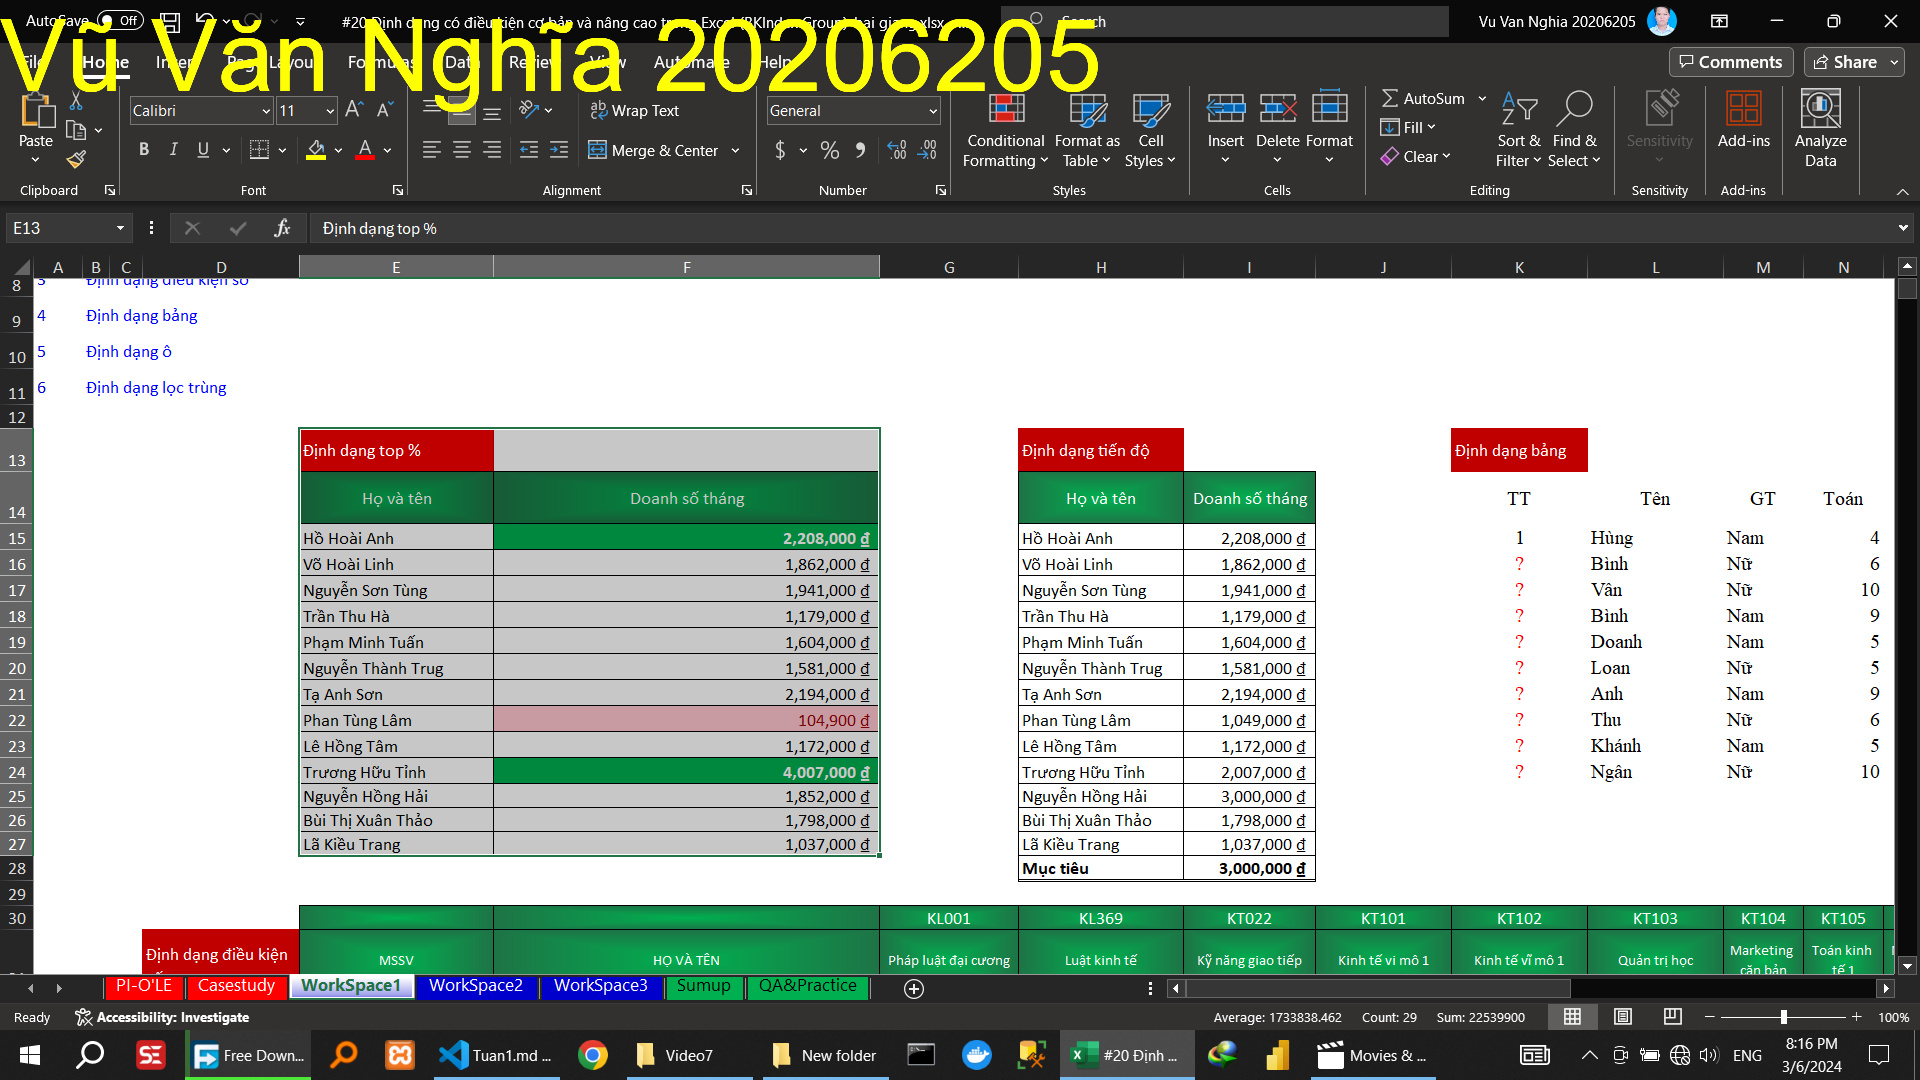
\includegraphics[scale = 0.15]{Video7/HuongDan/0.png}
\caption{Hướng dẫn định dạng top phần trăm}
\end{figure}

\begin{figure}[H]
\centering
\includegraphics[scale = 0.15]{Video7/HuongDan/1.png}
\caption{Hướng dẫn định dạng tiến độ}
\end{figure}

\begin{figure}[H]
\centering
\includegraphics[scale = 0.15]{Video7/HuongDan/2.png}
\caption{Hướng dẫn định dạng điều kiện số}
\end{figure}

\begin{figure}[H]
\centering
\includegraphics[scale = 0.15]{Video7/HuongDan/3.png}
\caption{Hướng dẫn định dạng bảng}
\end{figure}

\begin{figure}[H]
\centering
\includegraphics[scale = 0.15]{Video7/HuongDan/4.png}
\caption{Hướng dẫn định dạng ô}
\end{figure}

\begin{figure}[H]
\centering
\includegraphics[scale = 0.15]{Video7/HuongDan/5.png}
\caption{Hướng dẫn định dạng lọc trùng}
\end{figure}

\begin{figure}[H]
\centering
\includegraphics[scale = 0.15]{Video7/HuongDan/6.png}
\caption{Hướng dẫn xóa định dạng có điều kiện}
\end{figure}

\begin{figure}[H]
\centering
\includegraphics[scale = 0.15]{Video7/HuongDan/7.png}
\caption{Hướng dẫn quản lý các định dạng}
\end{figure}
%%%%%%%%%%%%%%%%%%%%%%%%%%%%%%%%%%%%%%%%%%%%%%%%%%%%%
\subsection{Video 8}
%%%%%%%%%%%%%%%%%%%%%%%%%%%%%%%%%%%%%%%%%%%%%%%%%%%%%
\begin{figure}[H]
\centering
\includegraphics[scale = 0.15]{Video8/HuongDan/0.png}
\caption{Hướng dẫn tự động định dạng dòng chẵn lẻ}
\end{figure}

\begin{figure}[H]
\centering
\includegraphics[scale = 0.15]{Video8/HuongDan/1.png}
\caption{Hướng dẫn định dạng dòng dựa vào 1 ô (trùng số CMND)}
\end{figure}

\begin{figure}[H]
\centering
\includegraphics[scale = 0.15]{Video8/HuongDan/2.png}
\caption{Hướng dẫn định dạng dòng theo ngày tham số (Năm sinh)}
\end{figure}

\begin{figure}[H]
\centering
\includegraphics[scale = 0.15]{Video8/HuongDan/3.png}
\caption{Hướng dẫn định dạng ô dựa vào 1 ô khác}
\end{figure}

\begin{figure}[H]
\centering
\includegraphics[scale = 0.15]{Video8/HuongDan/4.png}
\caption{Hướng dẫn định dạng ngày nghỉ}
\end{figure}
% %%%%%%%%%%%%%%%%%%%%%%%%%%%%%%%%%%%%%%%%%%%%%%%%%%%%%
% =MOD(ROW(C13), 2)=1
\begin{figure}[H]
\centering
\includegraphics[scale = 0.15]{Video8/ThucHanh/0.png}
\caption{Thực hành định dạng màu theo dòng }
\end{figure}

\begin{figure}[H]
\centering
\includegraphics[scale = 0.15]{Video8/ThucHanh/1.png}
\caption{Thực hành định dạng màu số HĐ theo quy định màu của mã phòng}
\end{figure}

% =$L11-TODAY()<30
\begin{figure}[H]
\centering
\includegraphics[scale = 0.15]{Video8/ThucHanh/2.png}
\caption{Thực hành định dạng màu: Nhân viên sắp hết hạn hợp đồng lao động (trong 30 ngày tới sẽ hết hạn)}
\end{figure}

% =AND($M11>=8000000, $M11<=10000000)
\begin{figure}[H]
\centering
\includegraphics[scale = 0.15]{Video8/ThucHanh/3.png}
\caption{Thực hành định dạng màu: Nhân viên có mức lương từ 8 đến 10 triệu}
\end{figure}

% =$F11=""
\begin{figure}[H]
\centering
\includegraphics[scale = 0.15]{Video8/ThucHanh/4.png}
\caption{Thực hành định dạng màu: Nhân viên chưa có thông tin CMND}
\end{figure}

% =DATEDIF($G11, TODAY(), "y") > 15
\begin{figure}[H]
\centering
\includegraphics[scale = 0.15]{Video8/ThucHanh/5.png}
\caption{Thực hành định dạng màu: Nhân viên đã hết hạn CMTND (cấp quá 15 năm)}
\end{figure}

% =AND($C11="Kho", $H11="Hà Nội")
\begin{figure}[H]
\centering
\includegraphics[scale = 0.15]{Video8/ThucHanh/6.png}
\caption{Thực hành định dạng màu: Nhân viên bộ phận kho có hộ khẩu tại HN để lên lịch trực tết}
\end{figure}
%%%%%%%%%%%%%%%%%%%%%%%%%%%%%%%%%%%%%%%%%%%%%%%%%%%%%%%
\end{document}
%%%%%%%%%%%%%%%%%%%%%%%%%%%%%%%%%%%%%%%%%%%%%%%%%%%%%%%